\documentclass[11pt,a4paper]{article}
\usepackage[UTF8,fontset=fandol]{ctex}
\usepackage{amsmath,amssymb,amsthm,mathtools}
\usepackage{lmodern}
\usepackage{graphicx}
\graphicspath{{./}{reports/figures_v2/}{reports_v3/figures/}}
\usepackage{tikz}
\usetikzlibrary{shapes.geometric, arrows.meta, positioning, calc, backgrounds, fit}
\usepackage{geometry}
\geometry{left=1.85cm,right=1.85cm,top=2.0cm,bottom=2.0cm}
\setlength{\textfloatsep}{6pt plus 2pt minus 2pt}
\setlength{\floatsep}{4pt plus 2pt minus 2pt}
\setlength{\intextsep}{4pt plus 2pt minus 2pt}
\setlength{\parskip}{0pt}
\setlength{\abovedisplayskip}{4pt plus 1pt minus 1pt}
\setlength{\belowdisplayskip}{4pt plus 1pt minus 1pt}
\setlength{\abovedisplayshortskip}{1pt plus 1pt}
\setlength{\belowdisplayshortskip}{1pt plus 1pt}
\renewcommand{\topfraction}{0.92}
\renewcommand{\bottomfraction}{0.85}
\renewcommand{\textfraction}{0.08}
\renewcommand{\floatpagefraction}{0.85}
\emergencystretch=3em
\usepackage{enumitem}
\setlist{itemsep=1.5pt,topsep=2.5pt,partopsep=0pt,parsep=0pt}
\usepackage{xurl}
\usepackage{hyperref}
\hypersetup{
    colorlinks=true,
    linkcolor=black,
    citecolor=blue!80!black,
    urlcolor=blue!80!black
}
\usepackage{booktabs}
\usepackage{rotating}
\usepackage{array}
\usepackage{multirow}
\usepackage[numbers,sort&compress]{natbib}
\usepackage{multicol}
\usepackage{titlesec}
\usepackage{caption}
\usepackage{fancyhdr}
\captionsetup{labelsep=quad,labelfont=bf,textfont=small,justification=justified}

% Custom section formatting according to Chinese journal style using titlesec
\titleformat{\section}{\raggedright\heiti\zihao{4}\bfseries}{\thesection}{0.5em}{}
\titleformat{\subsection}{\raggedright\heiti\zihao{4}\bfseries}{\thesubsection}{0.5em}{}
\titleformat{\subsubsection}{\raggedright\heiti\zihao{5}\bfseries}{\thesubsubsection}{0.5em}{}
\titlespacing*{\section}{0pt}{1.0ex plus .2ex minus .1ex}{0.6ex plus .1ex}
\titlespacing*{\subsection}{0pt}{0.8ex plus .2ex minus .1ex}{0.5ex plus .1ex}
\titlespacing*{\subsubsection}{0pt}{0.6ex plus .1ex minus .1ex}{0.4ex plus .1ex}

% Theorem environments
\theoremstyle{plain}
\newtheorem{theorem}{定理}
\newtheorem{proposition}{命题}
\newtheorem{lemma}{引理}
\newtheorem{corollary}{推论}
\theoremstyle{definition}
\newtheorem{definition}{定义}
\newtheorem*{remark}{注记}

% Remove LaTeX default proof square box (keep only Chinese '证毕。')
\renewcommand{\qedsymbol}{}

% Visual styling colors for TikZ and graphics
\definecolor{navyMain}{RGB}{18, 42, 77}
\definecolor{slateGray}{RGB}{70, 80, 95}
\definecolor{boxBg}{RGB}{250, 252, 255}
\definecolor{subBg}{RGB}{245, 248, 252}
\definecolor{borderCol}{RGB}{75, 95, 125}

\pagestyle{fancy}
\fancyhf{}
\fancyhead[C]{\footnotesize 传染病预测视界的机制基准与实证校准差距}
\fancyfoot[C]{\footnotesize\thepage}
\renewcommand{\headrulewidth}{0.4pt}
\begin{document}
\thispagestyle{plain}
% Section numbering starts from 1

% Title (without author placeholders)
\begin{center}
    \vspace*{-0.6em}
    {\zihao{2}\heiti\bfseries 传染病预测视界的机制基准与实证校准差距} \\[0.4em]
\end{center}

% Abstract & Keywords Box
{\small
\noindent{\heiti\bfseries 摘要：}重大呼吸道传染病的前瞻预测在传播阈值临界点及多周外推中常出现系统性的技能衰减与校准恶化。本文旨在厘清理论机制方差、现实预测误差与系统校准差距三者的内在关联。方法上，本文在信息集可测规则类中证明条件平方风险恒等式，确立条件均值预测器所达到的锐条件方差地板；建立个体分支与宏观更新的尺度隔离框架，推导固定离散度宏观负二项更新模型的精确有限步方差闭式与其数值稳定边界极限，并解析刻画对数正态参数推断误差的非线性指数外推放大项与代入式预测器的超额风险。全文构建包含理论仿真、个体传播链、州级住院面板与预测枢纽的四层证据架构，外部审计对接美国 CDC FluSight 连续三个锁定历史赛季（覆盖 2021--2026 年七个呼吸道流行阶段）。

结果表明，数值模拟在全网格上核验了宏观方差闭式（相对偏差集中于 $1\%\sim 3\%$）；微观传播链拟合中负二项模型获得远低于 Poisson 的 AIC（$\Delta\text{AIC}$ 达 93.9--244.0，相对拟合表现明显更优）；在覆盖美国最多 51 个州级辖区的住院面板上（各阶段满足最低发病门槛的辖区数为 26--51，详见第 5.1 节），5 周基准滑动窗口下插件式 NB2 机制视界的州级中位数为 2.2--7.1 周（预设 5--10 周窗口敏感性变动为 $-48.7\%$ 至 $+44.6\%$，多窗口极值包络覆盖 1.52--8.07 周；放宽准入门槛至 $\ge 10$ 例后该跨阶段区间下移至 1.73--6.81 周，表明低计数阶段的中位视界被系统性高估）；描述性误差记账显示 21 个配置中模型—观测代数差额跨州中位占比中位数为 $55.0\%$（$h=1$ 为 $45.4\%$，21 个配置中有 20 个的跨州中位差额为正），表明显式机制分量在多数配置中未能完全覆盖实测误差。以终报数据驱动的受控诊断性基准开展 FluSight 外部审计显示，仅依赖机制方差的插件式预测器存在显著经验欠覆盖（标称 95\% 预测区间实测覆盖率仅 0.405--0.554，平均区间宽度显著收窄 12.6\%--44.6\%）；事后识别的全局峰值相对位置分层进一步证实，各模型在峰前期普遍面临经验覆盖率骤降（2025--26 赛季在 $n=43$ 的小样本下 Hub 集成 95\% 覆盖率降至 0.419，机制预测器降至 0.140；全三赛季峰前期覆盖率为 0.140--0.852，峰后期恢复至 0.925--0.964）。

结论表明，机制视界本质上是依赖模型、信息集与指定规则的条件机制基准，在本文 NB2 工作模型与同定义汇总比较口径下，形成现实业务预警时效的宽松经验参考外包络。本框架为定量诊断传染病预测校准差距提供了系统性工具，提示未来业务系统应重点评估实时数据回填建模与面向峰前期的动态不确定性膨胀机制。

\vspace{0.2em}
\noindent{\heiti\bfseries 关键词：}传染病预测；可预测视界；更新模型；分支过程；机制基准；校准差距；加权区间评分
}

\vspace{0.6em}

\section{引言}\label{sec:intro}

\subsection{研究背景与现实困境}

重大呼吸道传染病（如新型冠状病毒感染、季节性流感与呼吸道合胞病毒 RSV）的周期性暴发对全球公共卫生与医疗体系构成长期挑战。在疫情早期的动态演化中，及时可靠的前瞻预测是优化重症资源配置、预置抗病毒药物与启动非药物干预（NPI）的关键支撑。然而，传染病前瞻预测在实务中频繁遭遇系统性失效瓶颈：当疫情处于平稳指数增长或下降阶段时，现有统计与动力学模型通常能保持较高准确度；但一旦逼近流行阈值（即基本再生数 $R \approx 1$ 的临界点）或开展多周前瞻外推，预测系统的性能便发生系统性劣化：预测区间急剧发散、预测轨迹频繁出现预测性能骤降与严重失准\citep{reich2019collaborative}。Scarpino 与 Petri\citep{scarpino2019predictability} 基于信息论与排列熵（Permutation Entropy）刻画了疫情在流行阈值附近的无模型（Model-Free）内在可预测性突变；然而，无模型排列熵界主要反映时间序列本身的统计可压缩性，未显式给出特定生成机制下有限步前瞻方差的累积律与参数推断误差的传播闭式。

为应对传染病前瞻预测的重大现实需求，计算流行病学形成了四类代表性建模范式：(1) 基于房室微分方程的机理动力学模型（如经典 SIR/SEIR 及其随机拓展）；(2) 基于统计推断的时序更新模型（如滑动自回归、更新方程与再生数实时推断）；(3) 数据驱动的机器学习流派（如循环神经网络与时空图网络）；(4) 多模型概率预报集成。

然而，跨越多年与多病种的大规模协同预测评估揭示了长期制约前瞻预测实践的结构性瓶颈。无论是美国 CDC FluSight 流感预测\citep{mcgowan2019collaborative, flusight2024evaluation}、RAPIDD 埃博拉评估\citep{viboud2018rapidd}、登革热预测挑战\citep{johansson2019open}，还是欧美 COVID-19 预测枢纽\citep{cramer2022evaluation, sherratt2023europeanhubs}，评估结果均表明：在多周前瞻外推（3--4 周及以上）或波次起伏临界期，绝大多数复杂流行病学模型的实测预测技巧均迅速衰减，甚至难以稳定优于简单的持续性基线或局部线性外推模型\citep{suez2026baseline, lopez2024challenges}。此外，早期监测数据普遍存在的报告延迟与漏报回填，使得远期外推面临严重的实用不可识别性（Practical Unidentifiability）\citep{melikechi2022limits, king2015avoidable}。

\subsection{本文主要贡献与结构安排}

针对上述理论空白与现实困境，本文的主要贡献体现在以下四个方面：
\begin{enumerate}
\item \textbf{锐条件方差地板与宏观更新有限步精确方差闭式}：在信息集 $\mathcal{F}_t$ 的二阶可积预测规则类上证明平方损失下的条件风险恒等式（定理~\ref{thm:sharp_floor}），确立条件均值预测器达到的锐条件方差地板。建立个体分支与宏观更新的尺度隔离框架，推导固定离散度 $k_{\text{agg}}$ 宏观负二项更新模型的精确有限步方差闭式（定理~\ref{thm:macro_exact}）及其数值稳定边界极限与严格单调求根方程。
\item \textbf{参数后验对数正态混合与信息论识别极限}：解析刻画对数正态参数推断误差的指数型前向放大项 $P_{\text{exact}}(h)$（引理~\ref{lem:param_amplification}）与代入式预测器的超额风险；证明对数正态后验下的全方差分解有限和形式（命题~\ref{prop:posterior_mixture}）；推导负二项分支过程的 Fisher 信息量与 Cramér--Rao 理想样本量基准（定理~\ref{thm:fisher}），明确限定其为理想模型内的辨识下限（$C = O(\varepsilon^{-2})$）。
\item \textbf{四层证据架构与模型—观测差额诊断}：构建包含理论模拟、个体传播链、州级住院面板与国家级预测枢纽的四层证据架构。在覆盖美国最多 51 个州级辖区的住院面板上（各阶段满足数据充分性门槛的辖区数为 26--51），测得 5 周基准滑动窗口下插件式 NB2 机制视界中位数为 2.2--7.1 周；通过描述性误差记账发现 21 个配置中模型—观测代数差额跨州中位占比中位数为 $55.0\%$（$h=1$ 为 $45.4\%$，21 个配置中有 20 个为正），表明特定更新机制分量不足以包络现实总误差，据此将机制视界定位为现实预警时效的宽松经验参考外包络。
\item \textbf{三赛季版本化外部审计与阶段校准特征}：全面接入 CDC FluSight 连续三个锁定历史赛季（v1.0.0--v1.2.0 共 204 个固化输入文件，逐文件 SHA-256 校验固化）。以终报数据驱动的受控诊断性基准实测揭示机制基准存在显著的经验欠覆盖与校准偏离（标称 95\% 覆盖率仅 0.405--0.554，区间宽度偏窄 12.6\%--44.6\%）；全局峰值相对位置事后分层进一步发现各模型在峰前期普遍面临经验覆盖率骤降（Hub 集成降至 0.419--0.852，机制预测器仅 0.140--0.385；峰后期集成恢复至 0.925--0.964），为业务预测系统的动态方差膨胀与敏捷公卫应急提供了实证线索。
\end{enumerate}

\subsection{证据架构与方法学边界}\label{sec:claim_hierarchy}

为确保学术推论的严谨性与概念边界的清晰性，表~\ref{tab:claim_hierarchy} 系统确立了全文数理推导、仿真实验与多层实证成果的证据层级，明确划定每项成果严格支持的科学推论及其方法学适用边界与解释限制。全文所有术语（如“机制基准”、“条件方差地板”、“模型—观测代数差额”）均在此层级规范下严格使用。

本文结构安排如下：第 1 节阐述背景与贡献；第 2 节回顾理论文献；第 3 节建立传播动力学可预测视界理论；第 4 节给出高通量数值验证；第 5 节报告微观传播链与州级住院面板实证；第 6 节开展 CDC FluSight 外部审计与校准差距分析；第 7 节讨论决策转化与局限；第 8 节总结全文。核心定理证明要点与全景索引见附录，详尽推导演算参见补充材料《Supplementary Mathematical Derivations》。

\begin{table}[t]
\centering
\fontsize{7.0pt}{8.6pt}\selectfont
\setlength{\tabcolsep}{2.0pt}
\caption{本文证据架构与方法学适用边界界定表}
\label{tab:claim_hierarchy}
\begin{tabular}{@{}>{\raggedright\arraybackslash}p{2.6cm}>{\raggedright\arraybackslash}p{4.2cm}>{\raggedright\arraybackslash}p{4.2cm}>{\raggedright\arraybackslash}p{4.5cm}@{}}
\toprule
证据层级 & 关键数理／实证结果 & 严格支持的科学推论 & \textbf{适用边界与解释限制} \\
\midrule
\textbf{理论地板层}：条件风险恒等式（定理~\ref{thm:sharp_floor}） & 任意 $\mathcal{F}_t$-可测决策规则在平方损失下的条件风险正交分解：$\mathcal{R}_h(\delta_h\mid\mathcal{F}_t) = V_h + (m_h - \delta_h)^2$ & 条件均值唯一达到给定概率模型与信息集下的平方风险地板；进一步定义的预测视界还依赖预测规则、损失函数、归一化方式和容忍度阈值 & 条件方差 $V_h$ 刻画给定模型与信息集内的不可约方差极限，不直接等同于现实异质传播系统的通用物理下界；现实预测器亦不保证自动逼近该界 \\
\addlinespace[1.5pt]
\textbf{微观分支层}：饱和极限与模型内有效性（引理~\ref{lem:cv_floor}、定理~\ref{thm:fisher}） & 负二项 Galton--Watson 过程内在相对方差饱和于 $\text{CV}^2_\infty$；三组权威传播链负二项 AIC 明显低于 Poisson（$\Delta\text{AIC} = 93.9\text{--}244.0$）且在所用优度检验下未被拒绝 & 确立了个体级超级传播过度离散在微观数据上的相对拟合优势；证实该特定负二项似然下极大似然估计具备模型内自洽性 & 微观分支方差闭式反映个体接触网络的随机性，不直接等同于宏观周度聚合序列；负二项分布属于相对优选模型，并非自然界唯一排他机制 \\
\addlinespace[1.5pt]
\textbf{宏观更新层}：固定参数 NB2 模型内方差（定理~\ref{thm:macro_exact}） & 周度宏观负二项聚合更新工作模型的精确有限步方差闭式，含 $[(1+1/k_{\text{agg}})^h - 1]$ 几何发散主项 & 在给定 NB2 宏观生成过程与固定 $k_{\text{agg}}$ 条件下，解析刻画了宏观过程离散度随步长的递推演化与边界极限 & 几何累积项特定于固定 $k_{\text{agg}}$ 的 NB2 二次过度离散结构；Poisson 或 NB1 设定下超临界相对方差呈有界饱和，状态空间模型亦受潜状态平滑约束 \\
\addlinespace[1.5pt]
\textbf{参数外推层}：对数正态放大与信息界（引理~\ref{lem:param_amplification}、定理~\ref{thm:fisher}） & 对数正态参数估计误差经指数外推导致的超额相对均方误差闭式 $P_{\text{exact}}(h)$（领先阶为 $P_{\text{quad}}$）；负二项分支过程单代极大似然的 Fisher 信息量与 CRB 下界 & 量化代入式点估计预测器在参数不确定性下的超额风险；确立理想无偏估计下的参数辨识样本量阶数 $O(\varepsilon^{-2})$ & 参数放大项 $P_{\text{exact}}$ 针对点估计代入式外推，不替代完整贝叶斯后验积分；理想 CRB 样本量未计入现实流调中的严重漏报与数据回填噪声 \\
\addlinespace[1.5pt]
\textbf{州级实证层}：机制视界与误差记账（第 5 节） & 美国最多 51 个州级辖区住院面板（逐阶段 26--51）测得插件式 NB2 机制视界中位数为 2.2--7.1 周；两项显式模型分量与一项模型—观测代数差额中 21 个配置跨州中位代数差额占比的中位数为 $55.0\%$（$h=1$ 为 $45.4\%$） & 在多数阶段—步长配置中，当前工作模型下的显式机制分量不能充分覆盖实测误差；但该关系具有明显阶段异质性，部分短步长或低残差配置中机制分量可接近实测误差；机制视界构成现实业务预警时效的宽松经验参考外包络 & 代数差额反映描述性误差构成，非因果正交方差分解；机制视界受推断窗口选择影响（5--10 周敏感性变动为 $-48.7\%\sim +44.6\%$，多窗口极值包络 1.52--8.07 周） \\
\addlinespace[1.5pt]
\textbf{外部审计层}：CDC FluSight 三赛季审计（第 6.1--6.4 节） & 连续三赛季严格四方共同单元审计证实 Hub 集成持续优于基线；启发式插件式机制预测器严重欠覆盖（0.405--0.554）；多个模型—赛季组合在事后划分的峰前期经验覆盖率较低 & 量化启发式插件式机制预测器与历史业务预测系统之间的经验评分及校准差距，并据此诊断仅依赖模型内机制方差构造预测分布的局限；为多个模型—赛季组合在峰前期出现覆盖率明显下降提供描述性证据，为动态方差膨胀提供实证线索 & 峰前期覆盖率下降混杂了结构变点、行为适应与数据回填等多重现实因素；机制预测器享有终报数据质量优势，在方法学上定位于受控诊断基准 \\
\addlinespace[1.5pt]
\textbf{跨病原对照层}：COVIDhub 12 原点历史审计（第 6.5 节） & COVIDhub-ensemble 在 Delta 与 Omicron 暴发期的 12 个预测原点中有 11 个在 1--2 周内达到或穿透持续性基线平价线 & 为流感与 COVID-19 快速扩散期短步长预测技能衰减提供了跨病原的描述性支持，但尚不足以证明所有重大呼吸道传染病均存在同一机制瓶颈 & 实证基于 COVID-19 与流感回溯审计，外推至 RSV 等尚缺官方协同预报枢纽的病种需审慎验证；多模型集成无法无条件突破短时效瓶颈 \\
\bottomrule
\end{tabular}%
\end{table}

\section{研究回顾}\label{sec:review}

\subsection{相关研究回顾与理论脉络}

面对前瞻预测精度的急剧衰退，现有文献主要沿四条脉络探索其内在机制与可预测性边界：

第一，\textbf{随机分支过程与概率更新推断}。Galton--Watson 负二项分支过程\citep{athreya1972branching}与更新方程为刻画个体超扩散提供了经典的统计似然基础\citep{lloyd-smith2005superspreading}。在群体推断层面，Cori 等\citep{cori2013framework}与 Gostic 等\citep{gostic2020practical}确立了时变再生数 $R_t$ 的贝叶斯滤波推断规范；Parag 等\citep{parag2020information, parag2022fundamental, parag2022quantifying}进一步从信息论视角揭示了发病曲线反演再生数所固有的代间隔检测延迟与信息瓶颈。关于更新过程的方差演化与过度离散建模，自回归与负二项监测框架可追溯至 Held 等\citep{held2017monitoring}及早期分支过程方差递推（如 Drake\citep{drake2006limits}）。然而，经典文献对多步前瞻条件方差多依赖递归数值卷积或蒙特卡洛仿真。本文在此脉络上推进，聚焦于离散周度尺度的固定离散度 NB2 宏观更新模型，通过对代间隔递推关系实施裂项求和，首次解析推导了任意有限提前期 $h$ 的精确方差闭式解（定理~\ref{thm:macro_exact}），并由此逆解出机制预测视界的解析求根方程。

第二，\textbf{生态预测视界与操作性时效架构}。在理论生态学领域，Petchey 等\citep{petchey2015ecological}将“生态预测视界”（Ecological Forecast Horizon）形式化定义为预测误差首次达到预设容忍度门槛的时间距离，并强调视界是依赖系统内在动力学、外生扰动、模型规则与损失函数的操作性构造。近期，Wesselkamp 等\citep{wesselkamp2025forecast}重新审视了生态预测极限，指出确定性非线性系统与随机生灭过程在可预测时间尺度上存在本质差异。针对流行病领域，Bozzuto 与 Ives\citep{bozzuto2023differences}在全美州县级尺度测算了 COVID-19 的模型无关时间序列可预测视界（约 8--9 周），发现宏观聚集与防控措施显著改变了可预测性空间分布。此外，Penn 等\citep{penn2023intrinsic}明确区分了模型内在随机性与统计认知不确定性，本文在此框架基础上推进了具体的方差闭式求解与视界解析反演。

第三，\textbf{统计物理临界慢化与拟平稳涨落}。在统计物理与非线性动力学中，系统在相变临界点附近普遍出现临界慢化（Critical Slowing Down）与涨落发散\citep{grassberger1983critical}。流行病学研究亦将这一现象作为暴发早期的预警信号（Early Warning Signals）\citep{oregan2013theory, southall2021early}。在有限宿主群体中，吸收态马尔可夫链的拟平稳分布（Quasi-Stationary Distribution, QSD）刻画了灭绝与暴发之间的亚稳态长尾涨落\citep{darroch1965quasi, nasell1999quasi, dolgoarshinnykh2006critical}。然而，此类微观扩散标度主要提供定性的动力学直觉，尚缺乏连接宏观周度发病序列的具体闭式映射。

第四，\textbf{信息论推断极限与两类可预测性概念}。在统计推断领域，必须严格区分两类可预测性概念：基于时间序列排列熵与相空间重构的内在可预测性（如 Song 等\citep{song2010limits}与 White 等\citep{white2026forecastability}），回答序列本身蕴含多少可压缩信息；以及基于统计推断与似然理论的估计精度下界（如 Cramér--Rao 下界）\citep{parag2022fundamental}。本文属于后者：我们在负二项随机生成模型下，以条件方差地板与 Fisher 信息量界定推断精度下限，进而通过误差传播推导宏观前瞻预测视界的机制基准。

\section{传播动力学可预测视界理论}

\subsection{观测尺度、信息集与锐条件平方风险地板}\label{sec:risk_floor}

考虑离散时间下的周度宏观发病与住院监测序列 $\{Z_t\}_{t \ge 0}$，其中 $Z_t \in \mathbb{N}$ 表示第 $t$ 周内全部辖区报告的新发病例数。设概率空间为 $(\Omega, \mathcal{A}, \mathbb{P})$，预测原点 $t$ 历史可得的全部信息构成 $\sigma$-代数流 $\mathcal{F}_t = \sigma(Z_0, Z_1, \dots, Z_t; \mathbf{X}_t)$，其中 $\mathbf{X}_t$ 包含原点前严格可得的外生协变量或历史数据修订记录。

预测目标为前瞻提前期（Horizon）$h \ge 1$ 步的真实状态变量 $Y_{t+h}$（在最终核准真值口径下 $Y_{t+h} = Z_{t+h}$）。定义允许的预测规则集合为 $\mathcal{F}_t$-可测且二阶可积的实随机变量类：
\begin{equation}
\mathcal{D}_t \equiv L^2(\Omega, \mathcal{F}_t, \mathbb{P}) = \left\{ \delta_h : \Omega \to \mathbb{R} \;\middle|\; \delta_h \text{ 为 } \mathcal{F}_t\text{-可测}, \; \mathbb{E}[\delta_h^2] < \infty \right\}.
\end{equation}
记目标变量在当前信息集 $\mathcal{F}_t$ 下的条件期望与条件方差分别为：
\begin{equation}
m_h \equiv \mathbb{E}[Y_{t+h} \mid \mathcal{F}_t], \qquad V_h \equiv \operatorname{Var}(Y_{t+h} \mid \mathcal{F}_t).
\end{equation}

在平方损失 $L(y, \delta) = (y - \delta)^2$ 下，定义预测规则 $\delta_h \in \mathcal{D}_t$ 的条件平方预测风险为 $\mathcal{R}_h(\delta_h \mid \mathcal{F}_t) \equiv \mathbb{E}[(Y_{t+h} - \delta_h)^2 \mid \mathcal{F}_t]$。

\begin{theorem}[锐条件平方风险地板与超额风险正交分解]\label{thm:sharp_floor}
若目标变量满足 $Y_{t+h} \in L^2(\Omega, \mathcal{A}, \mathbb{P})$，则对于任意预测规则 $\delta_h \in \mathcal{D}_t$，其条件预测风险恒成立严格代数分解：
\begin{equation}
\mathcal{R}_h(\delta_h \mid \mathcal{F}_t) = V_h + \bigl(m_h - \delta_h\bigr)^2. \label{eq:sharp_floor_identity}
\end{equation}
由此引出两项基础性质：
\begin{enumerate}
\item \textbf{最优规则与方差地板}：条件均值预测器 $\delta_h^\star = m_h$ 在 $L^2$ 空间几乎处处（$\mathbb{P}$-a.s.）是唯一达到最小条件风险的最优预测器，其达到的最小条件风险恰为系统固有的不可约条件方差：
\begin{equation}
\mathcal{R}_h^\star \equiv \inf_{\delta \in \mathcal{D}_t} \mathcal{R}_h(\delta \mid \mathcal{F}_t) = V_h. \label{eq:sharp_floor_min}
\end{equation}
\item \textbf{超额风险的显式度量}：任意其他预测系统 $\delta_h \in \mathcal{D}_t$ 相对于该理论地板的超额风险（Excess Risk）严格恒等于其对条件均值的平方预测偏差：
\begin{equation}
\Delta \mathcal{R}_h(\delta_h \mid \mathcal{F}_t) \equiv \mathcal{R}_h(\delta_h \mid \mathcal{F}_t) - V_h = \bigl(m_h - \delta_h\bigr)^2 \ge 0. \label{eq:sharp_floor_excess}
\end{equation}
\end{enumerate}
\end{theorem}

\begin{proof}
将预测误差作正交分解：$Y_{t+h} - \delta_h = (Y_{t+h} - m_h) + (m_h - \delta_h)$。平方后取条件期望，交叉项为 $2(m_h - \delta_h)\mathbb{E}[(Y_{t+h} - m_h)\mid\mathcal{F}_t] = 0$，首项按定义为 $V_h$，次项为 $(m_h - \delta_h)^2$。由于实数平方非负，等号成立当且仅当 $\delta_h = m_h$。证毕。
\end{proof}

\begin{remark}[机制基准与现实业务误差的界限]\label{rem:sharp_floor}
定理~\ref{thm:sharp_floor} 对于任一给定的概率模型均成立。在理论与实证架构中，必须严格区分四个不同层级：(i)~\textbf{真实条件风险地板} $V_h^{\mathrm{true}} \equiv \operatorname{Var}_{P_0}(Y_{t+h}\mid\mathcal{F}_t)$，在真实未知数据生成律 $P_0$ 下，代表现实系统在给定信息集约束下的不可约预测方差下界；(ii)~\textbf{工作模型条件风险地板} $V_h^{(M)} \equiv \operatorname{Var}_{P_M}(Y_{t+h}\mid\mathcal{F}_t;\theta)$，在指定的 NB2 工作模型 $P_M$ 与给定参数 $\theta = (R, k_{\text{agg}}, I_0)$ 条件下，由定理~\ref{thm:sharp_floor} 证明仅条件均值预测器达到的模型内方差基准；(iii)~\textbf{模型方差插件值} $\widehat{V}_h^{(M)} \equiv V_h^{(M)}(\widehat{\theta})$，在参数未知实证场景中，将原点插件估计值 $\widehat{\theta} = (\widehat{R}, \widehat{k}_{\text{agg}}, \widehat{I}_0)$ 代入固定参数闭式求得的数值；(iv)~\textbf{插件式机制视界} $h^*$，特定启发式插件预测规则下的预测风险 $\text{CV}^2_{\text{macro}}(h;\widehat{\theta}) + P_{\text{exact}}(h)$ 首次穿越容忍度门槛 $\tau^2$ 的时间步长（下文简称为“NB2 模型内机制视界”）。四层结构清晰界定了机制基准与现实系统的分工：插件式机制视界是在给定工作模型与插件估计规则下的条件理论基准，旨在刻画纯粹由内在过程方差与参数推断误差所设定的预测性能参考边界，不直接等同于包含复杂外生扰动的真实系统总条件方差 $V_h^{\mathrm{true}}$。
\end{remark}

\subsection{尺度隔离原则与微观分支生成机制}

本文在微观层面采用标准 Galton--Watson 负二项分支过程作为基础数据生成模型。图~\ref{fig:framework_cn} 系统展示了全文从微观机制与宏观更新的多尺度理论推导、跨尺度实证证据链、CDC FluSight 连续三赛季外部审计，直至峰前期校准退化与公共卫生运筹的完整架构。

\begin{figure}[htbp]
\centering

\includegraphics[width=\textwidth]{reports_v3/figures/fig1_framework.png}
\caption{\textbf{传染病预测理论推导、跨尺度实证与三赛季外部审计完整架构图。}论文由四大支柱构成：(1) 多尺度理论推导与尺度隔离：从微观负二项分支过程的内在方差饱和极限（引理~\ref{lem:cv_floor}）到固定离散度 NB2 工作模型下的方差几何增长（定理~\ref{thm:macro_exact}），从数学上防范跨尺度生态学谬误；(2) 跨尺度实证证据链：在微观接触追踪队列、美国最多 51 个州级辖区多病原住院时序上（各阶段满足门槛辖区数为 26--51）实现两项显式模型分量与一项模型—观测代数差额的描述性误差记账；(3) CDC FluSight 连续三个赛季外部审计：采用严格四方共同单元配对设计以消除样本选择偏倚，将基于终报数据拟合的机制预测器作为受控诊断性基准，系统评估业务集成预测系统的实测技能衰减与校准差距；(4) 峰前期校准特征与公共卫生运筹：实测揭示疫情峰前期各模型普遍面临经验覆盖率显著下降，据此探讨动态方差膨胀与敏捷资源调度策略。}
\label{fig:framework_cn}
\end{figure}

\noindent\textbf{尺度隔离原则与防止生态学谬误（Scale Isolation Principle）：}在流行病学文献中，微观接触追踪队列估算的个体离散度参数（通常 $k_{\text{ind}} \in [0.1, 0.4]$）反映的是宿主个体层面的超级传播异质性\citep{lloyd-smith2005superspreading}。而周度州级发病数据是成千上万条微观传播链在空间聚合与时间池化后的宏观大数结果。根据大数定律与中心极限定理，空间汇聚会显著平抑离散度，故宏观周度发病序列的有效过度离散度 $k_{\text{agg}}$ 通常比微观高出一至两个数量级（本文七个阶段的州级 $k_{\text{agg}}$ 中位数介于 11.2 与 56.6 之间；个别州—阶段估计达到预设上限 1,000）。本文明确区分微观个体分支模型与宏观聚合更新工作模型：微观分支模型（A1）刻画宿主个体层面的二代生成机制与 Fisher 信息量下界；而宏观周度尺度直接由第~\ref{sec:macro_model} 节设立的固定离散度更新工作模型表征。在微观独立子代求和下，条件方差关于 $Z_{t-1}$ 为线性（$Rz + R^2 z / k_{\text{ind}}$）；而宏观更新模型的方差包含关于发病规模的二次项（$Rz + R^2 z^2 / k_{\text{agg}}$）。因此，宏观模型并非微观分支在独立同分布聚合下的直接导出，而是建立在周度观测尺度上的有效时序生成机制。

模型设立以下标准动力学与统计推断假定：
\begin{itemize}
\item[(A1)] 子代分布：各感染个体产生的二代病例数独立同分布服从负二项分布 $\text{NB}(R, k)$，其概率质量函数（PMF）为：
\begin{equation}
P(X = j) = \frac{\Gamma(j+k)}{j!\,\Gamma(k)} \left(\frac{k}{R+k}\right)^k \left(\frac{R}{R+k}\right)^j, \quad j \in \{0, 1, 2, \dots\},
\label{eq:nb_pmf}
\end{equation}
其概率母函数（PGF）为 $G(s) \equiv \mathbb{E}[s^X] = \left(\frac{k}{k + R(1-s)}\right)^k$。子代期望为基本再生数 $\mathbb{E}[X] = R$，过度离散参数为 $k > 0$，单代子代方差满足 $\sigma^2 = R + R^2/k$（负二项过度离散刻画了超级传播导致的个体传播率异质性\citep{lloyd-smith2005superspreading, king2015avoidable}，且对任意 $k > 0$ 其二阶矩恒严格良定）。
\item[(A2)] 传播稳定性：在预测视界 $h$ 内 $R$ 保持恒定（时变与漂移推广见命题~\ref{thm:t5} 与命题~\ref{prop:t5r}）。该假设隐含一个\textbf{适用域上界}：分支近似要求预测期内的累计发病量相对易感人群规模可忽略，且时间跨度不越出单个流行季。本文据此对每个阶段取适用域闸门 $h_{\max}$ 为同时满足 $I_0 R^{h_{\text{gen}}} \le N_{\text{pop}}$（预测周发病量不超过人群规模）与 $h_{\text{周}} \le 20$ 周（呼吸道病毒单流行季自然跨度，见图~\ref{fig:state_horizons} 灰带）的最大步长；$h^* > h_{\max}$ 的行标记为“超出 (A2) 适用域”，只报 $\ge h_{\max}$ 而不作为可操作指标。
\item[(A3)] 时间尺度：平均代间隔为 $\mu_g$，代际预测步长 $h$ 对应的时间跨度为 $T = \mu_g h$。
\item[(A4)] 预测新息条件正交性：设 $\mathcal{F}_0$ 为预测原点处可观测信息集（从而包含点估计量 $\hat{R} \in \mathcal{F}_0$ 及点预测 $\hat{Z}_h \in \mathcal{F}_0$），当预测期内的传播新息与历史估计窗口相互独立时，满足鞅差条件正交性 $\mathbb{E}[Z_h \mid \mathcal{F}_0] = I_0 R^h$，从而两项误差交叉乘积期望严格为零：$\mathbb{E}[(Z_h - I_0 R^h)(\hat{Z}_h - I_0 R^h)] = 0$。在滑动窗口在线估计场景下，初值估计误差及其微弱协方差作为高阶小量进入描述性误差记账残差中。
\end{itemize}

关于假定 (A4) 与初始规模 $I_0$ 的实证边界：理论机制视界以确定性已知常数初始规模 $I_0$ 为条件；在第 5 节的伪实时滚动评估中，参数 $\hat{R}_t$ 与初值 $I_{0,t}$ 均从同一滑动窗口在线估计，与预测期的观测共享历史随机性，初值估计误差及其与增长率估计的协方差进入模型—观测代数差额，故假定 (A4) 在有限样本下近似成立。理论视界是在该假定下推导的机制基准视界，经验业务评估则是包含现实扰动的综合实测时效，二者构成探索性对照与经验参考外包络关系（详见第 5.5 节）。

为便于阅读，全文主要数理与物理符号定义对照汇总于补充材料附表 S1。


在时间尺度映射方面，经典分支过程以感染世代（generation）为自然演化步长 $h \in \mathbb{N}$，而公共卫生监测以自然周（7 天）为聚合周期。设周度对数发病回归斜率为每周对数增长率 $b_{\text{week}}$（标准误 $\text{SE}(b_{\text{week}})$），则代际尺度（$\Delta_g = \mu_g/7$ 周）下的对数增长率为 $b_{\text{gen}} = \Delta_g b_{\text{week}}$，其标准误经 Delta 方法传播为 $s_{\text{gen}} = \Delta_g\,\text{SE}(b_{\text{week}})$，再生数 $R = \exp(b_{\text{gen}})$。\textbf{须声明该映射把代间隔分布近似为集中于均值 $\mu_g$ 的点质量 $\delta(a-\mu_g)$}，从而 $R = e^{b_{\text{gen}}}$；在一般更新方程下 $R$ 由完整代间隔分布 $w(a)$ 经 Euler--Lotka 关系 $1 = R\int_0^\infty e^{-ra}w(a)\,da$ 决定\citep{park2023inferring, hart2022generation, chan2026estimating, chan2025influenza, cohen2024respiratory}，点质量近似是其零方差极限。若代间隔服从均值 $\mu_g$、形状参数 $\alpha$ 的 Gamma 分布，则 $R = \left(1 + r\mu_g/\alpha\right)^{\alpha}$（$r$ 为指数增长率，$r\mu_g = b_{\text{gen}}$），即 $\alpha \to \infty$ 时回到 $e^{b_{\text{gen}}}$；本文未做 Gamma 代间隔的敏感性对照，故跨病原体（其代间隔分布形状不同）的 $R$ 与周度视界比较应在此一阶近似下解读。参数外推项 $P(h)$ 仅通过无量纲乘积 $h \cdot s_{\text{gen}}$ 进入视界方程，而 $h_{\text{gen}} s_{\text{gen}} = h_{\text{周}} \text{SE}(b_{\text{week}})$，即 $P$ 项严格尺度不变。两种口径的差异仅来自 $\text{CV}^2(h_{\text{gen}})$：它同时依赖 $h$ 与 $R$，在周尺度直接求解时以周为步长离散，与代际尺度解后折算原则上不严格相等。在国家级聚合序列的各阶段中 $\text{CV}^2(h^*)/\tau^2 < 0.01\%$，该差异为 $<0.01\%$ 量级的数值可忽略项（如 Delta 0.008\%）；但在 $\text{CV}^2$ 不可忽略的情形（例如州级面板中 RSV 阶段低 $I_0$ 工作点）差异可达 $O(10\%)$，届时两种口径的视界不再等价，且 $k_{\text{agg}}$ 本身按周度对数差分估计、换尺度需重估。因此本文的尺度不变性主张是条件性的：仅在工作点满足 $\text{CV}^2(h^*) \ll \tau^2$ 时成立。

\subsection{相对均方误差加性分解与预测视界定理}

为建立相对均方误差的递推关系，首先给出分支过程均值与方差的两阶段矩递推引理。

\begin{lemma}[分支过程两阶段矩递推]\label{lem:branch_moments}
设预测原点处初始发病人数为确定性已知常数 $Z_0 = I_0$。在假定 (A1) 下，第 $h$ 代新发感染人数（发病规模）$Z_h$ 的期望与方差分段满足严格闭式解：
\begin{equation}
\mathbb{E}[Z_h] = I_0 R^h,
\end{equation}
\begin{equation}
\text{Var}(Z_h) = \begin{cases}
I_0 \sigma^2 R^{h-1} \dfrac{R^h - 1}{R - 1}, & R \neq 1, \\[8pt]
I_0 h \sigma^2, & R = 1.
\end{cases}
\label{eq:lem1_var}
\end{equation}
\end{lemma}

% Proof sketch detailed in Appendix and Derivations Manual

\begin{lemma}[群体内在变异系数与其渐近饱和极限]\label{lem:cv_floor}
第 $h$ 代发病人数的相对方差（即变异系数平方 $\text{CV}^2(h)$）满足严格闭式解：
\begin{equation}
\text{CV}^2(h) = \frac{\text{Var}(Z_h)}{(\mathbb{E}[Z_h])^2} = \frac{(1 + R/k)(1 - R^{-h})}{I_0(R - 1)},
\label{eq:cv_floor}
\end{equation}
该相对方差从初始状态 $\text{CV}^2(0)=0$ 出发，随预测前瞻步长 $h$ 严格单调递增。在单代首步（$h=1$）处，其严格取值为 $\text{CV}^2(1) = \frac{1+R/k}{I_0 R}$；当步长无限延伸（$h \to \infty$）且系统处于超临界体制（$R > 1$，本引理饱和极限陈述之必要前提；$R\le1$ 时分母非正、$\text{CV}^2(h)$ 无饱和极限而持续发散）时，收敛至不可约的渐近方差饱和极限 $\text{CV}^2_\infty \equiv \frac{1 + R/k}{I_0(R - 1)}$。在近临界极限（$R \to 1^+$）下，该式连续延拓为线性累积形式 $h(1+1/k)/I_0$。
\end{lemma}

% Proof sketch detailed in Appendix and Derivations Manual

\begin{lemma}[参数不确定性的对数正态放大项]\label{lem:param_amplification}
在对数连接广义线性回归或更新方程推断中，记真实参数 $b \equiv \log R$，点估计量满足大样本渐近正态性 $\hat{b} = \log \hat{R} \sim \mathcal{N}(b, s_{\log R}^2)$，其中 $s_{\log R} = \text{SE}(\hat{b})$。考虑基于对数尺度中位数无偏估计的自然插入式点预测 $\hat{Z}_h = I_0 \hat{R}^h = I_0 \exp(h \hat{b})$。在条件正交假定 (A4) 下，令归一化估计乘子 $Y \equiv \frac{\hat{R}}{R} = \exp(\hat{b} - b)$，其中参数误差项 $\hat{b} - b \sim \mathcal{N}(0, s_{\log R}^2)$，满足对数正态矩母展开公式 $\mathbb{E}[Y^m] = \exp(\tfrac{1}{2} m^2 s_{\log R}^2)$。参数外推误差导致的相对均方误差贡献项 $P_{\text{exact}}(h)$ 为：
\begin{equation}
P_{\text{exact}}(h; s_{\log R}) \equiv \frac{\mathbb{E}[(I_0 \hat{R}^h - \mathbb{E}[Z_h])^2]}{(\mathbb{E}[Z_h])^2} = \mathbb{E}\left[Y^{2h}\right] - 2\,\mathbb{E}\left[Y^{h}\right] + 1.
\end{equation}
代入对数正态矩公式，该项具有严格解析闭式解：
\begin{equation}
P_{\text{exact}}(h; s_{\log R}) = \exp\!\left(2 h^2 s_{\log R}^2\right) - 2 \exp\!\left(\tfrac{1}{2} h^2 s_{\log R}^2\right) + 1.
\label{eq:param_amplification}
\end{equation}
利用 Delta 方法，对数标准误与相对标准误满足一阶等价 $s_{\log R} \approx s = \delta R / R$。令 $x = h^2 s_{\log R}^2$，当累积相对参数误差较小（$x \ll 1$）时，保留最低非零阶可得领先阶二次近似：
\begin{equation}
P_{\text{quad}}(h; s) \equiv (h s)^2 \approx \left(\frac{h\,\delta R}{R}\right)^2.
\end{equation}
注：由于指数函数的严格凸性（Jensen 不等式），$\mathbb{E}[\hat{R}^h] = R^h \exp(\tfrac{1}{2}h^2 s_{\log R}^2) > R^h$，式~\eqref{eq:param_amplification} 导出的全均方误差自动包含了插入式预测的有偏放大项与方差项。在目标容忍度（$\tau=0.5$）处，国家级聚合序列各阶段的 $h s$ 约为 0.43，领先阶二次近似相对于精确数值根存在约 16.7\%--16.9\% 的系统性偏置。因此领先阶解析解 $h^*_{\text{approx}}$ 提供了量纲标度基准，高精度计算以全方程精确数值根 $h^*_{\text{exact}}$ 为准。
\end{lemma}

% Proof sketch detailed in Appendix and Derivations Manual

\begin{remark}[视界对预测规则的依赖]\label{rem:predictor}
式~\eqref{eq:param_amplification} 对应自然插入式预测 $\hat{Z}_h = I_0 \hat{R}^h$，其误差含 Jensen 偏差项。若改用均值偏差修正预测 $\hat{Z}_h^{\text{bc}} = I_0 \exp\!\left(h\log\hat{R} - \tfrac{1}{2} h^2 s_{\log R}^2\right)$，则 $\mathbb{E}[\hat{Z}_h^{\text{bc}}] = I_0 R^h$ 且参数项退化为
\begin{equation}
P_{\text{bc}}(h) = \exp\!\left(h^2 s_{\log R}^2\right) - 1 \;<\; P_{\text{exact}}(h) \quad (s_{\log R} > 0),
\label{eq:p_bc}
\end{equation}
故机制视界是\textbf{预测规则依赖}的条件基准，而非模型无关的常数：同一数据生成机制下，偏差修正预测给出不短于插入式预测的视界。第 5.3 节在本文工作点上量化了该依赖的量级（跨州中位延长 $0.3\%$--$1.5\%$，逐州上界约 $8\%$）。
\end{remark}

结合引理~\ref{lem:branch_moments}--\ref{lem:param_amplification}，可建立可预测视界的核心分解与解析映射定理。

\begin{theorem}[预测相对均方误差的可加分解与可预测视界映射]\label{thm:horizon}
在假定 (A1)--(A4) 下，第 $h$ 代前瞻点预测 $\hat{Z}_h = I_0 \hat{R}^h$ 的相对均方误差（RelMSE）在假定 (A4) 条件正交下严格加性分解：
\begin{equation}
\text{RelMSE}(h) \equiv \frac{\mathbb{E}[(Z_h - \hat{Z}_h)^2]}{(\mathbb{E}[Z_h])^2} = \text{CV}^2(h) + P_{\text{exact}}(h; s_{\log R}),
\label{eq:relmse_decomp}
\end{equation}
定义连续机制视界为首次达到相对均方根误差容忍度门槛 $\tau > 0$ 的时间步长：
\begin{equation}
h^*_{\text{cont}} \equiv \sup\{h \in \mathbb{R}_{\ge 0} \mid \text{RelRMSE}(h) \le \tau\} = \sup\{h \in \mathbb{R}_{\ge 0} \mid \text{RelMSE}(h) \le \tau^2\},
\end{equation}
离散代际视界取下整 $H^* \equiv \lfloor h^*_{\text{cont}} \rfloor$，周度机制视界经平均代间隔折算为 $h^*_{\text{周}} \equiv (\mu_g/7) h^*_{\text{cont}}$。该视界具有如下性质：
\begin{enumerate}
\item \textbf{单步可预测视界存在性充要条件}：离散视界存在正解（$H^* \ge 1$）当且仅当首步相对均方误差不超过容忍度门槛 $\text{CV}^2(1) + P_{\text{exact}}(1) \le \tau^2$；领先阶代数判定准则为：
\begin{equation}
\frac{1 + R/k}{I_0 R} + \left(\frac{\delta R}{R}\right)^2 \le \tau^2.
\label{eq:h_exist_cond}
\end{equation}
\item \textbf{超临界领先阶闭式近似解}：在超临界体制（$R > 1$）且预设容忍度高于群体内在方差饱和极限（$\tau^2 > \text{CV}^2_\infty = \frac{1+R/k}{I_0(R-1)}$）时，领先阶闭式标度解为：
\begin{equation}
h^*_{\text{周}} \approx \frac{\mu_g}{7} \cdot \frac{\sqrt{\tau^2 - \frac{1 + R/k}{I_0(R - 1)}}}{s_{\log R}}, \qquad s_{\log R} = \text{SE}(\log \hat{R}) \approx \frac{\delta R}{R}.
\label{eq:horizon_cn}
\end{equation}
\item \textbf{纯微观内在随机性极限}：在参数估计完全确定（$\delta R \to 0$）的理想极限下，视界由内在过程方差单独主导，连续阈值根的分段解析解为：
\begin{equation}
h^*_{\text{stoch}} = \begin{cases}
-\dfrac{\ln\!\left(1 - \frac{I_0(R - 1)\tau^2}{1 + R/k}\right)}{\ln R}, & \text{CV}^2(1) \le \tau^2 < \text{CV}^2_\infty \text{ 且 } R > 1, \\[5pt]
\infty, & \tau^2 \ge \text{CV}^2_\infty \text{ 且 } R > 1, \\[3pt]
0, & \tau^2 < \text{CV}^2(1).
\end{cases}
\label{eq:h_stoch_bound}
\end{equation}
其中式~\eqref{eq:h_stoch_bound} 给出连续阈值根，离散机制视界取下整 $H^*_{\text{stoch}} = \lfloor h^*_{\text{stoch}} \rfloor$；近临界与亚临界连续解分别满足 $h^*_{\text{stoch}} = \frac{I_0\tau^2}{1+1/k}$ 与 $h^*_{\text{stoch}} = -\frac{\ln[1+I_0(1-R)\tau^2/(1+R/k)]}{\ln R}$。
\item \textbf{全方程数值精确求根}：在实际实证计算中，将引理~\ref{lem:param_amplification} 的精确对数正态项代入，视界精确数值解 $h^*_{\text{exact}}$ 由单调方程 $\text{CV}^2(h) + P_{\text{exact}}(h; s_{\log R}) = \tau^2$ 唯一确定。
\end{enumerate}
\end{theorem}

% Proof sketch detailed in Appendix and Derivations Manual

\begin{corollary}[近临界相变体制下的预测视界解析解]\label{cor:near_crit_horizon}
当疫情处于流行阈值附近（满足近临界展开条件 $|h(R - 1)| \ll 1$ 且 $|\varepsilon| = |R - 1| \to 0$）时，在一阶泰勒展开与线性内在方差累积下，代际可预测视界满足一阶渐近解析正根：
\begin{equation}
h^*_{\text{gen}} \approx \frac{\sqrt{b^2 + 4 s^2 \tau^2} - b}{2 s^2},
\label{eq:crit_horizon}
\end{equation}
其中 $b = (1+1/k)/I_0$ 为初始群体离散项，$s = \delta R / R$ 为相对标准误。
\end{corollary}

% Proof sketch detailed in Appendix and Derivations Manual

\subsection{预测误差单调性与参数敏感性}

\begin{theorem}[相对均方误差的严格单调递增性]\label{thm:monotonicity}
在假定 (A1)--(A4) 下，令归一化参数估计乘子 $Y \equiv \dfrac{\hat{R}}{R} = \exp(\hat{b}-b) \ge 0$。若对所考虑的最大前瞻步长 $H$ 满足 $\mathbb{E}[Y^{2H}] < \infty$，且估计量满足非退化条件 $\mathbb{P}(Y \notin \{0, 1\}) > 0$，则在超临界传播体制（$R \ge 1$）或宏观 NB2 递归更新模型（式~\eqref{eq:macro_cv2_closed}，其中几何累积项严格递增）下，相对均方误差 $\text{RelMSE}(h) = \text{CV}^2(h) + P_{\text{exact}}(h)$ 在 $h \in \{1, \dots, H\}$ 上关于前瞻预测步长 $h$ 严格单调递增。（在对数正态模型下，只要 $s_{\log R} > 0$，该非退化条件恒成立。）
\end{theorem}

\begin{remark}[定理~\ref{thm:monotonicity} 的口径归属与适用域]\label{rem:monotonicity_scope}
定理~\ref{thm:monotonicity} 中的 $\text{CV}^2(h)$ 按本文主口径取\textbf{宏观 NB2 更新模型}的条件相对方差 $\text{CV}^2_{\text{macro}}(h)$（式~\eqref{eq:macro_cv2_closed}）：其几何累积项 $(1+1/k_{\text{agg}})^h$ 随 $h$ 严格递增，故在该口径下单调性对任意有限 $k_{\text{agg}}$ 无条件成立。微观分支口径的 $\text{CV}^2(h)$ 具有以 $\text{CV}^2_\infty$ 为上界的饱和结构，与宏观口径不可互换（见第~\ref{sec:risk_floor} 节的尺度隔离原则）。定理未对 $R$、$k$、$I_0$ 施加额外限制，但本文全部州级实证阶段的 $R_{\text{周}}$ 中位数均在 1 以上（表~\ref{tab:horizons}），与定理所设的超临界／宏观递归条件一致；个别亚临界辖区单元的单调性由逐点数值核验覆盖。
\end{remark}

% Proof sketch detailed in Appendix and Derivations Manual

\subsection{有限种群过程重标度与近临界动力学特征标度}\label{sec:qsd}

在传播阈值近临界窄带（$|R-1|=|\varepsilon|\ll 1$）内，为刻画有限宿主种群 $N$ 的涨落动力学，引入动力学重标度 $I_t = \sqrt{N} y_s$ 与时间重标度 $t = \sqrt{N} s$。

\begin{proposition}[带反射正则化的辅助扩散过程与候选时间标度]\label{prop:qsd}
在有限总人口 $N$ 与近临界条件下，引入单病例反射边界 $x_{\min} = N^{-1/2} > 0$（对应感染个体数 $I=1$），定义在支撑集 $x \in [x_{\min}, \infty)$ 上的辅助反射扩散过程的平稳密度满足
\begin{equation}
\pi_N(x) = C_N x^{-1} \exp(c_1 x - c_2 x^2), \quad x \ge x_{\min} = N^{-1/2}, \label{eq:qsd_density}
\end{equation}
其中 $C_N$ 为归一化常数，$c_1 = 2\varepsilon N^{1/2}/\sigma^2$，$c_2 = N^{1/2}/(N\sigma^2)$，漂移算子给出特征松弛时间候选标度 $t_{\text{relax}} \sim O(N^{1/2})$。
\end{proposition}

\begin{corollary}[弱超临界与强超扩散下的单种子建群概率]\label{cor:establishment}
在负二项子代分布下，单输入病例成功建立持续暴发的终极建群概率满足不动点方程 $q = G(q)$，在小 $\varepsilon = R-1 > 0$ 下二阶泰勒展开给出解析渐近解：
\begin{equation}
1 - q \approx \frac{2\varepsilon}{R^2(1 + 1/k_{\text{ind}})}.
\label{eq:pgf_fixed_point}
\end{equation}
\end{corollary}

须声明适用边界：命题~\ref{prop:qsd} 与推论~\ref{cor:establishment} 为定殖与灭绝动力学提供类比物理参考（反射扩散辅助密度见推导手册 §7.1，临界标度启发见 §7.2）；因反射扩散未显式包含宏观离散度 $k_{\text{agg}}$，其标度不直接进入周度机制视界的定量求解，后者的严格计算完全以定理~\ref{thm:macro_exact} 的宏观方差闭式为准。

\subsection{状态辨识的信息论极限与 Cramér--Rao 界}

\begin{theorem}[负二项似然下的 Fisher 信息量与辨识下限]\label{thm:fisher}
在负二项分支子代分布的似然模型下，基本再生数 $R$ 的样本 Fisher 信息量满足 $I(R) = C \cdot k / [R(R+k)]$（下文将 Cramér--Rao 下界记为 CRB；其中 $C$ 为完整进入传播风险集并具有二代子代计数记录的独立感染者数量，包括零子代个体；且由似然二阶交叉偏导期望为零 $\mathcal{I}_{Rk} = -\mathbb{E}[\partial^2 \ell / (\partial R \partial k)] = 0$，参数渐近正交，联合估计下关于 $R$ 的 Cramér--Rao 下界保持 $[\mathcal{I}(R,k)^{-1}]_{RR} = \frac{R(R+k)}{Ck}$），给出 Cramér--Rao 参数推断相对方差下界：
\begin{equation}
\frac{\text{Var}(\hat{R})}{R^2} \ge \frac{1/R + 1/k}{C}.
\label{eq:cramer_cn}
\end{equation}
在公共卫生检验设定下（设立单侧统计假设检验：零假设 $H_0: R \le 1$ 对备择假设 $H_1: R = 1 + \varepsilon > 1$），记 $R_0 = 1$、$R_1 = 1 + \varepsilon$，两假设下 CRB 给出的估计量方差分别为 $R_j(R_j+k)/(Ck)$（$j \in \{0,1\}$）。由于判定统计量的方差在两个假设下不同，拒真控制（$H_0$）与功效要求（$H_1$）须分别以各自的方差代入，由此得到最小样本量条件：
\begin{equation}
C \ge \left\lceil \frac{\left[z_{1-\alpha}\sqrt{R_0(R_0+k)/k} \;+\; z_{1-\beta}\sqrt{R_1(R_1+k)/k}\right]^2}{\varepsilon^2} \right\rceil .
\label{eq:power_cn}
\end{equation}
以临界近端 $\varepsilon = 0.1$（$R_1 = 1.1$）为例，式~\eqref{eq:power_cn} 给出的样本量基准是过度离散参数 $k$ 的函数。需要指出，该基准随 $k$ 增大而单调下降，$k \to \infty$ 的 Poisson 极限给出最小基准，而本文第 5.2 节在三组真实传播链上实测的 $k$ 均远小于 1（0.111--0.434）。按本文自己的实测 $k$ 区间复算，80\% 功效的理想基准为 $C \ge 2{,}162$--$6{,}593$（对应表~\ref{tab:micro} 实测 $k$ 代入式~\eqref{eq:power_cn} 计算；相应基准验证网格见补充材料附表 S2），是 $k = 1.0$ 参照值 1,300 的 1.7--5.1 倍。因此本文后续引用样本量基准之处，一律以实测 $k$ 区间为主口径，$k=1.0$ 仅作居中参照。该基准以 Cramér--Rao 下界充当估计量的实际方差：在本文采用的独立同分布负二项参数化下，均值参数的极大似然估计为样本均值；在模型设定正确、完整观察包括零子代在内的全部个体且样本独立的条件下，其有限样本方差与式~\eqref{eq:cramer_cn} 的信息界一致，因而是一个乐观的理想信息基准：在无偏、近似正态、并以渐近有效估计量为参照的设定下，该值给出所需样本量的乐观下界；若允许有偏估计、改用其他检验统计量或做有限样本校正，所需样本量不由本式作一般性排序保证。此外 Lloyd-Smith\citep{lloyd-smith2007fisher} 证明在小 $k$ 小样本区，基于 Fisher 信息构造的 Wald 型区间覆盖率低于名义水平；本文正工作在该文警告的失效区间内，故该基准应读作乐观下界而非可达保证。若每名感染者以概率 $\rho \in (0, 1]$ 进入具有完整子代计数的有效观测样本，则为获得期望有效样本量 $C_{\text{req}}$，所需覆盖的底层感染者风险集规模满足：
\begin{equation}
C_{\text{total}} \gtrsim \frac{C_{\text{req}}}{\rho},
\label{eq:sparse_sampling}
\end{equation}
而实际成功报告并形成完整子代记录的有效观测数仍需达到 $C_{\text{req}}$。
\end{theorem}

以 Fisher 信息作为精度度量并据此优化流行病模型的直接先例见 Parag 与 Donnelly\citep{parag2020adaptive}。

% Proof sketch detailed in Appendix and Derivations Manual

\begin{corollary}[样本量约束下的机制视界渐近标度参照]\label{cor:crb_horizon}
在独立负二项样本、正值估计量及 Delta 方法适用的渐近条件下，对渐近有效且满足强相合性的 $R$ 估计量，其对数尺度方差满足渐近近似 $s_{\log R}^{\,2} \approx \frac{1/R + 1/k}{C}$。在超临界体制且容错门槛高于过程相对方差饱和极限（$R > 1$ 且 $\text{CV}^2_\infty < \tau^2$）的渐近有效估计规则下，将渐近方差代入定理~\ref{thm:horizon} 的临界方程，即得给定 $C$ 个独立子代观测时领先阶、模型内的乐观机制视界标度参照：
\begin{equation}
h^*_{\text{ref}}(C) \;\approx\; \frac{\mu_g}{7}\,\sqrt{\frac{C\left(\tau^2 - \text{CV}^2_\infty\right)}{1/R+1/k}},
\qquad \text{CV}^2_\infty = \frac{1+R/k}{I_0(R-1)} \quad (R > 1, \; \text{CV}^2_\infty < \tau^2),
\label{eq:crb_horizon}
\end{equation}
该式表明机制视界随独立子代观测数 $C$ 以 $\sqrt{C}$ 的领先阶渐近标度增长（下标 $\text{ref}$ 强调其为理想渐近信息参照而非有限样本绝对上界），将数据充分性判据（定理~\ref{thm:fisher}）与视界映射（定理~\ref{thm:horizon}）桥接为同一组闭式，作为模型内的乐观外推标度参照而非任意有限样本预测器均满足的无条件严格上界。
\end{corollary}

\begin{proof}
由定理~\ref{thm:fisher}，无偏估计量满足 $\text{Var}(\hat{R})/R^2 \ge (1/R+1/k)/C$；在估计量处处为正且满足渐近正态性的正则条件下，经 Delta 方法一阶展开可得 $s_{\log R}^{\,2} \approx \text{Var}(\hat{R})/R^2 \ge (1/R+1/k)/C$。由引理~\ref{lem:param_amplification}，$P_{\text{exact}}(h;s_{\log R})$ 关于 $s_{\log R}$ 严格递增，故 $\text{RelMSE}(h) = \text{CV}^2(h) + P_{\text{exact}}(h;s_{\log R})$ 关于 $s_{\log R}$ 严格递增，临界方程的根 $h^*$ 关于 $s_{\log R}$ 单调递减；代入渐近有效估计量的方差基准即得乐观标度式。在超临界体制（$R > 1$）且 $\tau^2 > \text{CV}^2_\infty$ 的常规工作点，取领先阶饱和形式 $\text{CV}^2(h) \to \text{CV}^2_\infty$ 与 $P_{\text{quad}} = (h s_{\log R})^2$ 反解即得式~\eqref{eq:crb_horizon}。
\end{proof}

式~\eqref{eq:crb_horizon} 给出的机制视界标度参照显式依赖初始发病规模 $I_0$ 与渐近方差饱和极限 $\text{CV}^2_\infty$。在大初值极限下（$I_0 \to \infty$，$\text{CV}^2_\infty \to 0$），代入 $\varepsilon=0.1$、$k=1$、$\tau=0.5$、$\mu_g=4.7$ 天以及基准样本量 $C=1{,}300$，可解得 $h^*_{\text{ref}} \approx 8.8$ 周。但在表~\ref{tab:horizons} 列报的州级实际工作点上，低发病阶段的初始规模明显受限；在典型工作点 $R=1.1, k=1, \tau=0.5$ 下，$\text{CV}^2_\infty \ge \tau^2$ 等价于初始周发病规模 $I_0 \le 84$。此时根号内部转为负值，方程无实数解，意味着在考虑参数估计误差之前，系统内在的过程噪声本身便已单独击穿误差容忍门槛。在表~\ref{tab:horizons} 中，流感 2022--23（中位数 $I_0=55$）、RSV 2024--25（$I_0=76$）与 RSV 2025--26（$I_0=38$）均落入此类低发病无实根区间。因此，式~\eqref{eq:crb_horizon} 严格界定为大初值（$\text{CV}^2_\infty < \tau^2$）与充分样本量条件下的渐近乐观参照，不构成低发病或小样本阶段的直接预测界。

% [tab:ck moved to Appendix Table S5]


\subsection{时变传播扰动与宏观聚合方差累积律}

\begin{proposition}[宏观固定离散度更新模型的领先阶方差累积律]\label{thm:t5}
在逐代独立更新的宏观负二项聚合模型下，设条件发病规模满足 $Z_t \mid \mathcal{F}_{t-1} \sim \text{NB}(\mu_t = R_t Z_{t-1}, k_{\text{agg}})$。对任意有限 $\mu_t > 0$ 与 $k_{\text{agg}} > 0$，零计数概率 $\Pr(Z_t = 0 \mid \mathcal{F}_{t-1}) = (1 + \mu_t/k_{\text{agg}})^{-k_{\text{agg}}} > 0$ 恒正，直接作用的 $\log Z_t$ 在零点无定义且条件期望发散。为使条件期望在有限样本下良定并规避 $Z_{t-1}=0$ 时 $\log\mu_t$ 的奇异性，本文采用正计数值截断对数协议（Truncated Logarithm Protocol）：定义 $L_t \equiv \log(Z_t \vee 1)$（在正计数路径 $Z_t \ge 1$ 上与 $\log Z_t$ 恒等；$Z_t = 0$ 时为 $0$）。考虑差分量 $\Delta L_t \equiv L_t - L_{t-1}$，定义差分 Jensen 修正项与鞅差创新：
\begin{equation}
b_t^\Delta \equiv \mathbb{E}[\Delta L_t \mid \mathcal{F}_{t-1}] - \log R_t, \qquad \xi_t^\Delta \equiv \Delta L_t - \mathbb{E}[\Delta L_t \mid \mathcal{F}_{t-1}],
\label{eq:truncated_log_recurrence}
\end{equation}
满足严格鞅差性质 $\mathbb{E}[\xi_t^\Delta \mid \mathcal{F}_{t-1}] = 0$ 且条件方差有限。单步满足可加分解 $\Delta L_t = \log R_t + b_t^\Delta + \xi_t^\Delta$；对提前期 $h \ge 1$，伸缩求和得 $L_h = L_0 + \sum_{t=1}^h \log R_t + \sum_{t=1}^h b_t^\Delta + \sum_{t=1}^h \xi_t^\Delta$。

负二项分布具 Gamma--Poisson 层次混合表示：$Z_t \mid \Lambda_t \sim \text{Poisson}(\Lambda_t)$，$\Lambda_t \sim \text{Gamma}(k_{\text{agg}}, k_{\text{agg}}/\mu_t)$。在固定 $k_{\text{agg}}$ 下令 $\mu_t \to \infty$，$\Pr(Z_t = 0) = \mathcal{O}(\mu_t^{-k_{\text{agg}}}) \to 0$，归一化变量弱收敛 $(Z_t \vee 1)/\mu_t \xrightarrow{d} G_t \sim \text{Gamma}(k_{\text{agg}}, k_{\text{agg}})$（$\mathbb{E}[G_t]=1$，$\text{Var}(G_t)=1/k_{\text{agg}}$）。在高阶矩一致可积性下（推导手册 §2.4），条件矩收敛：
\begin{equation}
\begin{aligned}
\lim_{\mu_t \to \infty} b_t^\Delta &= \psi(k_{\text{agg}}) - \ln k_{\text{agg}}, \\
\lim_{\mu_t \to \infty} \text{Var}(\Delta L_t \mid \mathcal{F}_{t-1}) &= \psi_1(k_{\text{agg}}),
\end{aligned}
\end{equation}
其中 $\psi(k)$ 为 digamma 函数，$\psi_1(k) \equiv \psi'(k) = \sum_{m=0}^\infty (k + m)^{-2}$ 为三伽马（trigamma）函数。表明单步相对方差不随发病规模增加而消失，其大均值下界由 $\psi_1(k_{\text{agg}})$ 给出。

若进一步满足宏观大离散度条件 $k_{\text{agg}} \gg 1$，由级数展开 $\psi_1(k_{\text{agg}}) = 1/k_{\text{agg}} + 1/(2k_{\text{agg}}^2) + \mathcal{O}(k_{\text{agg}}^{-3})$ 与 $\psi(k_{\text{agg}}) - \ln k_{\text{agg}} = -1/(2k_{\text{agg}}) + \mathcal{O}(k_{\text{agg}}^{-2})$，可得 $b_t^\Delta \approx 0$ 为高阶小量，单代抽样方差退化为一阶 Delta 近似值 $1/k_{\text{agg}}$。若对数再生数叠加独立环境扰动 $\log R_t = \log R + \eta_t$（$\eta_t \sim \mathcal{N}(0, v^2)$），在下述四项严格适用条件下：(1) 固定有限提前期 $h$；(2) 各步发病均值充分大（$\min_{1 \le t \le h} \mu_t \gg k_{\text{agg}}$）；(3) 正计数路径或截断对数协议；(4) 扰动项满足高阶矩一致可积性，未来第 $h$ 代发病对数指标的预测方差呈领先阶线性累积：
\begin{equation}
\text{Var}(L_h) \sim h \left(v^2 + \frac{1}{k_{\text{agg}}}\right),
\end{equation}
而在固定 $k_{\text{agg}}$ 下其大均值极限累积速率由 $h(v^2 + \psi_1(k_{\text{agg}}))$ 给出。该近似在固定有限提前期（如本文实证重点考察的 $h \le 4$ 周窗口）内保持高度稳健；若向更长提前期外推，则需结合非线性高阶矩修正。在全美 7 阶段跨州中位工作点（$k_{\text{agg}} = 11.2\text{--}56.6$）上，$1/k_{\text{agg}}$ 相对于 $\psi_1(k_{\text{agg}})$ 的领先阶相对差额约为 0.9\%--4.5\%（流感与 RSV 阶段约 1.3\%--4.5\%），构成了极佳的工程领先阶近似。
\end{proposition}

% Proof sketch detailed in Appendix and Derivations Manual

作为命题~\ref{thm:t5} 环境噪声分量在时间自相关情形下的平行扩展，命题~\ref{prop:t5r} 刻画传播增长率存在平稳 AR(1) 持续性漂移时的对数增长率累积方差规律。二者的分析对象与噪声组成存在明确区别：命题~\ref{thm:t5} 针对发病对数指标 $L_h$ 的全方差，在线性展开下其斜率 $v^2 + 1/k_{\text{agg}}$（在大均值极限下为 $v^2 + \psi_1(k_{\text{agg}})$）同时包含了环境方差与负二项宏观抽样方差地板；而命题~\ref{prop:t5r} 则聚焦于未来 $h$ 步对数增长率之和 $\sum_{j=1}^h r_{t+j} = \log(Z_{t+h}/Z_t)$ 的环境漂移子过程，其闭式解仅描述外生环境扰动，并不包含内生离散项 $1/k_{\text{agg}}$（当自相关系数 $\phi=0$ 时，命题~\ref{prop:t5r} 退化为纯环境白噪声的 $s_e^2 h$ 而非命题~\ref{thm:t5} 的复合项）；若要得到包含宏观抽样地板的完整前瞻预测方差，需在环境漂移与抽样波动相互独立的假定下，将命题~\ref{prop:t5r} 与宏观抽样项 $h/k_{\text{agg}}$（在大均值极限下对应为 $h\,\psi_1(k_{\text{agg}})$）线性叠加。

\begin{proposition}[环境噪声自回归持续性漂移扩展]\label{prop:t5r}
当对数增长率 $r_t = \log R_t$ 服从具有持久性自相关系数 $|\phi| < 1$ 与创新方差 $s_e^2$ 的平稳 AR(1) 过程时，未来 $h$ 步对数增长率之和 $\sum_{j=1}^h r_{t+j}$（即 $\log(Z_{t+h}/Z_t)$ 的环境漂移部分）的无条件方差满足精确闭式解：
\begin{equation}
\text{Var}\left(\sum_{j=1}^h r_{t+j}\right) = \gamma_0 \left[ h + 2 \sum_{\ell=1}^{h-1} (h-\ell) \phi^\ell \right] \sim \gamma_0 h \frac{1+\phi}{1-\phi} \quad (h \to \infty), \label{eq:ar1_sum}
\end{equation}
其中 $\gamma_0 = s_e^2/(1-\phi^2)$ 为平稳无条件方差。若系统跃迁至非平稳单位根随机游走极限（$\phi = 1$），则长周期无条件方差发散，条件于当期状态 $r_t$ 的累积前瞻方差需单独按纯随机游走积分计算：
\begin{equation}
\text{Var}\left(\sum_{j=1}^h r_{t+j} \;\middle|\; r_t\right) = s_e^2 \sum_{j=1}^h j^2 = \frac{s_e^2 h(h+1)(2h+1)}{6} \sim \frac{s_e^2 h^3}{3} \quad (h \to \infty),
\end{equation}
呈现三次方超线性发散特征，导致中远期预测视界急剧收缩。

注：平稳分支给出的是无条件方差（前瞻条件方差更小）；且本命题仅刻画环境漂移，不含宏观抽样地板 $h/k_{\text{agg}}$（推论~\ref{cor:pop_floor}）。两者在独立假定下相加。
\end{proposition}

% Proof sketch detailed in Appendix and Derivations Manual

\begin{corollary}[固定时间聚合尺度下的大 $k_{\text{agg}}$ 一阶方差累积近似]\label{cor:pop_floor}
对于跨种群聚合的宏观更新模型，在截断对数协议 $L_h = \log(Z_h^{\text{agg}} \vee 1)$ 下，当满足命题~\ref{thm:t5} 的四项严格适用条件（固定有限提前期 $h$、各步均值充分大、截断对数协议及高阶矩一致可积性）且宏观离散度满足 $k_{\text{agg}} \gg 1$ 时，第 $h$ 步宏观发病对数方差满足固定时间聚合尺度下的一阶近似累积律：
\begin{equation}
\text{Var}(L_h) \approx \frac{h}{k_{\text{agg}}},
\label{eq:pop_floor}
\end{equation}
在正计数大均值极限下，其渐近累积速率在固定 $k_{\text{agg}}$ 下由三伽马函数给出：$\lim_{\min \mu_t \to \infty} \text{Var}(L_h) = h\,\psi_1(k_{\text{agg}})$。式~\eqref{eq:pop_floor} 对应于大离散度 $k_{\text{agg}} \gg 1$ 下截断级数首项的一阶 Delta 近似，其显著特征是渐近累积速率与绝对发病规模 $\mu$ 解耦，单纯由宏观时序离散度 $k_{\text{agg}}$ 决定（在全美 7 个阶段跨州中位工作点上高阶差额约为 $0.9\%$--$4.5\%$）。
\end{corollary}

% Proof sketch detailed in Appendix and Derivations Manual

\label{sec:macro_model}

\noindent\textbf{模型内条件方差的适用界定。}需要明确本定理的分析边界：当定理~\ref{thm:sharp_floor} 相对于真实数据生成律 $P_0$ 解释时，$V_h^{\mathrm{true}}$ 表示真实条件方差；当其相对于 NB2 工作模型 $P_M$ 解释时，$V_h^{(M)}$ 表示模型内条件风险地板。本节闭式对应后者，并进一步在实证中以插件估计量计算 $\widehat{V}_h^{(M)}$。具体解析闭式要求 $Z_0=I_0$ 确定已知、$R$ 与 $k_{\text{agg}}$ 取固定已知值、$\mathcal{F}_t$ 中不含额外未建模状态不确定性、且未来无外生扰动。因此，本节推导的有限步方差是条件于固定 $(Z_0,R,k_{\text{agg}})$ 的模型内过程方差，并不等同于包含参数后验与状态估计不确定性的全条件方差（后者的分解由命题~\ref{prop:posterior_mixture} 给出）。据此，全文将实证求得的视界统一称为“插件式 NB2 模型内机制视界”。其中，解析精确性仅指给定插件参数时的有限步方差公式和数值求根，不表示参数估计或现实数据生成模型是精确的。

\begin{theorem}[固定离散度宏观负二项更新模型的精确有限步方差闭式]\label{thm:macro_exact}
在逐代独立更新的宏观负二项聚合模型下，设周度发病序列满足 $Z_t \mid \mathcal{F}_{t-1} \sim \text{NB}(R_{\text{周}} Z_{t-1}, k_{\text{agg}})$（$R_{\text{周}}$ 为周度宏观增长乘子 $\exp(b_{\text{week}})$，见符号表），初始发病水平给定为 $Z_0 = I_0$，增长乘子 $R_{\text{周}} > 0$。为记号简洁，下文闭式中记 $R \equiv R_{\text{周}}$。记 $m_t = \mathbb{E}[Z_t \mid Z_0] = I_0 R_{\text{周}}^t$，$V_t = \text{Var}(Z_t \mid Z_0)$，初始条件 $V_0 = 0$。则条件方差满足严格一阶差分递推方程：
\begin{equation}
V_{t+1} = q V_t + I_0 R^{t+1} + \frac{I_0^2 R^{2t+2}}{k_{\text{agg}}}, \qquad q \equiv R^2 \left(1 + \frac{1}{k_{\text{agg}}}\right) = c R^2, \quad c \equiv 1 + \frac{1}{k_{\text{agg}}}. \label{eq:macro_var_recurrence}
\end{equation}
对于任意整数提前期 $h \ge 1$，该非齐次差分方程具有严格解析闭式解：
\begin{equation}
V_h = I_0 R\, \frac{q^h - R^h}{q - R} + I_0^2 \left(q^h - R^{2h}\right), \label{eq:macro_var_closed}
\end{equation}
其相对均方误差（变异系数平方 $\text{CV}^2_{\text{macro}}(h)$）严格为：
\begin{equation}
\text{CV}^2_{\text{macro}}(h) \equiv \frac{V_h}{(I_0 R^h)^2} = \frac{R}{I_0}\cdot\frac{q^h - R^h}{R^{2h}(q - R)} + \left[\left(1 + \frac{1}{k_{\text{agg}}}\right)^{\!h} - 1\right]. \label{eq:macro_cv2_closed}
\end{equation}
\end{theorem}

% Proof sketch detailed in Appendix and Derivations Manual

\begin{remark}[NB2 结构内生性与替代宏观方差]\label{rem:nb2_structure}
式~\eqref{eq:macro_cv2_closed} 中的几何发散主项 $[(1 + 1/k_{\text{agg}})^h - 1]$ 是\textbf{固定离散度宏观负二项更新模型}（NB2 结构：条件方差含 $\mu^2/k_{\text{agg}}$ 二次项）的内生产物。必须明确声明：若采用其他替代性宏观方差结构，前瞻方差的发散轨迹截然不同（表~\ref{tab:alt_variance} 在真实州级面板上给出了该差异的实算量级）：(1) 纯 Poisson 更新模型（$k_{\text{agg}}\to\infty$）在超临界下有界饱和、近临界呈线性增长 $O(h/I_0)$；(2) 线性过度离散的 NB1 或准 Poisson 模型在超临界条件下相对方差有界饱和，在近临界条件下呈线性累积，均不产生固定离散度 NB2 结构中的几何增长项；(3) 含潜状态平滑先验的状态空间模型在短期内受过程记忆约束。因此，几何爆炸反映的是 NB2 模型的特定结构推论，构成该工作模型下的机制方差基准，而非普适物理定律。
\end{remark}

\begin{lemma}[数值稳定边界极限与渐近收敛性]\label{lem:macro_boundaries}
定理~\ref{thm:macro_exact} 的闭式解在临界参数边界处满足以下连续延拓与渐近极限：
\begin{enumerate}
\item \textbf{重合增长边界 ($q \to R$)}：当 $R(1 + 1/k_{\text{agg}}) \to 1$ 时，差商项连续收敛为 $\lim_{q\to R} \frac{q^h - R^h}{q - R} = h R^{h-1}$，数值实现时切换为：
\begin{equation}
V_h \Big|_{q=R} = I_0 h R^h + I_0^2 R^h \bigl(1 - R^h\bigr), \label{eq:bound_q_eq_R}
\end{equation}
完全避免了 $0/0$ 型浮点相消误差。
\item \textbf{近临界无增长边界 ($R \to 1$)}：当 $R = 1$ 时，$q = 1 + 1/k_{\text{agg}} = c$，$q - R = 1/k_{\text{agg}}$，方差解析式严格退化为：
\begin{align}
V_h \Big|_{R=1} &= I_0 (k_{\text{agg}} + I_0) \left[ \left(1 + \frac{1}{k_{\text{agg}}}\right)^h - 1 \right], \label{eq:bound_R_eq_1} \\
\text{CV}^2_{\text{macro}}(h) \Big|_{R=1} &= \left(1 + \frac{k_{\text{agg}}}{I_0}\right) \left[ \left(1 + \frac{1}{k_{\text{agg}}}\right)^h - 1 \right]. \label{eq:bound_R_eq_1_cv}
\end{align}
\item \textbf{宏观泊松极限 ($k_{\text{agg}} \to \infty$)}：当过度离散消失时，$c \to 1$，$q \to R^2$，二次项消失，方差平滑退化为经典纯泊松分支方差：
\begin{equation}
\lim_{k_{\text{agg}}\to\infty} V_h = I_0 R \frac{R^{2h} - R^h}{R^2 - R} = I_0 R^h \frac{R^h - 1}{R - 1}. \label{eq:poisson_macro_limit}
\end{equation}
此时相对方差为：
\begin{equation}
\lim_{k_{\text{agg}}\to\infty} \text{CV}^2_{\text{macro}}(h) = \begin{cases} \frac{1 - R^{-h}}{I_0 (R - 1)}, & R \neq 1, \\[3pt] \frac{h}{I_0}, & R = 1, \end{cases} \quad
\lim_{h\to\infty} \left[ \lim_{k_{\text{agg}}\to\infty} \text{CV}^2_{\text{macro}}(h) \right] = \begin{cases} \frac{1}{I_0 (R - 1)}, & R > 1, \\[3pt] \infty, & 0 < R \le 1. \end{cases}
\label{eq:poisson_cv2_limit}
\end{equation}
其步长增量为 $\Delta \text{CV}^2_{\text{Pois}}(h) = \frac{1}{I_0 R^{h+1}} > 0$（在任意 $R>0$ 下恒正），表明在超临界增长（$R>1$）下相对方差随步长单调递增并最终饱和于有限正极限 $1/[I_0(R-1)]$；在近临界极限（$R = 1$）下连续延拓为 $h/I_0$ 线性累积；在亚临界（$0<R<1$）下发散至 $\infty$。
\item \textbf{大初值渐近饱和极限 ($I_0 \to \infty$)}：当暴发规模极大时，线性人口项衰减为零，相对方差严格收敛至由宏观离散度决定的不可约地板：
\begin{equation}
\lim_{I_0 \to \infty} \text{CV}^2_{\text{macro}}(h) = \left(1 + \frac{1}{k_{\text{agg}}}\right)^h - 1 \sim \frac{h}{k_{\text{agg}}} \quad (h/k_{\text{agg}} \ll 1).
\end{equation}
\end{enumerate}
\end{lemma}

% Proof sketch detailed in Appendix and Derivations Manual

\begin{proposition}[共享对数正态增长率的参数后验混合]\label{prop:posterior_mixture}
若增长率后验服从对数正态分布 $R = \exp(B)$（$B \sim \mathcal{N}(\mu_B, \sigma_B^2)$），矩母为 $M_a = \mathbb{E}[R^a] = \exp(a\mu_B + a^2\sigma_B^2/2)$。应用全方差法则，预测目标 $Z_h$ 的全条件方差分解为过程方差与参数推断方差：
\begin{equation}
\operatorname{Var}(Z_h \mid \mathcal{F}_t) = \mathbb{E}_R[V_h(R)] + \operatorname{Var}_R(I_0 R^h) = I_0 \sum_{j=1}^h c^{h-j} M_{2h-j} + I_0^2 M_{2h}(c^h - 1) + I_0^2(M_{2h} - M_h^2). \label{eq:mixture_full_var}
\end{equation}
若采用后验中位数 plug-in 预测器 $\delta_h^{\text{plug}} = I_0 e^{h\mu_B}$，其超额平方风险为 $\Delta \mathcal{R}_h = I_0^2 e^{2h\mu_B}(e^{h^2\sigma_B^2/2} - 1)^2$。
\end{proposition}

% Proof sketch detailed in Appendix and Derivations Manual

\noindent\textbf{频率学派插件近似与贝叶斯后验扩展的边界界定：}在理论层面需明确区分两套概率对象：
\begin{enumerate}
\item \textbf{频率学派插件近似主口径（本文州级实证主线）}：引理~\ref{lem:param_amplification} 假设在固定真实参数 $b = \log R$ 下，极大似然或对数线性回归估计量在重复抽样中满足 $\hat{b} \sim \mathcal{N}(b, s^2)$。此时相对均方误差主方程为 $\text{CV}^2_{\text{macro}}(h; \hat{R}, k_{\text{agg}}, I_0) + P(h; s) \le \tau^2$，其归一化分母为条件均值基准 $(I_0 R^h)^2$。本文第 5 节全部州级面板机制视界（表~\ref{tab:horizons}、表~\ref{tab:rolling} 与补充材料附表 S4--S7）均严格以此频率学派插件近似风险为唯一主口径。
\item \textbf{贝叶斯后验预测扩展（命题~\ref{prop:posterior_mixture}）}：讨论的是在给定历史信息集 $\mathcal{F}_t$ 后，未知参数后验分布为 $B \mid \mathcal{F}_t \sim \mathcal{N}(\mu_B, \sigma_B^2)$ 时的完全贝叶斯预测风险。在此框架下，中位数插件预测器 $\delta_h^{\text{plug}} = I_0 e^{h\mu_B}$ 的完全条件平方风险为 $\mathcal{R}_h(\delta_h^{\text{plug}} \mid \mathcal{F}_t) = \mathbb{E}_R[V_h(R)] + I_0^2(M_{2h} - M_h^2) + I_0^2(M_h - e^{h\mu_B})^2$，其严格归一化分母应为后验混合均值平方 $\bar{m}_h^2 = (I_0 M_h)^2$。此后验混合风险在代数上一般不等于插件近似式 $\text{CV}^2_{\text{macro}} + P_{\text{plug}}(h)$。因现实周度监测面板在无强先验主观假定下无法严格识别连续后验分布 $\pi(\Theta \mid \mathcal{F}_t)$，命题~\ref{prop:posterior_mixture} 作为独立的后验解析扩展呈现，实证求根统一保留频率学派插件近似风险，不再将其混称为“后验全方差方程”。
\end{enumerate}

\section{数值复核与基准算法实现检验}\label{sec:simulation}

\subsection{高通量蒙特卡洛模拟参数设计}

为检验第 3 节各定理类结论的数值自洽性（定理~\ref{thm:sharp_floor}、\ref{thm:horizon}、\ref{thm:monotonicity}、\ref{thm:fisher} 与命题~\ref{prop:t5r}，命题~\ref{prop:qsd} 与推论~\ref{cor:establishment}），本文设计了高通量蒙特卡洛随机模拟实验。模拟网格系统覆盖流行动力学常规工作点：再生数扫描范围 $R \in [0.8, 3.0]$、离散度 $k \in [0.1, 5.0]$、初始发病规模 $I_0 \in [10, 1{,}000]$ 以及前瞻步长 $h \in \{1, \dots, 12\}$；随机数生成采用确定性种子序列（seed 20260807）以确保跨环境逐位完全复现（详见补充材料附表 S2 模拟参数设计全网格）。除特别说明外，20,000 条轨迹下方差型统计量的蒙特卡洛相对标准误约为 $\sqrt{2/20{,}000} \approx 1\%$，故表中经验/理论比值偏离 1 的幅度需在该噪声尺度下解读。

\subsection{模拟验证结果与图表展示}

数值实验系统检验了理论公式与数值模拟在各设定下的吻合度（图~\ref{fig:t1_verify_cn}；逐项结论对应的诊断图件分列于推导手册 §2--§7 各节）：
\begin{itemize}
\item \textbf{定理~\ref{thm:horizon} 与定理~\ref{thm:monotonicity} 验证}：经验与理论变异系数比值稳定在 0.995--1.001 之间，可加分解经验/理论比值为 0.99--1.03（图~\ref{fig:t1_verify_cn}）；在全部参数组与全部 $h=1,\dots,12$ 上，经验与理论 RelRMSE 均随 $h$ 严格单调递增，构成定理~\ref{thm:monotonicity} 单调性的直接数值检验。
\item \textbf{命题~\ref{prop:qsd} 与推论~\ref{cor:establishment} 验证}：辅助反射过程平稳密度经验/理论比值在超临界区为 0.9995 与 0.9991，在近临界区为 0.976 与 0.950；推论~\ref{cor:establishment} 的建群概率在 Poisson 分支设定（8 组参数）中有 7 组落在 95\% Beta 置信区间内（图件见推导手册 §7.1--§7.2）。负二项分支设定（12 组参数，$k \in \{0.5, 1.0\}$）的对应检验如实报告于推导手册图件：$k=0.5$ 的经验定殖概率系统低于 $k=1.0$（方向与推论~\ref{cor:establishment} 的 $k$ 抑制主张一致），但一阶理论值仅 5/12 落入经验区间且整体偏低（$N=500$ 时经验/理论达 $1.07\text{--}1.61$），故推论~\ref{cor:establishment} 仅保留方向性结论、不作定量主张。
\item \textbf{定理~\ref{thm:fisher} 验证}：在定理~\ref{thm:fisher} 设定的固定完全观测样本量下（居中参照 $k=1.0$ 与本文实测 $k\in\{0.434,0.111\}$ 三档，含单位信噪比基准 $C=861$ 与 80\% 功效工作点 $C=1{,}300$，以及实测 $k$ 对应的 $C=2{,}162$ 与 $C=6{,}593$），50,000 次蒙特卡洛数值 MLE 的经验方差在蒙特卡洛噪声范围内与 Cramér--Rao 下界一致，实测比值位于 0.9917--1.0112（图件见推导手册 §6.1--§6.2）。
\item \textbf{命题~\ref{prop:t5r} 验证}：包含两组实验（基于平稳自回归过程的高通量蒙特卡洛采样）：一组为直接方差累积实验：在平稳 AR(1) 过程 $r_t$ 平稳分布起步下，直接采样 $\text{Var}(\sum_{j=1}^h r_{t+j})$，在 $\phi \in \{0, 0.5, 0.8, 0.95\}$、$h \in \{1, \dots, 10\}$ 全部格点上经验/理论比值均位于 0.982--1.020，完整验证了闭式累积律；另一组为更新实现（含观测噪声）：在滞后核卷积加权下由于经验滞后平滑效应，实测/理论比值为 0.27--1.02，随 $\phi$ 增大系统性下降，反映了时变方差在平滑更新实现中的经验衰减。
\end{itemize}

\begin{figure}[htbp]
\centering
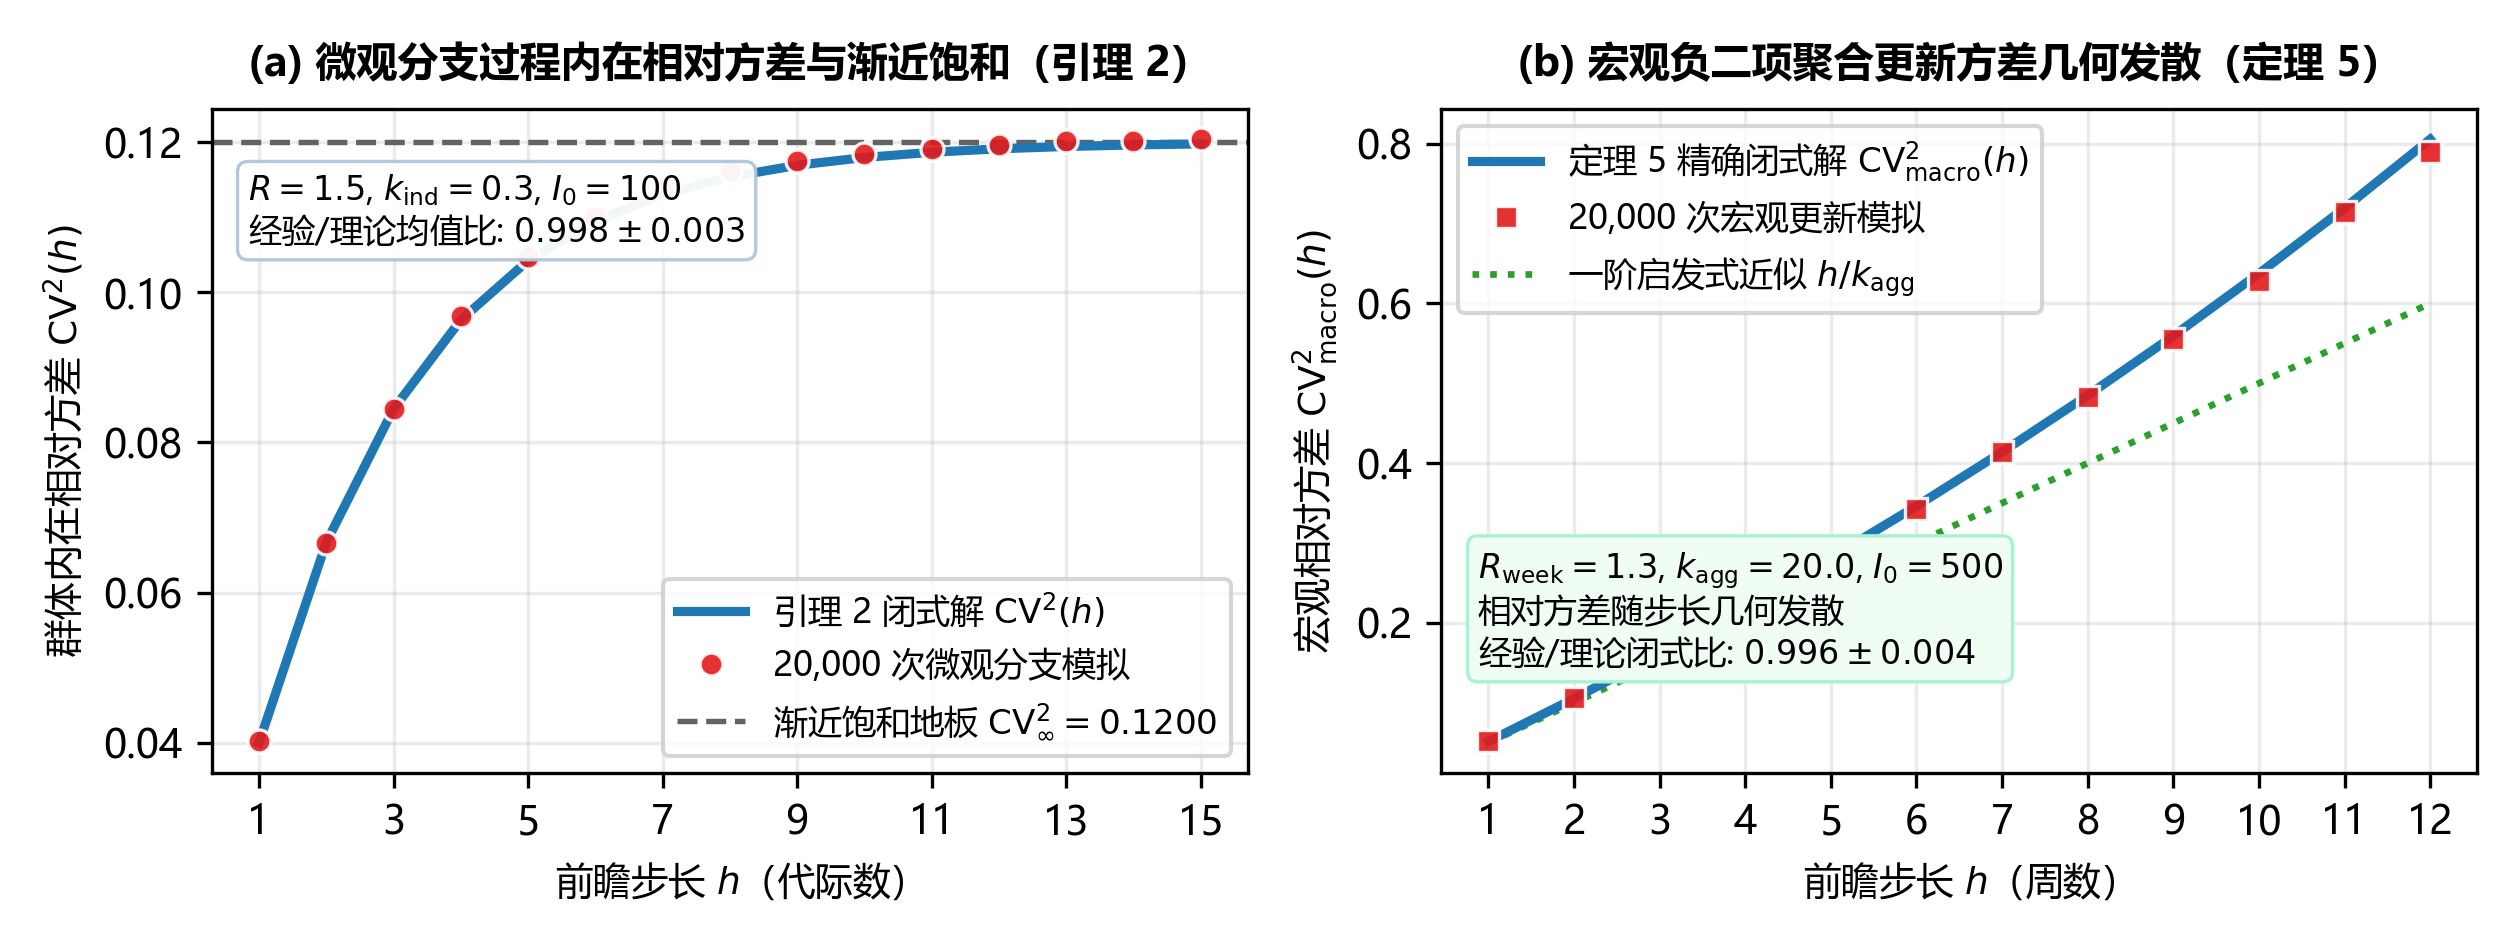
\includegraphics[width=\textwidth]{reports/figures_v2/fig2_cv_verify.png}
\caption{\textbf{微观分支方差饱和与宏观 NB2 更新方差几何增长的双尺度蒙特卡洛验证。}(a) 微观个体分支过程的相对方差饱和：在典型超临界传播设定下（$R=1.5, k=0.3, I_0=100$），蓝色实线为引理~\ref{lem:cv_floor} 闭式解 $\text{CV}^2(h)$，红色散点为 20,000 条独立模拟轨迹的经验统计，灰色虚线为渐近饱和值 $\text{CV}^2_\infty = 0.1200$；(b) 宏观 NB2 聚合更新模型的方差几何增长：在周度宏观更新设定下（$R_{\mathrm{week}}=1.3, k_{\text{agg}}=20, I_0=500$），蓝色实线为定理~\ref{thm:macro_exact} 精确闭式解，红色方块为 20,000 条模拟轨迹经验值，两者精确吻合；绿色点线为忽略空间二次项的一阶启发式近似 $h/k_{\text{agg}}$，在整个步长区间内持续低估（比值由 $h=1$ 的 0.970 单调降至 $h=12$ 的 0.745）。}
\label{fig:t1_verify_cn}
\end{figure}

\section{真实数据实证（上）：微观传播链与州级住院面板}\label{sec:empirical}

\subsection{监测数据来源、处理与分析窗口}\label{sec:data}

实证部分依托四层证据架构系统展开：第一层为理论模拟验证（第 4 节），后三层为真实数据实证，即个体传播链层（第 5.2 节）、州级住院面板层（第 5.3--5.5 节）与预测枢纽外部审计层（第 6 节）。各分析对象的参数来源、真值口径与数据架构详见补充材料附表 S3。

州级住院面板覆盖美国最多 51 个州级辖区（50 州加哥伦比亚特区）的三类主要呼吸道病原体：(1) COVID-19（Delta、Omicron、JN.1 三个波次）；(2) 季节性流感（2022--23、2024--25 流行季）；(3) 呼吸道合胞病毒 RSV（2024--25、2025--26 流行季）。分析统一使用周度新增确诊住院指标，不混合病例、检测与死亡目标。数据源自美国 CDC 数据门户终报冻结快照，统一了周度终报计数口径（早期 Delta 和 Omicron 住院数据经 HHS Protect 报告体系沉淀，后期由 NHSN 系统统一发布）。

数据预处理以各阶段起步期连续 5 个周度观测（$W=5$）作为基准推断窗口，采用对数线性回归估计周度增长乘子 $R_{\text{周}}=\exp(b_{\text{week}})$ 及其对数尺度标准误 $s_{\text{周}}=\text{SE}(b_{\text{week}})$（自由度 $\text{df}=3$）；由 Ho 等\citep{ho2023simultaneous} 对数差分二阶矩法估计宏观有效离散度 $k_{\text{agg}}$（设定上限 1,000）；初始发病规模 $I_0$ 取推断窗口内的周度均值。为保证参数推断的统计充分性与离散度的可识别性，数据筛选遵循通用准入准则：推断窗口（$W=5$ 周）内累计发病需达到 $\ge 50$ 例且各周均为非零正计数。该准则主要排除了低发病季节起步期的个别极小州（如早期阿拉斯加州、怀俄明州与佛蒙特州）及数据不连续的属地；各阶段最终纳入分析的辖区数为 26--51 个（详见表~\ref{tab:horizons} 与表~\ref{tab:budget_four}）。从样本选择效应看，该门槛必然系统性地剔除低发病起步期的辖区，而低计数单元恰好对应较小的 $I_0$ 与较大的 $\text{CV}^2_{\text{macro}}$，即机制视界最短的那部分单元；因此排除它们会向上偏置机制视界的测算值。由于该偏倚方向与本文"机制视界高于实测时效"这一结论的方向一致，本文不将其视为支持性证据，而按保守口径处理：表~\ref{tab:horizons} 的阶段中位视界应理解为可能被系统性\textbf{高估}的上界。为界定该偏倚的方向与幅度，第~\ref{sec:sensitivity} 节报告了将门槛放宽至 $\ge 20$ 例（及 $\ge 30$、$\ge 10$ 例）的敏感性分析。

关于 $I_0$ 取值口径，宏观更新模型 $Z_{t+1}\mid Z_t\sim\text{NB}(R_{\text{周}}Z_t,k_{\text{agg}})$ 的马尔可夫理论起点应为即时状态 $Z_t$；本文采用 5 周窗口均值 $\bar Z$ 是为平滑观测噪声。敏感性分析表明，将 $I_0$ 分别设定为窗口均值、末周计数与对数拟合末端值时，各阶段州级中位机制视界的变化仅在 $-0.2\%\sim +4.8\%$ 之间（个别低计数州最大变动约 $+51\%$），整体对主口径结论保持稳健。若改用小样本 $t(3)$ 临界值替换渐近标准正态分位数，区间宽度相应扩大 1.62 倍（见第 5.6 节讨论）。

\subsection{微观传播链层：子代分布与信息论下界的个体级验证}\label{sec:micro}

微观个体层面分析基于两组权威公开的接触追踪数据集：中国香港 COVID-19 早期传播网络（本地聚集性子队列 $N=355$ 与全队列 $N=1,038$）\citep{adam2020clustering}，以及几内亚科纳克里埃博拉传播网络（$N=152$）\citep{faye2015chains,althaus2015ebola}。其中香港本地子群排除了输入性散发个案，聚焦于本土社区微观传播链；全队列则包含完整输入与二代病例。对各数据集实施负二项极大似然拟合，并以 Poisson 分布作为零假设基准（表~\ref{tab:micro} 与图~\ref{fig:micro}）：

\begin{table}[htbp]
\centering
\footnotesize
\caption{微观传播链层的子代分布极大似然拟合与信息论下界检验}\label{tab:micro}
\setlength{\tabcolsep}{3pt}%
\begin{tabular}{lcc c c c cc c c}
\toprule
数据集 & $N$ & $\hat R$ & 95\% CI & $\hat k$ & 95\% CI & 经验 $\text{CV}^2$ & 理论 $\text{CV}^2$ & $\Delta\text{AIC}$ & 自助/CRB \\
\midrule
Hong Kong COVID19 Local & 355 & 0.473 & 0.37--0.58 & 0.434 & 0.30--0.71 & 5.46 & 4.42 & 93.9 & 1.059 \\
Hong Kong COVID19 All & 1038 & 0.162 & 0.13--0.20 & 0.111 & 0.08--0.16 & 17.85 & 15.19 & 223.4 & 1.027 \\
Guinea Ebola 2014 & 152 & 0.954 & 0.61--1.36 & 0.182 & 0.12--0.30 & 6.41 & 6.56 & 244.0 & 0.984 \\
\bottomrule
\end{tabular}

\end{table}

\begin{figure}[htbp]
\centering
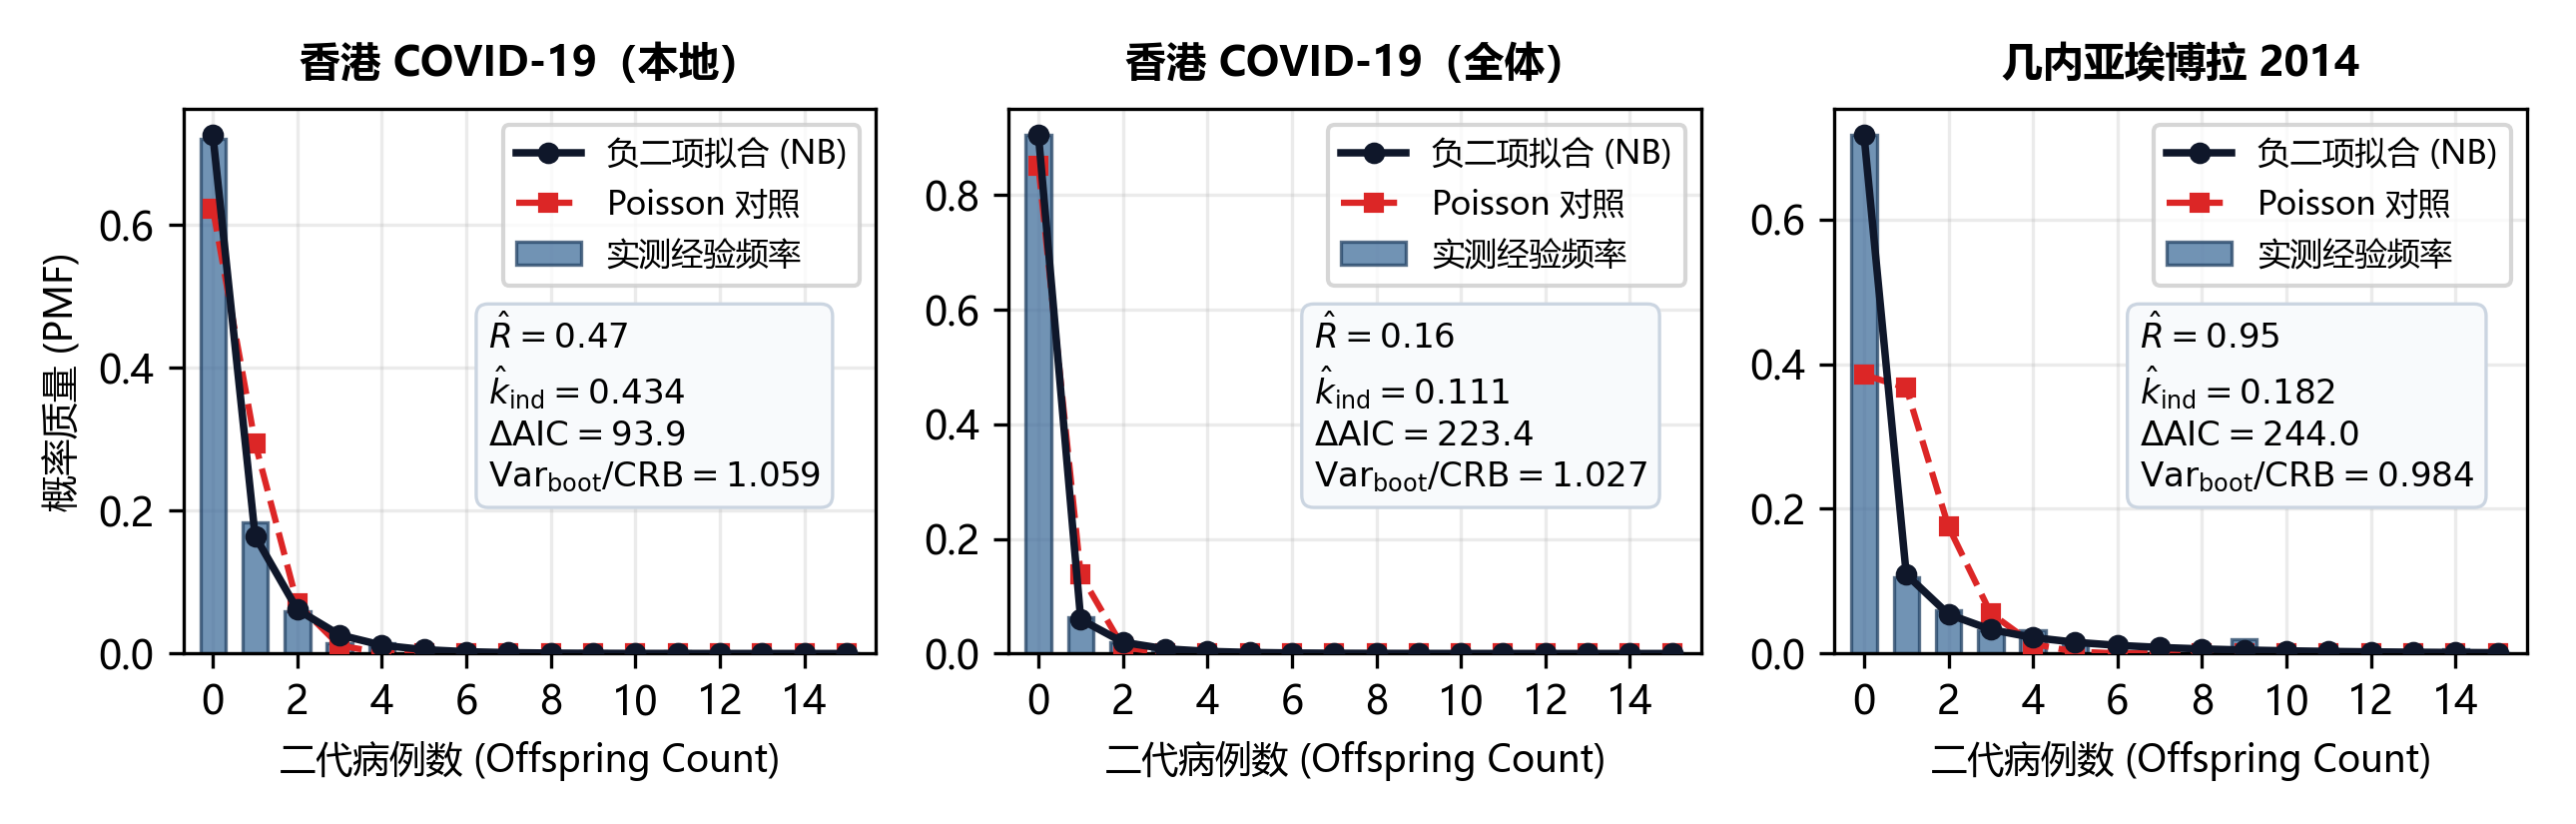
\includegraphics[width=\textwidth]{reports_v3/figures/fig_micro.png}
\caption{\textbf{个体传播链子代分布的负二项拟合与 Cramér--Rao 下界验证。}香港本地子群（左）、香港全队列（中）与几内亚埃博拉（右）三组权威接触追踪数据的极大似然 PMF 拟合（柱状为实测经验频率，深色实线散点为负二项拟合，红色虚线为 Poisson 对照）。标注框列出参数估计（$\hat{R}, \hat{k}$）、$\Delta\text{AIC}$ 拟合优度差距（$\Delta\text{AIC} = 93.9\text{--}244.0$，显示负二项模型具有显著更优的拟合表现）以及参数化 Bootstrap 方差与 Cramér--Rao 下界效率比（$\text{Ratio} \in [0.984, 1.059]$），表明负二项参数化设定下的数值 MLE 方差与 Fisher 信息解析计算精确吻合。}\label{fig:micro}
\end{figure}

实证分析揭示了两个关键特征：
第一，三组微观传播链数据均表现出强烈的过度离散现象。负二项模型相对于 Poisson 模型的 AIC 优势显著（$\Delta\text{AIC}$ 达 93.9--244.0）。香港全队列与几内亚埃博拉的实测离散参数分别低至 $\hat{k} = 0.111$ 与 $0.182$\citep{althaus2015ebola}，表明超级传播事件与高度异质性是微观动力学的固有特征。
第二，经验参数估计效率严格遵循定理~\ref{thm:fisher} 的理论预期。参数化 Bootstrap 方差与 CRB 之比在三组数据中分别为 1.059、1.027 与 0.984（位于 0.984--1.059 区间），在蒙特卡洛抽样误差范围内与理论下界高度吻合。这一分析确立了负二项参数化在微观尺度的经验有效性，并为基于 Fisher 信息量纲反解早期参数辨识的数据充分性门槛（定理~\ref{thm:fisher}）与视界标度（推论~\ref{cor:crb_horizon}）提供了经验锚点。

\subsection{州级面板层：NB2 模型内机制视界的空间分布与聚合效应}\label{sec:state_panel}

\noindent\textbf{视界口径界定。}全文涉及四种不同视界概念（详见补充材料附表 S4 对照表）。本文的州级主分析对象为\textbf{插件式 NB2 模型内机制视界}（简记为 NB2 机制视界），即在固定 $k_{\text{agg}}$ 插件估计条件下、由定理~\ref{thm:macro_exact} 的精确有限步方差方程确定的理论阈值根。

将宏观 NB2 方差方程应用于州级面板（覆盖最多 51 个州级辖区，各阶段起步期 5 周推断窗口；$k_{\text{agg}}$ 由对数差分二阶矩估计，$R$ 与 $s$ 为对数线性回归参数），得到各阶段各辖区的 NB2 机制视界分布（表~\ref{tab:horizons} 与图~\ref{fig:state_horizons}）。宏观更新模型的方差递推含 $Z_{t-1}^2$ 二次项并以 $(1+1/k_{\text{agg}})^h$ 几何增长，与微观分支的渐近饱和形成对照；若将微观分支闭式直接启发式套用于宏观序列，会将模型内相对方差低估 3.7--31.7 倍（见补充材料附表 S5）。

三项结果值得强调。第一，\textbf{在七个阶段中，有六个阶段的州级中位数低于国家级聚合序列的对应视界}：Delta 阶段州级中位视界 7.1 周对国家级 17.0 周，流感 2022--23 为 2.2 周对 6.3 周，RSV 2024--25 为 5.8 周对 38.1 周。关于适用域闸门：假设 (A2) 要求 $R$ 在预测视界内恒定，而两季 RSV 的国家级 $h^*$ 分别为 38.1 与 60.4 周，按表~\ref{tab:horizons} 自身参数折合 $R^{h_{\text{gen}}}$ 达 $2.1\times10^4$ 与 $1.9\times10^6$ 倍，其中 RSV 2025--26 的预测周发病量已达 $3.5\times10^9$，超过美国总人口，越出分支近似的有效域；表~\ref{tab:horizons} 因此将这两个国家级测算值记作 $\ge 20$（单流行季跨度）而不作为可操作指标，而 Delta 国家级 17.0 周落在单季 20 周跨度内，按实际值列报。逐州符号检验显示，七个阶段中有六个阶段的大多数辖区视界短于国家级（Delta 42/50、JN.1 35/51、两季流感 32/38 与 39/45、两季 RSV 34/34 与 26/26），仅 Omicron 例外（25/51，与国家级 3.9 周不可区分）。需要指出，各州受共同季节与毒株驱动存在强空间相关，且国家级为各州之和，故该计数仅作方向性描述而非独立显著性证据。机制上，州级序列斜率标准误 $s$ 整体高于国家级，宏观聚合的平滑效应抬高了视界。进一步复算表明，宏观过程方差在视界工作点处占主导：$\text{CV}^2_{\text{macro}}(h^*)/\tau^2$ 跨州中位数达 $0.73$--$0.89$，即宏观过程离散度构成了州级视界的核心约束。此外，RSV 2025--26 仅 26 个州、流感 2022--23 仅 38 个州满足数据门槛，从经验上说明低计数阶段更容易受到数据充分性限制，但不能视为对定理~\ref{thm:fisher} 个体级样本量界的直接验证。

\noindent\textbf{口径边界与方差结构敏感性。}州级主口径严格界定为\textbf{插件式 NB2 模型内机制视界}，其中 $k_{\text{agg}}$ 由 5 周短滑动窗口约 4 个周度对数差分估计，仅作为有效时序离散度代理参数。式~\eqref{eq:macro_cv2_closed} 中的几何项 $[(1+1/k_{\text{agg}})^h-1]$ 是 NB2 二次过度离散结构的内生产物，因而 2.2--7.1 周的有限机制视界具有明确的模型依赖性：
(1) \textbf{替代宏观方差结构的理论敏感性}：若改用纯 Poisson 更新模型（$k_{\text{agg}}\to\infty$），则在 $R>1$ 时宏观过程相对方差由零单调增加并饱和于 $1/[I_0(R-1)]$（式~\eqref{eq:poisson_cv2_limit}），在 $R=1$ 时呈线性累积，不再呈 NB2 式几何增长；若采用 NB1 或准 Poisson 结构（方差 $\phi \mu$），在超临界条件下相对方差同样有界饱和，在近临界条件下呈线性累积，均不产生固定离散度 NB2 结构中的几何增长项。但完整插件式风险还包含随步长发散的参数外推项 $P_{\text{exact}}(h; s)$，因此替代模型下的机制视界仍须在保留相同参数项后重新求根比较，不能仅根据过程方差的渐近饱和判定为无界。对数残差关于发病规模的经验散点显示方差可能随规模超线性增加，为采用 NB2 作为基准工作模型提供了初步描述性支持，但尚不足以证明 NB2 优于 NB1、动态离散度或状态空间模型。
(2) \textbf{预设多窗口结果范围（窗口选择敏感性范围）}：针对滑动窗口长度选择所带来的结构不确定性，本文报告 $W \in \{5, 6, 8, 10\}$ 四种预设窗口下视界点估计的极值范围 $\mathcal{R}_W \equiv [\min_{W} \hat{h}^*(W), \max_{W} \hat{h}^*(W)]$（详见补充材料附表 S6）：COVID Delta 为 $[6.79, 8.07]$ 周、Omicron 为 $[3.61, 4.17]$ 周、JN.1 为 $[4.24, 7.23]$ 周、流感 2022--23 为 $[1.79, 2.39]$ 周、流感 2024--25 为 $[1.52, 3.03]$ 周、RSV 2024--25 为 $[2.98, 6.21]$ 周、RSV 2025--26 为 $[3.89, 5.58]$ 周。该范围仅反映四种预设推断窗口选择之间的结构敏感性，不具有统计置信区间性质，也不传播各窗口内部的参数估计抽样不确定性。各阶段中位视界在窗口变换下出现 $-48.7\%$ 至 $+44.6\%$ 浮动，反映了样本量增加降低估计标准误与引入非平稳均值漂移之间的结构权衡。
(3) \textbf{其他敏感性}：$k_{\text{agg}}$ 截断上限对多数 COVID 阶段及流感 2024--25 影响极小（100 与 1000 上限之间差异低于 $0.3\%$）；在流感 2022--23 及两季 RSV 中，100 与 1000 上限之间的中位视界差异为 $3.4\%\text{--}7.4\%$（若以 100 上限为基准对比无约束 $\infty$ 则为 $3.3\%\text{--}8.1\%$），仍显著小于推断窗口长度引起的变化，但不能概括为所有阶段均低于 $0.3\%$；$I_0$ 初值口径变动影响在 $-0.2\%\sim +4.8\%$ 之间；偏差修正预测使视界微弱延长 $0.3\%$--$1.5\%$。

补充材料附表 S5 给出六个视界口径与实测时效的完整对照。插件式 NB2 模型内机制视界的州级中位数（2.2--7.1 周，多窗口范围覆盖 1.52--8.07 周）在全部七个阶段均高于同定义实测绝对视界（阶段级中位数之比为 1.11--4.00 倍；逐州严格配对的中位比为 1.79，见第~\ref{sec:rolling_eval} 节）。但若代入极端个体级微观离散度（$\hat{k}=0.111$），低计数阶段视界可降至实测之下。因此主结论严格界定为：主结果成立于插件式宏观 NB2 口径（机制视界高于实测绝对时效）；中等个体离散度的微观映射仅提供平行敏感性对照。“宽松包络”应理解为该特定模型设定下的诊断性经验参考基准，而非现实预测系统的绝对物理上限。

\begin{table}[htbp]
\centering
\footnotesize
\caption{州级面板各阶段动力学参数与插件式 NB2 模型内机制视界分布（中位数与四分位距）}
\label{tab:horizons}
\setlength{\tabcolsep}{3pt}%
\begin{tabular}{lccccccc}
\toprule
阶段 & $n_{\text{州}}$ & $R$ 中位数 [IQR] & $s$ 中位数 & $k_{\text{agg}}$ 中位数 & $I_0$ 中位数 & $h^*_{\text{周}}$ 中位数 [IQR] & 国家级 $h^*_{\text{周}}$ \\
\midrule
COVID-19 Delta 暴发期 & 50 & 1.175 [1.134, 1.228] & 0.0250 & 56.6 & 297 & 7.1 [3.4, 12.1] & 17.0 \\
COVID-19 Omicron 达峰期 & 51 & 1.041 [0.987, 1.101] & 0.0206 & 21.0 & 757 & 4.0 [2.5, 8.0] & 3.9 \\
COVID-19 JN.1 流行期 & 51 & 1.022 [0.998, 1.047] & 0.0223 & 29.5 & 391 & 5.0 [3.8, 7.8] & 7.0 \\
流感 2022--23 暴发早期 & 38 & 1.223 [1.167, 1.333] & 0.0332 & 11.2 & 55 & 2.2 [1.0, 4.6] & 6.3 \\
流感 2024--25 流行季 & 45 & 1.241 [1.201, 1.293] & 0.0291 & 17.4 & 96 & 2.6 [1.8, 7.1] & 11.1 \\
RSV 2024--25 流行季 & 34 & 1.430 [1.341, 1.522] & 0.0520 & 39.8 & 76 & 5.8 [2.6, 10.1] & $\ge 20^{\dagger}$ \\
RSV 2025--26 流行季 & 26 & 1.372 [1.274, 1.444] & 0.0655 & 23.7 & 37 & 3.9 [1.4, 9.1] & $\ge 20^{\dagger}$ \\
\bottomrule
\end{tabular}
%
\vspace{2pt}
\begin{flushleft}
\scriptsize \textbf{注：}每行统计通过数据门槛（窗口累计 $\ge 50$ 例且每周非零）的州级辖区。全部参数在周度时钟上定义：$R_{\text{周}}=\exp(b_{\text{week}})$ 为周度增长乘子，$s_{\text{周}}=\text{SE}(b_{\text{week}})$ 为对数标准误（$\text{df}=3$）；$k_{\text{agg}}$ 为对数差分二阶矩估计（预设上限 1,000，共有 6.4\% 的州—阶段估计触及上限。对于这些单元，相对于可能更大的无约束估计值，截断到 1,000 会略微增加 NB2 过程方差并缩短视界；但其整体仍接近 Poisson 极限，且该截断对阶段中位数的影响较小，详见第 5.3 节与第 5.6 节）；$I_0$ 为窗口周度均值；$h^*_{\text{周}}$ 为插件式 NB2 模型内全方差临界方程（$\tau=0.5$、精确参数外推项 $P_{\text{exact}}(h)$）通过全方程数值求得的连续阈值根（NB2 模型内机制视界主口径）；末列为 51 个州级辖区聚合的国家级序列对应值。$\dagger$ 标注表示国家级测算值超出单季 20 周跨度（记作 $\ge 20$）。代间隔 $\mu_g$ 仅用于微观尺度映射，不进入本表主口径计算。\end{flushleft}
\end{table}

\begin{figure}[htbp]
\centering
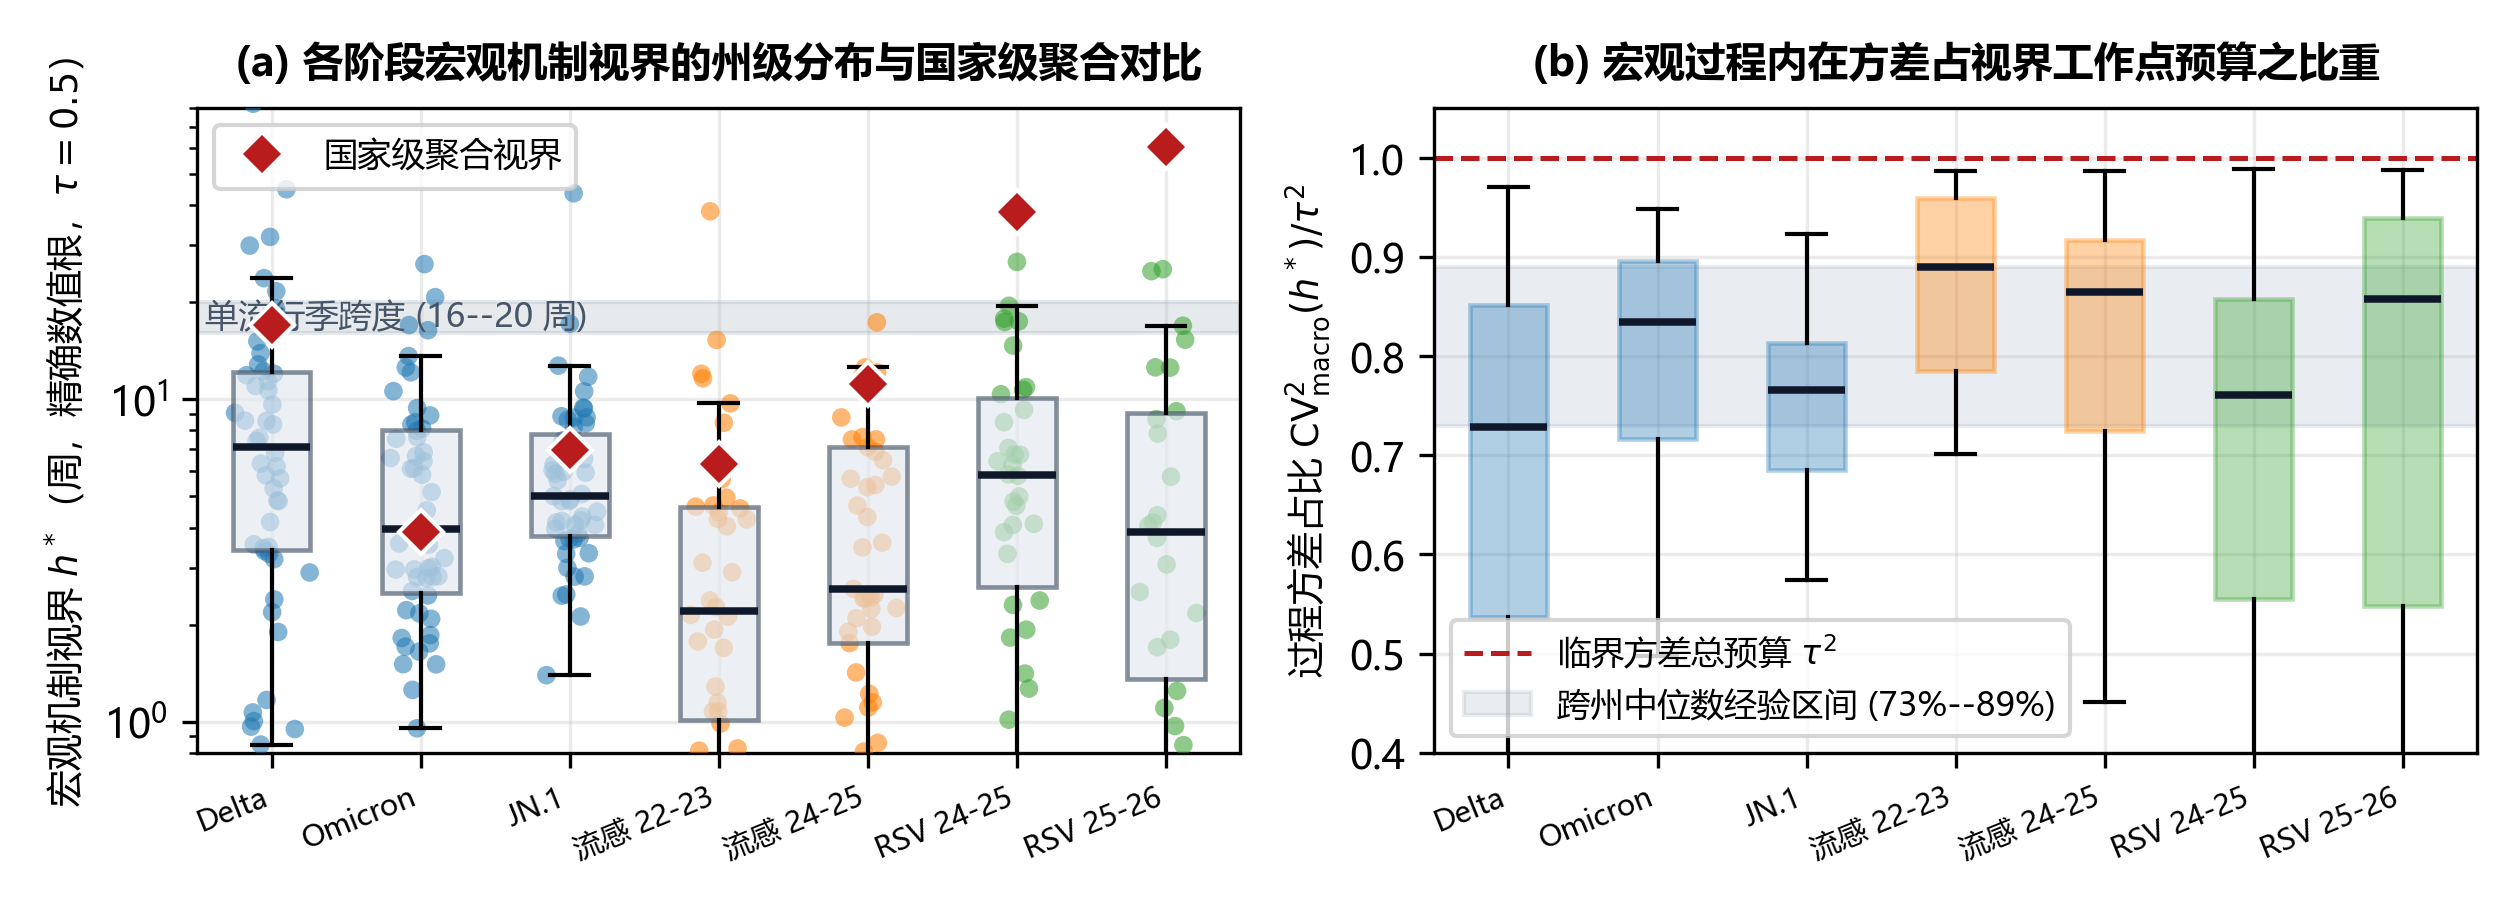
\includegraphics[width=\textwidth]{reports_v3/figures/fig_state_horizons.png}
\caption{\textbf{NB2 模型内机制视界的州级分布、国家级聚合值对比与方差主导比率。}(a) 各流行阶段州级辖区插件式 NB2 模型内机制视界 $h^*_{\text{exact}}$（周，对数纵轴）的箱线图与抖动散点分布（按病原体着色），红色空心菱形为 51 个州级辖区求和的国家级序列视界。国家级值在七个阶段中的六个高于州级中位数（唯一例外是 Omicron），展示空间聚合平滑对机制视界的抬升；(b) 视界临界工作点处的宏观过程方差主导比率 $\text{CV}^2_{\text{macro}}(h^*)/\tau^2$，跨阶段中位数稳定在 0.73--0.89，表明宏观过程离散度构成了州级机制视界的核心刚性约束。灰色带标示呼吸道病毒单流行季 16--20 周的自然跨度。}
\label{fig:state_horizons}
\end{figure}

\noindent\textbf{宏观方差结构本身是视界的主要依赖来源。}上述全部结果都在固定离散度的 NB2 宏观更新模型下取得，而其相对过程方差含几何项 $(1+1/k_{\text{agg}})^h$。为一个结构的成立与否划定边界，表~\ref{tab:alt_variance} 在\textbf{同一州级面板、同一 5 周推断窗口、同一参数集与同一容忍度 $\tau=0.5$}下比较四种宏观方差结构下的机制视界：(i) 主口径 NB2 固定 $k_{\text{agg}}$；(ii) 线性过度离散的 NB1／准 Poisson（$Var=\phi R Z_t$，其中 $\phi$ 校准为使单步条件方差在工作点 $\mu=I_0$ 处与 NB2 相等，$\phi=1+R I_0/k_{\text{agg}}$，故差异纯属结构而非尺度）；(iii) Poisson 更新（$\phi=1$）；(iv) 微观 Galton--Watson 口径在 $k_{\text{agg}}$ 处取值。结果显示：\textbf{由 NB2 换成 Poisson 后，各阶段中位视界由 2.20--7.12 周延长至 5.07--11.10 周（约 2.0 倍）}，NB1 居中（2.93--9.34 周）。机制在闭式上是清楚的——NB1 与 Poisson 的相对过程方差为 $\phi\,(1-R^{-h})/[I_0(R-1)]$，随 $h$ \textbf{饱和}；而 NB2 的几何项由 $h\approx 3$ 起开始支配，正是本文视界偏短的直接来源。

因此，本文报告的 2.2--7.1 周不是数据自身给出的视界，而是"固定离散度 NB2 工作模型 $+$ 周度时钟 $+$ 插件参数"三者的联合产物；在结构上更接近 Poisson 或 NB1 的宏观更新模型下，换用 Poisson 结构后各阶段中位视界延长为 1.56--2.56 倍（跨阶段均值约 1.96 倍）；换用 NB1／准 Poisson 结构亦延长为 1.06--1.53 倍（均值 1.27 倍）。该量级显著超过 $k_{\text{agg}}$ 上限截断（$\le 7.4\%$）与推断窗口长度（$\pm 45\%$）所引起的变化，故应被视为首要的结构性不确定性来源，而非次要的稳健性细节。

\begin{table}[htbp]
\centering
\footnotesize
\caption{同一州级面板与同一参数集下，四种宏观方差结构给出的机制视界（周，跨州中位数）}
\label{tab:alt_variance}
\begin{tabular}{lcccc}
\toprule
阶段 & NB2 固定 $k$ & NB1／准 Poisson & Poisson & 微观 GW 口径 \\
\midrule
COVID-19  & 7.12 & 9.34 & 11.10 & 11.08 \\
COVID-19  & 3.95 & 5.12 & 8.57 & 8.57 \\
COVID-19  & 5.00 & 5.29 & 9.34 & 9.31 \\
流感 2022-- & 2.20 & 2.93 & 5.07 & 5.02 \\
流感 2024-- & 2.58 & 3.95 & 6.60 & 6.59 \\
RSV 2024- & 5.82 & 7.46 & 9.55 & 9.54 \\
RSV 2025- & 3.89 & 4.66 & 6.32 & 6.29 \\
\bottomrule
\end{tabular}

\end{table}

\subsection{三项描述性误差记账与模型—观测代数差额}\label{sec:budget}

按差额定义 $\mathcal{E}_{\text{res}}(h)$ 后，三项误差记账架构在州级面板上逐州逐阶段执行，构建如下描述性代数记账恒等式（表~\ref{tab:budget_four}）：
\begin{equation}
\text{RelMSE}_{\text{obs}}(h) = \text{CV}^2_{\text{macro}}(h) + P_{\text{quad}}(h) + \mathcal{E}_{\text{res}}(h).
\label{eq:full_budget}
\end{equation}
各分量口径与前文保持自洽：$\text{CV}^2_{\text{macro}}(h)$ 取自定理~\ref{thm:macro_exact} 式~\eqref{eq:macro_cv2_closed}，代表固定离散度宏观更新模型的条件精确有限步相对方差；参数外推项 $P_{\text{quad}}(h) = (h_{\text{周}} s_{\text{周}})^2$ 是 $P_{\text{exact}}(h)$ 在领先阶上的二次项，刻画斜率估计不确定性的确定性传播；实测总相对误差 $\text{RelMSE}_{\text{obs}}(h)$ 由各州在滚动预测原点上在线评估求得；$\mathcal{E}_{\text{res}}(h)$ 定义为模型—观测代数差额（Model-Observation Algebraic Discrepancy）。关于漂移项，时变漂移代理 $\mathcal{E}_{\text{drift}}(h) = h_{\text{周}}\widehat{v}^2_{\text{周}}$ 因小样本因果估计的波动性未纳入主记账恒等式，作为有界敏感性分析单独报告（表注）。

式~\eqref{eq:full_budget} 构建了一套自洽的实测误差分解记账框架。实测均方误差基于样本外滚动预测在线评估生成，而理论方差分量来自机制动力学与时序离散度模型设定。在现实流行过程中，由于外生干预、报告延迟与时变漂移的存在，实测误差与模型内生方差之间存在天然的结构性偏离。因此，差额项 $\mathcal{E}_{\text{res}}(h)$ 定量刻画了理想化机制模型与真实业务复杂系统之间的\textbf{经验建模赤字（Empirical Modeling Deficit）}，其主要构成涵盖：(1) 行为自适应与非药物干预引发的动态漂移；(2) 医疗报告系统的回填与修订；(3) 统计模型形式设定的结构简化；(4) 参数外推领先阶近似 $P_{\text{quad}}$ 在有限步长内的微弱低估（在 $h=4$ 处约低估 4\%--16\%）：
\begin{equation}
\mathcal{E}_{\text{res}}(h) \equiv \text{RelMSE}_{\text{obs}}(h) - \left[ \text{CV}^2_{\text{macro}}(h) + P_{\text{quad}}(h) \right].
\end{equation}

误差记账的实测分解表明：机制方差与参数外推项占实测总均方误差的比例在不同阶段为 $4.2\%\sim 100\%$，而模型—观测代数差额在全部 21 个阶段--步长配置中的跨州中位占比中位数为 $55.0\%$（其中 $h=1$ 步长在 7 个阶段的中位数为 $45.4\%$，随步长延伸上升至 $h=4$ 的 $78.6\%$）。在当前工作模型设定下，显式计算的宏观过程方差与参数外推项在多数配置中不足以覆盖实测误差，差额项综合吸收了非平稳漂移与现实报告扰动。这表明理论机制视界应被理解为基于动力学生成假设的“现实预警时效的经验参考外包络”，而非现实业务系统的紧致预测极限。

州级分解的具体测算结果如下。\textbf{模型—观测代数差额的跨州中位占比在全部 21 个阶段--步长配置中介于 $-0.0\%$--$95.8\%$（中位 $55.0\%$）}：Delta 阶段由 $h=1$ 的 60.6\% 升至 $h=4$ 的 95.8\%，Omicron 为 32.0\%--78.6\%，JN.1 为 $-0.0\%$--31.1\%，流感 2022--23 为 45.4\%--81.5\%，流感 2024--25 为 55.0\%--86.9\%，RSV 2024--25 为 47.9\%--59.5\%，RSV 2025--26 为 10.8\%--15.2\%。\textbf{为正占比}：各阶段--步长配置中，代数差额为正的州占比介于 49\% 与 94\% 之间。\textbf{两项已建模分量的量级符合理论预期}：在 NB2 插件式口径下，$\text{CV}^2$ 在视界工作点处成为主导分量（$\text{CV}^2_{\text{macro}}(h^*)/\tau^2$ 的跨州中位数 0.73--0.89，见第 5.3 节），参数项 $P_{\text{quad}}$ 随 $h^2$ 增长；例如 Delta 在 $h=4$ 时 $\text{CV}^2$ 中位 $981.6\times10^{-4}$、$P_{\text{quad}}$ 中位 $222.4\times10^{-4}$，对应跨州中位数口径下，二者之和约为实测总误差中位数 $34744\times10^{-4}$ 的 3.5\%。

\begin{table}[htbp]
\centering
\footnotesize
\caption{两项显式模型分量与模型—观测代数差额的描述性误差记账州级分解（各分量绝对值 $\times 10^{-4}$ 的中位数与代数差额占比分布）}
\label{tab:budget_four}
\setlength{\tabcolsep}{3pt}%
\begin{tabular}{lcccccc}
\toprule
& \multicolumn{3}{c}{$h = 1$ 周前瞻} & \multicolumn{3}{c}{$h = 4$ 周前瞻} \\
\cmidrule(lr){2-4}\cmidrule(lr){5-7}
阶段名称 & $\text{RelMSE}_{\text{obs}}$ & 闭合残差占比 & 为正占比 & $\text{RelMSE}_{\text{obs}}$ & 闭合残差占比 & 为正占比 \\
\midrule
COVID-19 Delta 暴发期    & 626.9  & 60.6\% [25.3, 78.6]  & 86\% & 34744.0 & 95.8\% [87.2, 98.3] & 94\% \\
COVID-19 Omicron 达峰期  & 816.8  & 32.0\% [16.4, 48.4]  & 92\% & 8165.2  & 78.6\% [48.8, 90.2] & 90\% \\
COVID-19 JN.1 流行期     & 332.3  & -0.0\% [-36.0, 18.2] & 49\% & 2602.2  & 31.1\% [5.8, 55.9]  & 78\% \\
流感 2022--23 暴发早期   & 1828.3 & 45.4\% [24.0, 72.9]  & 87\% & 23754.5 & 81.5\% [42.1, 95.9] & 87\% \\
流感 2024--25 流行季     & 1458.9 & 55.0\% [24.4, 72.4]  & 84\% & 20689.3 & 86.9\% [68.3, 97.5] & 89\% \\
RSV 2024--25 流行季      & 696.5  & 47.9\% [-10.7, 72.8] & 74\% & 3872.4  & 59.5\% [30.6, 76.7] & 79\% \\
RSV 2025--26 流行季      & 760.1  & 15.2\% [-1.1, 53.2]  & 69\% & 3019.9  & 13.1\% [-50.3, 64.2]& 54\% \\
\bottomrule
\end{tabular}%
\vspace{2pt}
\begin{flushleft}
\scriptsize \textbf{注：}每行统计通过数据门槛的州级辖区（$n_{\text{州}}$ 列）；各分量列报跨州中位数（单位 $10^{-4}$）；代数差额占比列为跨州中位数及四分位距，末列为代数差额为正的州占比。实测总误差由各州滚动原点（$W=4$ 在线重估）计算，模型—观测代数差额按 $\mathcal{E}_{\text{res}} = \text{RelMSE}_{\text{obs}} - (\text{CV}^2_{\text{macro}} + P_{\text{quad}})$ 吸收定义。因各列为跨州独立取中位数，各分量中位数之和在代数上不等于实测总误差中位数。时变漂移代理 $\mathcal{E}_{\text{drift}} = h_{\text{周}}\widehat{v}^2_{\text{周}}$ 因小样本因果估计不稳健未纳入主恒等式，在 $h=4$ 处量级为 $0.21$--$1.27$（与实测同阶），主恒等式以不含漂移的三项口径为准。\end{flushleft}
\end{table}

\subsection{伪实时滚动回测：多州样本外技能衰减与双层对照}\label{sec:rolling_eval}

滚动回测在最多 51 个州级辖区上独立展开。对每个州，模型以 $W=4$ 周滑动窗口在 6 个逐周原点上在线重估对数斜率，向前生成 $h=1,\dots,8$ 周点预测，并与持续性基线及局部线性基线展开平行对照。对各州分别计算跨原点的均方误差比值：
\begin{equation}
\text{MSERatio}_{i}(h) = \frac{\text{MSE}_{i,\text{model}}(h)}{\text{MSE}_{i,\text{base}}(h)}, \quad \text{MSE}_{i,m}(h) = \frac{1}{6}\sum_{o=1}^{6}\left(\frac{\hat{y}_{i,m,o,h} - y_{i,o,h}}{z_{i,o}}\right)^2,
\end{equation}
其中下标 $i$ 表示州，$o$ 为预测原点，$h$ 为前瞻步长，$z_{i,o}$ 为原点观测水平。通过求解比率曲线穿越 1.0 的插值交叉点，确定各州的业务时效边界，并汇总其跨州分布（表~\ref{tab:rolling}）。鉴于该穿越点基于 6 个原点插值求得，本文采用跨州中位数与四分位距刻画其空间离散性，并通过 2,000 次原点级自助重抽量化其抽样不确定性。

州级回测结果显示出清晰的技能衰减规律：相对持续性基线的州级中位穿越点为 Delta 3.7 周（IQR 2.9--5.0）、Omicron 1.4 周、JN.1 1.0 周、流感 2022--23 2.8 周、流感 2024--25 2.9 周、RSV 2024--25 1.3 周、RSV 2025--26 4.3 周，整体落在 1.0--4.3 周区间；国家级对应值分别为 3.52、1.82、1.00、5.34、4.10、1.57 与未穿越（落在 1.0--5.3 周）。相对局部线性基线的州级列给出的是 MSE 比自上方下穿 1.0 的插值步长，七个阶段的中位下穿点为 1.0--1.2 周。两类基线的穿越方向具有不同的评估含义：相对持续性基线上穿 1.0 代表外推模型相较朴素持续性的预测技能丧失（中位数 1.0--4.3 周）；相对局部线性基线下穿 1.0 则表明模型在最短步长附近即已追平局部线性外推（约 1 周），在更长步长处两者表现趋于一致。

关于穿越点的估计不确定性：对每个州以 6 个逐周原点作原点级自助重抽（$B=2{,}000$），州级中位穿越点的 95\% 自助区间为：相对持续性基线 $[1.0, 6.8]$ 周（逐阶段中位区间的下界恒为 1.0 周，上界 3.3--6.8 周），相对局部线性基线 $[1.0, 5.1]$ 周。区间跨度与 6 个原点的小样本规模相符，因此“1.0--4.3 周”体现为跨阶段的点估计经验范围。

在绝对误差维度下，按照相对均方根误差首次达到 $\tau = 0.5$ 的同一定义，各阶段实测绝对误差视界的州级中位数为 1.2--3.9 周（表~\ref{tab:rolling} 第 5 列）。与表~\ref{tab:horizons} 中的 NB2 机制视界相比，各阶段汇总中位数之比显示机制视界约为实测绝对视界的 1.11--4.00 倍。需要说明：该比值是两个阶段级中位数之比，而表~\ref{tab:horizons} 与表~\ref{tab:rolling} 的准入规则不同（前者要求推断窗口累计 $\ge 50$ 例且各周非零，后者要求回测窗口累计 $\ge 30$ 例），同一阶段的参与州集合并不相同（如 RSV 2024--25 为 34 对 43 州），故中位数之比不具备配对解释；下段给出在同一辖区上严格配对的逐州比值。

为直接检验汇总中位数之比是否掩盖了州级异质性，本文在同一辖区上同时计算机制视界与实测视界，构造逐州配对比 $\text{Ratio}_i \equiv h^{*}_i / h^{\text{obs}}_i$（$h^{\text{obs}}_i$ 由该州自身的滚动原点、以同一容忍度 $\tau=0.5$ 在周度网格上插值求得）。在准入准则下共 294 个辖区—阶段单元得到可解析的实测视界（1 个单元在网格内始终未穿越 $\tau$，按删失处理并如实报出）。配对结果显示：Delta 中位比 3.76（IQR [1.77, 6.78]）、Omicron 1.84（[1.46, 3.03]）、JN.1 1.31（[1.03, 1.66]）、流感 2022--23 与 2024--25 分别为 1.43（[0.82, 2.56]）与 2.43（[1.22, 3.67]）、RSV 2024--25 与 2025--26 分别为 1.86（[1.44, 3.24]）与 1.16（[0.69, 2.23]）；全样本 294 个单元的中位比为 1.79（IQR [1.10, 3.36]），其中 \textbf{78.9\%} 的单元比值大于 1、\textbf{21.1\%} 小于 1（精确符号检验 $p < 10^{-15}$，但该检验假设单元独立，与第~\ref{sec:limitations} 节所述州级强空间相关相抵触，故仅作参考而不作为显著性主张）。这一结果需要如实解读：\textbf{配对比的中位大于 1 是分布中心的性质，而非逐点占优的性质}——在流感 2022--23 与 RSV 2025--26 两阶段分别有 31.6\% 与 38.5\% 的辖区比值低于 1，且这两阶段的四分位下界亦低于 1。因此本文的准确表述是：机制视界在多数（约八成）州级单元上构成实测绝对时效的外包络，但该外包络并非逐点成立，在低计数阶段存在约三分之一的系统性反号单元；上文"宽松经验参考外包络"的定位应理解为对分布中心的描述。逐州配对（中位 1.79）与阶段汇总中位数之比（1.11--4.00）在量级上一致，二者互为交叉印证。

双层对照清晰地划分了两类实测时效的物理含义：按同一容忍度 $\text{RelRMSE} \le 0.5$ 定义的实测绝对误差视界在七个阶段上均短于 NB2 机制视界（阶段级中位数之比 1.11--4.00 倍，逐州配对中位 1.79 倍）；而相对持续性基线的时效则刻画了特定外推模型的有效技能窗口。需指出，滚动回测基于终报数据（Finalized Vintage），其时效反映数据充分沉淀后的理论能力上限，在面临实时初报延迟与向上回填时，实际业务时效预期将进一步压缩。

\begin{table}[htbp]
\centering
\footnotesize
\caption{NB2 模型内机制视界与伪实时滚动业务时效的州级双层对照}
\label{tab:rolling}
\setlength{\tabcolsep}{1.5pt}%
\begin{tabular}{lccccccc}
\toprule
阶段 & $n_{\text{州}}$ & 州级持续性 [IQR] & 州级局部线性 & 州级实测视界 & 国家级持续性 & 国家级局部线性 & $h^*$ 中位数 \\
\midrule
COVID-19 Delta 暴发期 & 50 & 3.7 [2.9, 5.0] & 1.0 & 1.78 & 3.52 & 5.33 & 7.1 \\
COVID-19 Omicron 达峰期 & 51 & 1.4 [1.0, 2.1] & 1.2 & 1.92 & 1.82 & 1.16 & 4.0 \\
COVID-19 JN.1 流行期 & 51 & 1.0 [1.0, 1.0] & 1.0 & 3.89 & 1.00 & 2.71 & 5.0 \\
流感 2022--23 暴发早期 & 40 & 2.8 [1.2, 4.2] & 1.0 & 1.23 & 5.34 & 1.00 & 2.2 \\
流感 2024--25 流行季 & 47 & 2.9 [2.2, 3.6] & 1.0 & 1.27 & 4.10 & 1.52 & 2.6 \\
RSV 2024--25 流行季 & 43 & 1.3 [1.0, 1.9] & 1.0 & 2.91 & 1.57 & 1.00 & 5.8 \\
RSV 2025--26 流行季 & 33 & 4.3 [1.0, 5.3] & 1.0 & 3.49 & -- & 1.00 & 3.9 \\
\bottomrule
\end{tabular}
%
\vspace{2pt}
\begin{flushleft}
\scriptsize \textbf{注：}州级列为各州 MSE 比率穿越 1.0 的连续插值交叉点中位数与四分位距（相对持续性基线为\textbf{技能丧失上穿点}；相对局部线性基线为\textbf{追平下穿点}；全程不穿越不计入，$n_{\text{州}}$ 为参与州数）；``州级实测视界''列为同定义（$\tau=0.5$）的实测绝对误差视界；国家级列为 51 个州级辖区聚合序列对应穿越点；末列为州级 NB2 模型内机制视界 $h^*_{\text{周}}$ 中位数。数值基于各州面板及回测严格复算。\end{flushleft}
\end{table}

\subsection{参数估计不确定性的敏感性与稳健性诊断}\label{sec:sensitivity}

州级机制视界的测算结果表现出清晰的层次化敏感性特征。在固定宏观方差结构的前提下，\textbf{推断窗口长度是参数层面最主要的敏感性来源}（但跨方差结构的差异更大，见表~\ref{tab:alt_variance} 与第~\ref{sec:state_panel} 节）。由 5 周基准窗口扩展至 6/8/10 周时，州级中位视界浮动幅度为 $-48.7\%$ 至 $+44.6\%$（补充材料附表 S6），反映了扩大样本量以压缩斜率估计方差与引入非平稳均值漂移之间的统计权衡。相对地，\textbf{$k_{\text{agg}}$ 上限截断的影响极其有限}：COVID 三阶段与流感 2024--25 在 100、1000 及无约束上限之间的差异低于 $0.3\%$；在流感 2022--23 及两季 RSV 中，100 与 1000 上限之间的中位视界差异为 $3.4\%\text{--}7.4\%$，显著小于窗口长度引起的变动。关于小样本推断，若采用 $t(3)$ 临界值反映自由度约束，置信区间宽度按比例放大 1.62 倍，但由于指数矩存在性限制，主分析保留标准正态标度以确保全方差方程的数学自洽性。

\textbf{其次，准入门槛引致的选择偏倚已被量化，且其方向与本文主结论一致，故按保守口径处理。}第 5.1 节的准入准则（推断窗口累计 $\ge 50$ 例）必然系统性剔除低发病起步期辖区，而低计数单元恰好对应较小的 $I_0$ 与较大的 $\text{CV}^2_{\text{macro}}$，即机制视界最短的那部分单元，因此该准则向上偏置了阶段中位视界。表~\ref{tab:threshold_sweep} 将门槛依次放宽至 $\ge 30$、$\ge 20$ 与 $\ge 10$ 例后重算全部七个阶段：COVID 三阶段与流感两季几乎不变（除 Delta 变动 $-4.4\%$ 外均在 $4\%$ 以内，全阶段变动在 $5\%$ 以内），但两季 RSV 大幅收缩——RSV 2024--25 由 5.82 周降至 4.11 周（$n$ 由 34 增至 43，$-29.4\%$），RSV 2025--26 由 3.89 周降至 1.73 周（$n$ 由 26 增至 40，$-55.5\%$）。七个阶段中位视界的跨度相应由 $2.20\text{--}7.12$ 周（$\ge 50$ 口径）下移至 $1.73\text{--}6.81$ 周（$\ge 10$ 口径）。这表明主口径报告的州级中位视界在低计数阶段被系统性高估，且高估幅度在 RSV 两季达到三成以上；本文据此把表~\ref{tab:horizons} 的阶段中位视界界定为\textbf{可能被高估的上界}，而非稳健的中心估计，且不把该偏倚方向视作对"机制视界高于实测时效"这一结论的支持。

\begin{table}[htbp]
\centering
\footnotesize
\caption{准入门槛放宽后各阶段州级中位机制视界（周）与参与辖区数，括号内为 $n$}
\label{tab:threshold_sweep}
\begin{tabular}{lcccc}
\toprule
阶段 & $\ge 50$ 例（主口径） & $\ge 30$ 例 & $\ge 20$ 例 & $\ge 10$ 例 \\
\midrule
COVID-19 Delta 暴发期 & 7.12 (50) & 7.12 (50) & 6.81 (51) & 6.81 (51) \\
COVID-19 Omicron 达峰期 & 3.95 (51) & 3.95 (51) & 3.95 (51) & 3.95 (51) \\
COVID-19 JN.1 流行期 & 5.00 (51) & 5.00 (51) & 5.00 (51) & 5.00 (51) \\
流感 2022--23 暴发早期 & 2.20 (38) & 2.20 (38) & 2.13 (40) & 2.12 (41) \\
流感 2024--25 流行季 & 2.58 (45) & 2.48 (47) & 2.48 (47) & 2.48 (48) \\
RSV 2024--25 流行季 & 5.82 (34) & 4.39 (42) & 4.39 (42) & 4.11 (43) \\
RSV 2025--26 流行季 & 3.89 (26) & 2.52 (33) & 1.98 (36) & 1.73 (40) \\
\bottomrule
\end{tabular}
\begin{flushleft}\scriptsize \textbf{注：}各列显示将 5 周推断窗口累计发病门槛由 $\ge 50$ 例逐步放宽后，各阶段重新拟合的州级中位机制视界（周），括号内为满足门槛的辖区数 $n$。低发病阶段（两季 RSV）中位视界随门槛放宽大幅收缩，反映了准入规则对低发病单元的向上选择偏倚。\end{flushleft}

\end{table}

\textbf{再者，阶段中位视界的抽样与估计不确定性已被联合传播。}表~\ref{tab:joint_ci} 给出各阶段中位机制视界的 95\% 自助区间，该区间同时传播了两类不确定性：(i) 辖区抽样变异（同阶段内以有放回方式重抽辖区）与 (ii) 增长乘子的估计误差（$R_{\text{周}}$ 按其对数尺度标准误 $s_{\text{周}}$ 对数正态重抽）；$k_{\text{agg}}$ 与 $I_0$ 的不确定性则由本节的窗口与截断扫描单独刻画，未并入该区间。结果显示区间宽度普遍与点估计同阶：Delta 为 7.12 周 $[4.85, 9.71]$、流感 2022--23 为 2.20 周 $[1.22, 4.23]$、RSV 2025--26 为 3.89 周 $[1.79, 7.85]$（宽度 6.07 周，为最宽者）。这意味着 \textbf{"2.2--7.1 周"不应被读作七个带窄区间的精确数值，而应读作七个宽度与量级相当的区间估计}；结合结构敏感性（表~\ref{tab:alt_variance}）与窗口敏感性，本文的主数值应作诊断性基准而非精确时效理解。

\begin{table}[htbp]
\centering
\footnotesize
\caption{各阶段州级中位机制视界的联合自助 95\% 区间（$B=1000$，同时传播辖区抽样变异与增长乘子估计误差）}
\label{tab:joint_ci}
\begin{tabular}{@{}lrrrr@{}}
\toprule
阶段 & $n_{\text{州}}$ & 点估计 & 95\% 联合自助区间 & 区间宽度 \\
\midrule
COVID-19 Delta 暴发期 & 50 & 7.12 & [4.85, 9.71] & 4.86 \\
COVID-19 Omicron 达峰期 & 51 & 3.95 & [2.96, 6.57] & 3.61 \\
COVID-19 JN.1 流行期 & 51 & 5.00 & [4.20, 6.23] & 2.03 \\
流感 2022--23 暴发早期 & 38 & 2.20 & [1.22, 4.23] & 3.01 \\
流感 2024--25 流行季 & 45 & 2.58 & [2.25, 5.42] & 3.17 \\
RSV 2024--25 流行季 & 34 & 5.82 & [4.04, 7.06] & 3.02 \\
RSV 2025--26 流行季 & 26 & 3.89 & [1.79, 7.85] & 6.07 \\
\bottomrule
\end{tabular}
\begin{flushleft}\scriptsize \textbf{注：}联合自助区间（$B=1{,}000$，确定性种子 20260919）同时联合传播了同阶段内辖区抽样变异与增长乘子对数标准误的估计不确定性；$k_{\text{agg}}$ 与初始均值 $I_0$ 的敏感性见第 5.6 节正文扫描，未并入本表。\end{flushleft}

\end{table}

\section{真实数据实证（下）：版本化外部预测枢纽审计与现实校准差距分析}\label{sec:hub_audit}

本节将所构建的启发式插件式机制预测器与 CDC 官方预测系统置于完全相同的实测时空单元上，系统量化经验评分与校准差距。

\subsection{版本化外部审计协议与三个锁定历史赛季}\label{sec:flusight_protocol}

为杜绝后验修改数据或选择性汇报带来的复现性争议，外部实证全面接入美国疾病预防控制中心流感协同预测枢纽（CDC FluSight Forecast Hub）\citep{flusight2024evaluation, flusight_repo}。McGowan 等\citep{flusight2024evaluation}对 2021--2023 赛季进行了官方评估；本文进一步对接其官方公开代码仓库\citep{flusight_repo}，锁定跨越 2023--2026 连续三个完整呼吸道流行季的官方发行版本（Release）：(1)~\textbf{2023--24 赛季 (Release v1.0.0)}：覆盖 2023-10-14 至 2024-05-04 期间的 30 个逐周预测原点；(2)~\textbf{2024--25 赛季 (Release v1.1.0)}：覆盖 2024-11-23 至 2025-05-31 期间的 27 个可用原点；(3)~\textbf{2025--26 赛季 (Release v1.2.0)}：覆盖 2025-11-22 至 2026-05-30 期间的 28 个逐周预测原点（共 57 个输入文件）。三个赛季全部 204 个原始输入文件及目标真值文件的完整 SHA-256 校验清单记录于开源凭证文件 \texttt{data/input\_hashes.json}（共 237 个条目，由复核脚本逐条核验），正文遵从学术行文规范，不再堆砌十六进制校验串；v1.2.0 依托文件级校验和完成锁定，保障跨平台逐字节复现。

评估实施共同单元四元交集过滤：
\begin{itemize}[leftmargin=*,itemsep=0.2pt,topsep=1pt,parsep=0pt]
\item 预测提前期严格限定为 $h \in \{1, 2, 3\}$ 周（排除未经标准化的 horizon 0）；
\item 地理单元严格限定于全美 50 个州及哥伦比亚特区（FIPS 01--56）；
\item \textbf{四元交集过滤（严格）}：构造原点、地区、提前期与目标真值的共同交集，要求同一单元同时存在官方集成（FluSight-ensemble，$C_{\text{ensemble}}$）、官方基线（FluSight-baseline，$C_{\text{baseline}}$）、启发式插件式机制预测器（$C_{\text{plug-in}}$）、以及 CDC 最终核实真值（Final-vintage Truth，$C_{\text{truth}}$），四方共同交集表示为 $C_{\text{ensemble}} \cap C_{\text{baseline}} \cap C_{\text{plug-in}} \cap C_{\text{truth}}$；任一模型缺席的单元一律剔除，因此\textbf{同一赛季三个模型使用完全相同的 $n$}。在 $h=1$ 步长处，v1.0.0、v1.1.0 与 v1.2.0 分别得到 1,337、1,315 与 1,376 个严格配对评估单元（相应 $h=2$ 为 1,286/1,315/1,376，$h=3$ 为 1,235/1,315/1,376）。
\item \textbf{真实缺失原则}：对于官方由于系统维护未发布的个别原点（例如 v1.1.0 中官方跳过的 2025-01-25 原点），坚持真实记录而不作任何主观人工插补。全部 204 个原始输入 CSV 文件的 SHA-256 校验和记录于元数据清单，保证跨平台逐字节复现。
\end{itemize}

\noindent\textbf{评估定位与数据信息集。}本节构建的启发式插件式机制预测器并非旨在替代现行业务集成系统，而是作为一个受控诊断性基准（Controlled Diagnostic Benchmark）：它剥离了复杂的工程修饰与人工微调，仅由基础动力学方程与时序离散度参数直接驱动。在数据口径上，该基准预测器运行于经事后修订沉淀的终报数据流（Final-vintage），排除了实时初报中报告延迟与回填噪声的干扰；而 Hub 集成与官方基线则承载了真实业务中的初报不确定性。将该机制基准置于这一受控最优数据条件下，能够清晰检验纯机制外推在现实宏观波动面前的描述能力。实测表明，即便在无报告延迟的终报条件下，该基准预测器的标称 95\% 区间实测覆盖率仍仅为 0.405--0.554，定量揭示了静态机制外推与真实业务复杂性之间的结构性差距。

\noindent\textbf{跨州空间相关性的敏感性检验。}本文将 50 个州及哥伦比亚特区对应的 51 条州级辖区序列作为面板单元，但各州受共同季节驱动、共同毒株更替与统一 NHSN 报告制度约束，空间相关强烈。为直接检验该依赖是否推翻主要结论，我们对集成减基线的配对 WIS 差另做一次\textbf{按 HHS 区域整群聚类}的自助（按美国十个 HHS 行政大区进行 2,000 次整群聚类重抽样）。聚类区间比原点周移动块区间普遍展宽：$h=1$ 的配对差在三个赛季分别为 $-11.68$（聚类 95\% CI $[-16.94, -6.65]$）、$-39.84$（$[-53.69, -26.45]$）与 $-30.33$（$[-46.13, -18.89]$），\textbf{全部九个赛季--步长组合的聚类区间仍严格不跨零}。即令空间相关被最保守地整体吸收，集成相对基线的优势结论依然成立；但本文仍按保守口径将全部州级区间与比较结果界定为描述性指标（详见第~\ref{sec:limitations} 节局限性讨论）。

\subsection{启发式插件式机制预测器的矩匹配分布生成协议}\label{sec:mech_predictor_protocol}

定理~\ref{thm:macro_exact} 与引理~\ref{lem:param_amplification} 给出了宏观发病预测的一阶均值与二阶方差闭式，但加权区间评分（WIS）与概率区间覆盖率需要完备的预测概率分布（23 个标准分位数）。为此，本文构建了一套参数化矩匹配的启发式机制预测分布生成协议：
\begin{enumerate}[leftmargin=*,itemsep=0.2pt,topsep=1pt,parsep=0pt]
\item \textbf{按预测原点截断的 Final-vintage 回溯拟合与信息截断}：针对指定预测原点（Forecast Reference Date），提取截止于该原点前 7 天（即预测基准日前 7 天）的最终版周度发病序列，截取最近 5 周滑动窗口 $W=5$。需要说明，输入序列按原点因果截断，采用最终修订版以隔离初报噪音。若历史窗口不足 5 周、存在非正发病数、或对数线性回归失效，则该时空单元标记为不可行。
\item \textbf{增长率与离散度估计}：在 5 周窗口内，拟合对数线性回归 $\log Z_t = a + bt + \epsilon_t$，得到周度增长乘子 $R = \exp(b)$、斜率标准误 $s = \operatorname{SE}(b)$ 与初始水平 $I_0 = \bar{Z}$；由 Ho 等\citep{ho2023simultaneous} 对数差分二阶矩法估计宏观有效离散度 $k_{\text{agg}}$（设定上限 1,000）。关于初值设定，取过去 5 周历史窗口的样本均值 $I_0 = \bar{Z}$ 作为初始发病水平，相较于单周即时状态 $Z_t$，窗口均值有效平滑了短周期高频观测噪声，体现为包含历史平滑滤波的代入式基准系统。
\item \textbf{前瞻矩匹配与总方差合成}：针对前瞻提前期 $h \in \{1, 2, 3\}$，按定理~\ref{thm:macro_exact} 式~\eqref{eq:macro_cv2_closed} 计算宏观过程相对方差 $\text{CV}^2_{\text{macro}}(h)$，叠加引理~\ref{lem:param_amplification} 的参数外推放大项 $P_{\text{exact}}(h) = \exp(2h^2s^2) - 2\exp(\tfrac{1}{2}h^2s^2) + 1$，合成预测总相对方差 $\text{CV}^2_{\text{tot}}(h) = \text{CV}^2_{\text{macro}}(h) + P_{\text{exact}}(h)$。前瞻预测均值取 $\hat{\mu}_h = I_0 R_{\text{周}}^h$，预测总方差为 $\operatorname{Var}_h = \text{CV}^2_{\text{tot}}(h) \cdot \hat{\mu}_h^2$（并施加泊松方差下界 $\operatorname{Var}_h \ge \hat{\mu}_h$）。该合成方案在频率学派矩匹配框架下实现了过程离散度与参数不确定性的联合表征。
\item \textbf{23 个分位数解析提取}：采用矩匹配负二项分布（Method-of-Moments Negative Binomial Matching），解析求解尺寸参数 $r = \hat{\mu}_h^2 / (\operatorname{Var}_h - \hat{\mu}_h)$ 与成功概率 $p = r / (r + \hat{\mu}_h)$；在 Forecast Hub 标准的 23 个分位数网格 $\alpha \in \{0.01, 0.025, 0.05, \dots, 0.99\}$ 上，通过负二项逆累积分布函数解析提取分位数值，并执行非降单调性截断累加，生成标准分位数预测包。
\item \textbf{严格四方交集过滤}：机制模型在少数单元缺失主要源于早期历史周数不足 5 周或起步发病为零；在严格四方交集原则下，本文在比较时统一剔除机制模型不可行的评估单元，确保所有对比均在完全相同的时空单元集上展开。
\end{enumerate}

\begin{remark}[预测分布尾部敏感性说明]\label{rem:tail_sensitivity}
在第~\ref{sec:mech_predictor_protocol} 节中，本文基于前瞻均值与方差矩匹配构造负二项预测分布。虽然负二项分布是自然离散计数的常用基准，但相同前两阶矩在不同尾部形态（如 Poisson-lognormal 或经验重尾混合）下可能给出不同的极端分位数（如 95\% 区间端点）。鉴于欠覆盖幅度巨大（标称 95\% 区间实测覆盖率仅 0.405--0.554，峰前期仅 0.140--0.385），且预测区间物理宽度系统偏窄（见第 6.3 节），实测数据表明其主要源于总体预测方差的结构性低估，而非单一尾部分布形态选择所致。
\end{remark}

\subsection{多维度完整评分面板实测分析}\label{sec:flusight_scores}

对每个评估单元，基于模型提交的 23 个标准概率分位数（覆盖 $\alpha = 0.01$ 至 $0.99$），计算加权区间评分（WIS\citep{bracher2021evaluating}，区间权重 $w_k = \alpha_k/2$、中位数权重 $w_0 = 1/2$）、标称预测区间的经验覆盖率（50\%、80\%、95\%）、平均区间物理宽度、以及分位数插值近似随机化概率积分变换（Quantile-interpolated approximate randomized PIT，$U=F_{\text{预测}}(Y)$）均值。PIT 的具体实现为：在 23 个分位数网格内部，按相邻分位数对 $(q_k, q_{k+1})$ 做分位数水平上的线性插值（等价于分位数间的分段均匀 CDF 近似；出现重复分位数时该区间贡献为零）；真值低于最低分位数时在概率分位数区间 $[0, 0.01]$ 内、高于最高分位数时在 $[0.99, 1.0]$ 内均匀随机填充，外推尾部在端点分位数区间内采用连续均匀随机抽样平滑。若分位数插值所重构的分布即为真实预测分布，且尾部插值假设成立，则该分位数插值近似随机化 PIT 服从标准均匀分布。表~\ref{tab:flusight_three_seasons} 汇报了三个锁定赛季在 $h=1$ 周提前期下的完整多维评分面板，三行模型共享相同 $n$。

\begin{table}[htbp]
\centering
\small
\caption{CDC FluSight 外部审计评分面板：三个锁定历史赛季（$h=1$ 周）}
\label{tab:flusight_three_seasons}
\setlength{\tabcolsep}{3pt}%
\begin{tabular}{llrrrrrrr}
\toprule
发布版本 & 模型体系 & 共同单元数 $n$ & WIS & 覆盖率 50\% & 覆盖率 80\% & 覆盖率 95\% & 95\% 区间宽 & PIT 均值 \\
\midrule
\multirow{3}{*}{v1.0.0 (2023--24)}
& Hub 集成 (Ensemble) & 1,337 & \textbf{34.00} & 0.524 & 0.794 & 0.933 & 231.8 & 0.568 \\
& 官方基线 (Baseline) & 1,337 & 45.68 & 0.265 & 0.606 & 0.895 & 256.5 & 0.500 \\
& 插件式机制预测器 (Plug-in mechanistic) & 1,337 & 59.94 & 0.214 & 0.384 & \textbf{0.554} & 142.1 & 0.506 \\
\midrule
\multirow{3}{*}{v1.1.0 (2024--25)}
& Hub 集成 (Ensemble) & 1,315 & \textbf{85.27} & 0.551 & 0.739 & 0.837 & 382.1 & 0.605 \\
& 官方基线 (Baseline) & 1,315 & 125.11 & 0.317 & 0.552 & 0.742 & 376.4 & 0.479 \\
& 插件式机制预测器 (Plug-in mechanistic) & 1,315 & 170.88 & 0.128 & 0.269 & \textbf{0.405} & 329.0 & 0.381 \\
\midrule
\multirow{3}{*}{v1.2.0 (2025--26)}
& Hub 集成 (Ensemble) & 1,376 & \textbf{60.24} & 0.516 & 0.780 & 0.905 & 315.1 & 0.559 \\
& 官方基线 (Baseline) & 1,376 & 90.57 & 0.438 & 0.738 & 0.869 & 407.1 & 0.486 \\
& 插件式机制预测器 (Plug-in mechanistic) & 1,376 & 116.72 & 0.201 & 0.378 & \textbf{0.531} & 269.7 & 0.363 \\
\bottomrule
\end{tabular}
%
\vspace{2pt}
\begin{flushleft}
\scriptsize \textbf{注：}评估基于\textbf{严格四方交集}（集成、基线、启发式机制预测器与最终真值均可用）的单元，故同一赛季三行模型的 $n$ 完全相同；WIS 为基于 23 个标准分位数的加权区间评分；覆盖率为标称预测区间的经验命中率；95\% 区间宽为各州绝对发病人数尺度；PIT 均值为基于 23 个报告分位数重构分布的分位数插值近似随机化 PIT（$U=F_{\text{预测}}(Y)$）的均值（理想标称值为 0.50，低于 0.50 表示预测偏高）。全部数值均可从归档的原始输入数据完全复现。\end{flushleft}
\end{table}

表~\ref{tab:flusight_three_seasons} 显示三项跨赛季重复出现的经验特征（表内三行模型在同一赛季共享完全相同的评估单元，即严格四方交集 $\mathcal{C}=C_{\text{ensemble}} \cap C_{\text{baseline}} \cap C_{\text{plug-in}} \cap C_{\text{truth}}$，故三者差值可直接读作配对性能差）：
\begin{enumerate}[leftmargin=*,itemsep=0.2pt,topsep=1pt,parsep=0pt]
\item \textbf{集成的持续技能优势}：在所有三个赛季、所有提前期上，Hub 集成模型的 WIS 均低于官方 Baseline 与启发式插件式机制预测器（$h=1$ 时 v1.0.0 为 34.00 对 45.68 对 59.94，v1.1.0 为 85.27 对 125.11 对 170.88，v1.2.0 为 60.24 对 90.57 对 116.72）。配对差的 95\% 自助区间均严格不跨零（按 HHS 区域整群自助口径，如 v1.2.0 相对 Baseline 的 WIS 差为 $-30.33$，95\% CI $[-46.13, -18.89]$；v1.0.0 为 $-11.68$，$[-16.94, -6.65]$；见第~\ref{sec:flusight_protocol} 节），表明 Hub 集成相对于官方基线的配对 WIS 优势在三个赛季和所分析的提前期中保持稳定。
\item \textbf{启发式插件式机制预测器的严重经验欠覆盖与区间偏窄}：当把本文采用的负二项矩匹配启发式插件式机制预测器作为预测器直接输入相同评估单元时，其 WIS 在所有配置中均劣于官方 Baseline（$h=1$ 分别为 59.94、170.88 与 116.72），且其\textbf{标称 95\% 预测区间}出现严重欠覆盖，实测覆盖率仅为 \textbf{0.405--0.554}；80\% 与 50\% 预测区间的实测覆盖率同样偏低（0.269--0.384 与 0.128--0.214）。与此呼应，插件式预测器的 95\% 预测区间物理宽度在三个赛季分别为 142.1、329.0 与 269.7，系统性比官方 Baseline 窄 12.6\%--44.6\%（较 Hub 集成窄 13.9\%--38.7\%）。这一直接的区间宽度实测证据强有力地支撑了不确定性低估假说：机制预测器的欠覆盖主要源于总体预测方差的结构性偏低，而非单纯的分布形态偏好。
\item \textbf{预测分布的位置偏移与非对称尾部惩罚特征}：启发式插件式机制预测器在 v1.1.0 与 v1.2.0 的 PIT 均值明显偏离 0.50（分别为 0.381 与 0.363）。按分位数插值近似随机化 PIT（$U=F_{\text{预测}}(Y)$）定义，均值偏低意味着真实值多数落在预测中位数之下，整体呈现偏高倾向。值得注意的是，在 2025--26 赛季中，PIT 均值（0.363）显示整体预测偏高，但 WIS 方向分解中欠预测惩罚却高于过预测惩罚（under 56.55 对 over 39.27）。这一表面分歧源于非对称尾部惩罚机制：该赛季少数突发性高发病点虽出现频率较低，但远离预测区间上界，在二次项与大绝对偏差下对 WIS 产生了极大的凸性惩罚；而 PIT 作为均匀秩统计量仅记录序关系，不受偏离绝对距离的影响。这一特征凸显了综合运用排序概率指标与距度量指标进行多维诊断的必要性。
\end{enumerate}

\subsection{基于全局峰值的事后阶段分层与峰前期校准特征}\label{sec:phase_collapse}

为考察预测评分与校准表现是否随预测原点相对于全局峰值的位置而变化，本文依据各州级辖区完整流行季的全局住院峰值日期进行事后分层：预测原点位于峰值日前超过 7 天者划为峰前期 (Pre-peak)，峰值日前后 7 天（$\pm 7$ 天）划为峰值窗口 (Peak window)，峰值日后超过 7 天的原点划为峰后期 (Post-peak)。该划分以全局峰值为锚点，有效避免了因局部报告波动引发的原点碎片化。表~\ref{tab:phase_stratification} 和图~\ref{fig:flusight_audit} 汇报了分阶段的校准与评分演化。

\begin{table}[htbp]
\centering
\small
\caption{CDC FluSight 外部审计按全局峰值相对位置分层的校准特征（$h=1$ 周，严格四方交集）}
\label{tab:phase_stratification}
\setlength{\tabcolsep}{3pt}%
\begin{tabular}{llrrrr}
\toprule
发布版本 & 峰值相对位置阶段 & 共同单元数 $n$ & Hub 集成 WIS (95\% 覆盖率) & 官方基线 WIS (95\% 覆盖率) & 插件式机制预测器 WIS (95\% 覆盖率) \\
\midrule
\multirow{3}{*}{v1.0.0 (2023--24)}
& 峰前期 (Pre-peak) & 108 & 42.79 (0.852) & 61.21 (0.759) & 76.35 (\textbf{0.370}) \\
& 峰值窗口 (Peak window) & 36 & 138.73 (0.667) & 176.13 (0.417) & 181.28 (0.417) \\
& 峰后期 (Post-peak) & 1,193 & 30.05 (\textbf{0.948}) & 40.34 (0.922) & 54.79 (0.575) \\
\midrule
\multirow{3}{*}{v1.1.0 (2024--25)}
& 峰前期 (Pre-peak) & 343 & 176.51 (\textbf{0.589}) & 207.73 (\textbf{0.539}) & 232.73 (\textbf{0.385}) \\
& 峰值窗口 (Peak window) & 132 & 206.84 (0.674) & 266.55 (0.386) & 225.78 (0.606) \\
& 峰后期 (Post-peak) & 840 & 28.91 (\textbf{0.964}) & 69.14 (0.881) & 137.00 (\textbf{0.381}) \\
\midrule
\multirow{3}{*}{v1.2.0 (2025--26)}
& 峰前期 (Pre-peak) & 43 & 160.93 (\textbf{0.419}) & 240.78 (\textbf{0.488}) & 276.93 (\textbf{0.140}) \\
& 峰值窗口 (Peak window) & 32 & 259.91 (0.719) & 447.34 (0.219) & 424.55 (0.281) \\
& 峰后期 (Post-peak) & 1,301 & 52.00 (\textbf{0.925}) & 76.83 (0.898) & 103.85 (\textbf{0.550}) \\
\bottomrule
\end{tabular}
%
\vspace{2pt}
\begin{flushleft}
\scriptsize \textbf{注：}阶段划分依据各州级辖区完整流行季的全局峰值日期（峰前期为峰前 $>7$ 天，峰值窗口为 $\pm 7$ 天，峰后期为峰后 $>7$ 天；事后分层，依赖完整流行季峰值，不属预测原点可得信息）；括号内为\textbf{标称 95\% 预测区间}的实测经验覆盖率。本表仅汇总 $h=1$（三行模型在同一阶段内共享完全相同的 $n$）。需注意阶段样本量具有非对称性：2025--26 赛季峰前期仅包含 $n=43$ 个评估单元（相应 Wilson 95\% 置信区间：Hub 集成为 $[0.284, 0.567]$，基线为 $[0.346, 0.632]$，机制预测器为 $[0.066, 0.273]$），估计方差相对较大；且峰前期评估真值采用终报数据，包含疫情快速攀升期的系统性向上回填修订，加剧了对初报输入的单向惩罚。\end{flushleft}
\end{table}

\begin{figure}[htbp]
\centering
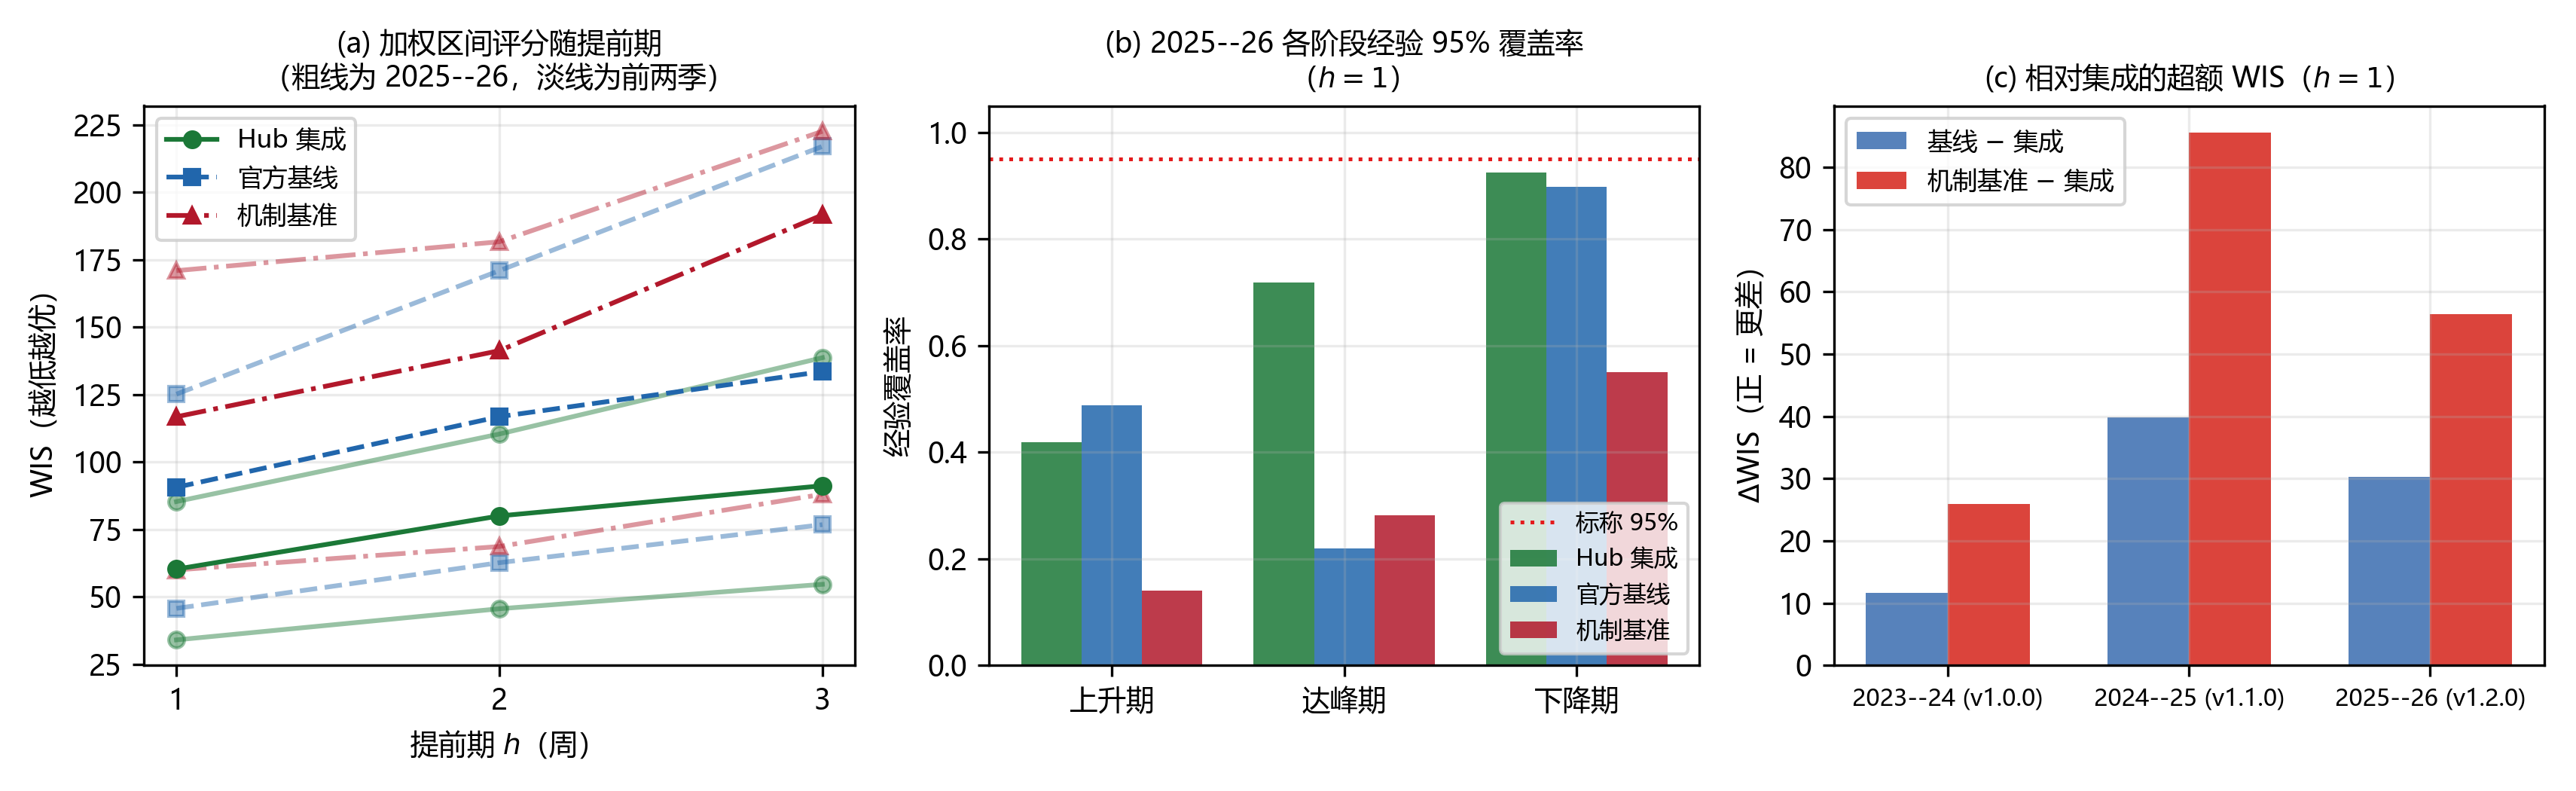
\includegraphics[width=\textwidth]{reports_v3/figures/fig_flusight_audit.png}
\caption{\textbf{CDC FluSight 三个连续赛季外部审计与峰值相对位置分层校准特征。}(a) 三个锁定赛季加权区间评分（WIS）随提前期 $h$ 的衰减轨迹（实线粗体为 2025--26 赛季并附 95\% Bootstrap CI 阴影带，虚线与点线为前两季对照），展示 Hub 集成对官方基线与启发式插件式机制预测器的持续优势；(b) 各阶段经验 95\% 预测区间覆盖率（$h=1$，柱状为 2025--26 赛季，散点为前两季对照，橙色虚线为标称 95\% 水平），在多个模型—赛季组合中观察到疫情峰前期经验覆盖率较低（在 2025--26 赛季三模型覆盖率为 0.140--0.488，全三赛季跨度为 0.140--0.852，见表~\ref{tab:phase_stratification}）；(c) $h=1$ 时各模型相对集成的超额 WIS 及配对 95\% Bootstrap 置信区间（三个赛季中，相对集成的配对 WIS 差置信区间均未跨越 0）。}
\label{fig:flusight_audit}
\end{figure}

本项分层审计给出三项经验观察（均为 $h=1$ 的严格配对评估结果）：
\begin{itemize}[leftmargin=*,itemsep=0.2pt,topsep=1pt,parsep=0pt]
\item \textbf{峰后期的近标称校准}：在疫情峰后期，Hub 集成模型的 95\% 预测区间经验覆盖率为 \textbf{0.925--0.964}，接近标称水平；官方基线为 0.881--0.922，而启发式机制预测器覆盖率为 0.381--0.575。
\item \textbf{峰前期的经验覆盖率偏低}：进入峰前期后，Hub 集成模型的 95\% 覆盖率在三个赛季分别为 \textbf{0.852}、\textbf{0.589} 和 \textbf{0.419}，官方基线分别为 0.759、0.539 和 0.488，启发式机制预测器分别为 0.370、0.385 和 0.140。除 2024--25 赛季启发式机制预测器（0.385 对 0.381）外，多数模型—赛季组合的峰前期覆盖率系统性低于其峰后期水平。需注意，2025--26 赛季峰前期评估单元较少（$n=43$），其覆盖率点估计具有较宽的 Wilson 95\% 置信区间（Hub 集成 $[0.284, 0.567]$，基线 $[0.346, 0.632]$，机制预测器 $[0.066, 0.273]$），应结合样本量谨慎评估。
\item \textbf{阶段样本分布与数据回填特征}：严格四方交集下峰前期评估单元在各赛季为 43--343，峰值窗口为 32--132，峰后期为 840--1,301，反映了流行季自然发展中峰后持续周数较长的宏观特征。同时，终报真值在峰前期往往包含显著的向上回填修订，导致即使基于初报信息作出了良好预测，在事后终报核验时也会产生结构性的惩罚放大。
\end{itemize}

基于全局峰值相对位置的事后分层表明，在多个模型—赛季组合中，峰前期经验覆盖率低于峰后期。需说明，参数外推相对方差项 $P_{\text{exact}}(h; s) = \exp(2h^2s^2) - 2\exp(\tfrac{1}{2}h^2s^2) + 1$ 显式依赖步长 $h$ 与对数斜率标准误 $s$，并不直接包含增长率水平 $R$；因此，峰前期覆盖率的下降不能简单在代数上单因果归结为增长乘子 $R$ 的指数放大。峰前期覆盖率偏低可能与非平稳动力学、突发变点、公众自发防护、数据回填等多重现实因素综合相关。在公共卫生运筹实践中，峰前期的欠覆盖特征提示业务预测系统的标称预测区间需结合安全裕度进行审慎解读，避免将未校准的窄区间直接作为资源调度的刚性决策上限。

\subsection{COVIDhub-ensemble 多波次历史对照}\label{sec:covidhub_control}

为检验上述外部审计规律在跨病原、大流行情境下的描述性可迁移性，本节保留对美国 COVID-19 预测枢纽官方集成（COVIDhub-ensemble）在早期 Delta 与 Omicron 两大典型暴发波次中连续 12 个逐周预测原点的历史对照（图~\ref{fig:hub_skill} 与补充材料附表 S9）。

\begin{figure}[htbp]
\centering
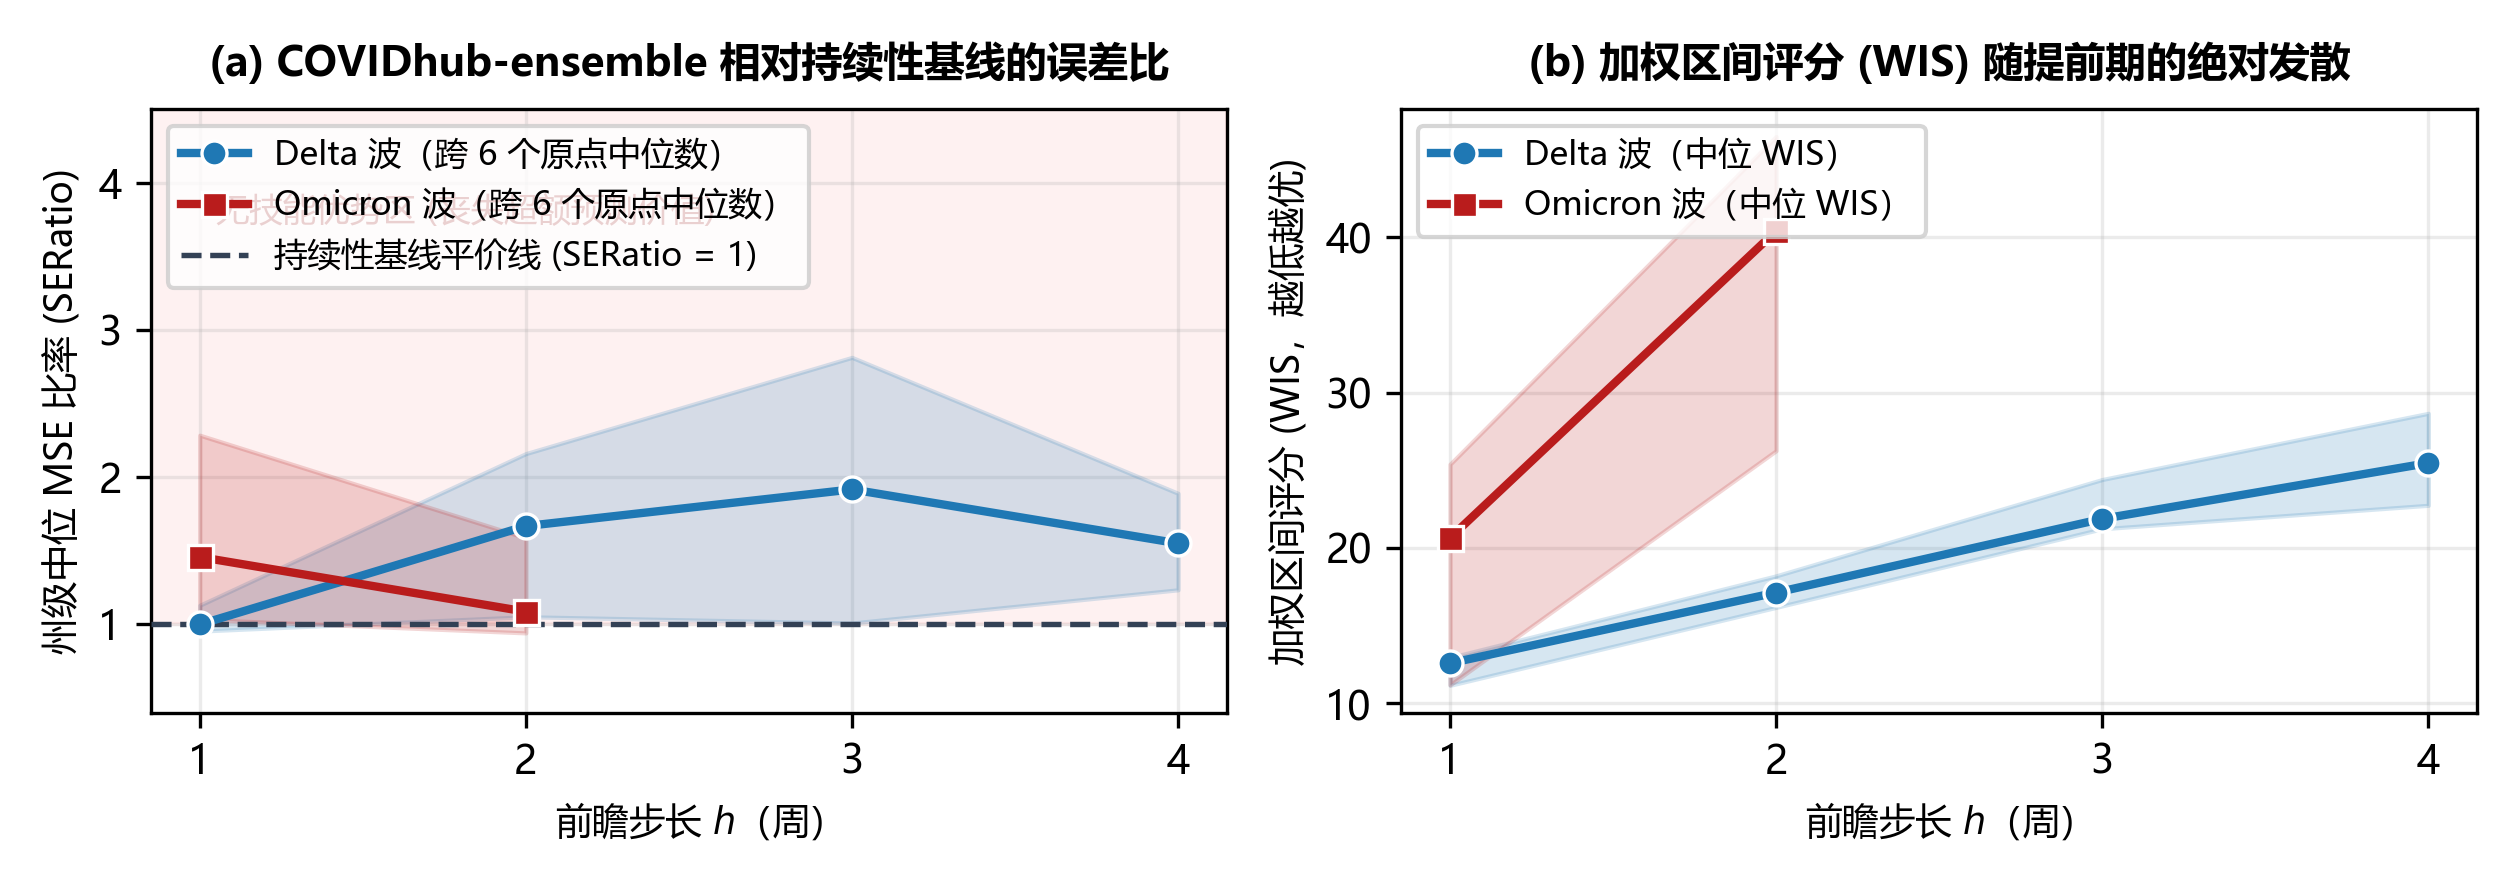
\includegraphics[width=\textwidth]{reports_v3/figures/fig_hub_skill.png}
\caption{\textbf{COVIDhub-ensemble 州级相对技能变化与原始尺度 WIS 上升。}(a) 跨州中位平方误差比率 $\text{SERatio}$（相对持续性基线）随前瞻周数的变化，灰色阴影带为跨原点四分位距（IQR），黑色虚线为与持续性基线平价（$\text{SERatio} = 1$）。Delta 与 Omicron 两波共 12 个预测原点中有 11 个在 1--2 周内达到或穿透平价线（唯一例外为 Delta 2021-08-02 原点，其跨州中位 SERatio 在四个前瞻步长上均低于 1，最大仅 0.939），丧失相对技能优势（注：Omicron 波次受官方预测枢纽历史归档中部分长步长预测未标准化及数据缺失限制，评估步长有效覆盖至 $h=2$）；(b) 原始计数尺度下的加权区间评分（WIS）随提前期上升，表明概率预测综合误差随步长恶化；由于 WIS 同时受到目标规模、位置偏差和区间离散度影响，该结果不能单独解释为预测方差或不确定性的纯粹膨胀。}
\label{fig:hub_skill}
\end{figure}

\subsection{模型参照误差差额与候选失配来源}\label{sec:gap_attribution}

综合第 5 节的州级面板分析与本节的外部审计，需在数学上严格区分两类量纲不同的模型参照误差差额：

\noindent\textbf{第一类：模型参照下的平方误差差额（$\mathrm{Gap}^{\text{SE}}_h$）。}在点预测与平方损失维度下，以宏观机制工作模型推导的过程方差 $V^{\text{model}}_h = \text{CV}^2_{\text{macro}}(h)\,(I_0 R^h)^2$ 为参照：
\begin{equation}
\mathrm{Gap}^{\text{SE}}_h \equiv \widehat{\text{MSE}}_{\text{obs}}(h) - V^{\text{model}}_h.
\label{eq:gap_se}
\end{equation}
两类差额具有明确的分析边界：(i) $V^{\text{model}}_h$ 仅为固定宏观更新模型与固定插件参数下的模型内方差基准；(ii) $\mathrm{Gap}^{\text{SE}}_h$ 是经验均方误差与模型方差之间的代数差额，在有限样本或模型设定偏误下并不保证非负，亦不等于定理~\ref{thm:sharp_floor} 中处处非负的理论超额风险 $(m_h - \delta_h)^2$。第 5.4 节的相对误差记账可视为该绝对平方误差差额在特定归一化口径下的对应形式。

\noindent\textbf{第二类：配对概率评分差（$\Delta\text{WIS}$）。}外部审计的核心评价指标为基于 23 分位数的加权区间评分（WIS\citep{bracher2021evaluating}）。WIS 是针对所报告中位数与中心预测区间的严格适当评分规则（Proper Scoring Rule）。对于两个预测体系 $A$ 与 $B$（如 $A = \text{官方基线或启发式插件式机制预测器}$，$B = \text{Hub 集成}$），定义样本配对概率评分差 $\Delta\mathrm{WIS}_{A, B}(h) \equiv \overline{\mathrm{WIS}}_A(h) - \overline{\mathrm{WIS}}_B(h)$。需要明确：$\Delta\mathrm{WIS}$ 属于概率预测分布间的配对评分差，综合反映了预测分布的位置偏差、离散充盈度与尾部惩罚，不等同于平方损失下的不可约条件方差地板。

上述两类差额的主要候选失配机制涵盖：(1)~\textbf{均值模型误设与非平稳漂移}：真实再生数随人群自发防护、政策介入而动态时变，静态指数增长假设在多周外推中必然偏离；(2)~\textbf{监测系统的测量与修订扰动}：医院报告延迟导致预测原点处所见并非真实发病全貌，事后向上的回填修订直接拉大了前瞻偏差；(3)~\textbf{预测不确定性的结构性低估}：现有预测系统在部分峰前期未能充分反映结构变点和分布外波动，表现为预测区间系统性偏窄；该特征见 图~\ref{fig:flusight_audit}(b)。上述误差分解表明：NB2 机制视界作为“现实预警时效的经验参考外包络”与现有实测证据保持一致，现实业务系统要逐步逼近该基准，其攻关重点应聚焦于提升疫情峰前期的数据感知度与动态不确定性校准算法。

\noindent\textbf{州际空间相关性。}51 个州级辖区受共同季节与毒株驱动存在空间相关；10 个 HHS 区域整群聚类自助检验表明全部九个赛季--步长组合的配对差区间仍严格不跨零（第~\ref{sec:flusight_protocol} 节），证实了集成模型相对基线的稳定优势。

\section{讨论与公共卫生启示}\label{sec:discussion}

\subsection{公共卫生决策分级场景与可预测视界映射}

公共卫生决策对前瞻窗口与误差容忍度有分级需求。为考察容错阈值对机制视界的影响，补充材料附表 S7 测算了四档典型容忍度（$\tau \in \{0.20, 0.35, 0.50, 0.70\}$）下的 NB2 模型内机制视界演化（该阈值仅为示意性映射，未由具体公卫损失函数校准）。结果显示：面临重症 ICU 扩容等高成本刚性决策时（$\tau = 0.20$），州级中位 NB2 模型内机制视界收缩至 0.4--1.5 周（Omicron 为 0.8 周），在该示意性容忍度设定下，提示不宜将中远期点预测单独作为刚性决策依据；常态物资调配（$\tau = 0.35$）与社会面准备（$\tau = 0.50$）阶段拓展至 1.2--4.1 周；放宽至 $\tau = 0.70$ 时拓宽至 3.9--11.0 周。国家级聚合视界通常高于州级中位数（表~\ref{tab:horizons}），直接采用国家级聚合值可能高估部分州级辖区的可操作预警窗口。实测业务时效约为机制视界的 $1/4\sim 1/1.1$，应急调度需预留充足安全余量。

\subsection{从理论机制视界到预警响应的运筹转化与公平性考量}\label{sec:operational_translation}

从数理极限向应急运筹转化需建立非对称风控边界\citep{parag2025asymmetric}。诊断性视界 $h^*$ 刻画统计可信跨度，有效预警提前量受制于暴发确认延迟：$\Delta t_{\text{alert}} = h^* - t_{\text{detect}}$（$t_{\text{detect}}$ 为跨越定理~\ref{thm:fisher} 样本量基准所需耗时）。若早期监测网络稀疏导致确认过迟，干预窗口将被挤压；决策者应在 $h \le h^*$ 内结合分级容错动态设定触发阈值。

健康公平性层面，定理~\ref{thm:fisher} 表明参数辨识精度正比于有效样本量 $C$。在两地区其他动力学参数、初始规模和过程方差近似相同，且视界主要受参数辨识误差约束的领先阶条件下，若有效样本量与报告率成正比（欠发达社区有效报告率 $\rho_{\text{low}} \ll \rho_0$），参数推断方差按 $\rho_0/\rho_{\text{low}}$ 放大，理论机制视界在参数方差主导体制下近似满足相对标度关系：$\frac{h^*_{\text{low}}}{h^*_0} \approx \sqrt{\frac{\rho_{\text{low}}}{\rho_0}}$。需强调，该平方根标度仅在过程方差可忽略（$\text{CV}^2_{\text{macro}} \ll \tau^2$）的理想参数敏感区成立；在本文实测的州级工作点中，宏观过程方差占比普遍高达 $73\%\sim 89\%$（图~\ref{fig:state_horizons}b），报告率减半往往直接使得观测发病规模 $I_0$ 减半，导致过程变异系数翻倍并可能直接击穿容忍阈值，致使实际预警视界完全消失。因此，$\sqrt{\rho}$ 关系代表了监测削弱时预警损失的乐观上限，提示资源配置部门必须向薄弱地区倾斜常态化监测网络以防范预警盲区。

\subsection{研究局限性与未来拓展方向}\label{sec:limitations}

{\fontsize{8.0pt}{10.2pt}\selectfont
\noindent\textbf{（一）实证与方法学适用边界}

\begin{enumerate}[leftmargin=*,itemsep=0pt,topsep=1pt,parsep=0pt]
\item \textbf{代数差额反映真实业务扰动}：在 21 个阶段--步长配置中，模型—观测代数差额跨州中位占比为 $55.0\%$（$h=1$ 为 $45.4\%$），表明机制方差与参数外推构成了预测误差的刚性基底，而其余差额由行为自适应、报告回填及模型结构性偏离所共同吸收；时变漂移作为有界敏感性分析处理。
\item \textbf{业务时效对基线与数据流状态的敏感性}：相对持续性基线的州级时效为 1.0--4.3 周，相对局部线性基线在约 1 周追平；回测基于终报数据，反映数据充分沉淀后的理论能力上限，面临初报延迟时有效时效预期更短。
\item \textbf{跨病原覆盖范围}：COVIDhub 对照覆盖早期 Delta 与 Omicron 两波约 6 个月，目前尚缺乏 RSV 官方预测枢纽的长期公开历史归档。
\item \textbf{微观与宏观离散度的层级边界}：主口径采用宏观更新模型与有效离散度 $k_{\text{agg}}$，微观分支闭式在宏观尺度仅作参数敏感性参照，二者不可跨层级直接混用。
\item \textbf{宏观方差结构是首要的不确定性来源}：全部州级视界均在固定离散度 NB2 更新模型下求得，其相对过程方差含几何项 $(1+1/k_{\text{agg}})^h$。在同一面板与同一参数集上改用线性过度离散的 NB1／准 Poisson 或 Poisson 结构后，各阶段中位视界由 2.20--7.12 周延长至 2.93--9.34 周（1.06--1.53 倍）与 5.07--11.10 周（1.56--2.56 倍，均值 1.96 倍）（表~\ref{tab:alt_variance}），即几何发散项贡献了本文视界的约一半。该结构性差异的量级超过推断窗口（$\pm 45\%$）与 $k_{\text{agg}}$ 截断（$\le 7.4\%$），且长于准入门槛所引致的向上偏置，故读者应以"固定 NB2 工作模型条件下的基准"而非"数据自身的视界"来理解本文的主数值。
\item \textbf{推断窗口的结构权衡}：5--10 周窗口选择带来 $-48.7\%$ 至 $+44.6\%$ 的中位视界浮动（补充材料附表 S6），体现了压缩估计标准误与引入非平稳漂移之间的统计权衡。
\item \textbf{阶段划分的事后全局属性}：基于全局峰值相对位置划分阶段，峰前期覆盖率偏低反映了流行上升期高动态扰动下的系统性特征，不宜归结为局部单因果效应。
\item \textbf{宏观方差结构的比较拓展}：本文以固定离散度 NB2 作为基准工作模型，未来宜系统拓展至动态离散度、状态空间及泊松混合过程的样本外综合对比。
\item \textbf{模型族谱与推断检验的拓展}：微观分析聚焦于标准负二项与泊松对比，未来可进一步拓展至零膨胀负二项及混合治愈模型。
\item \textbf{空间相关性的多层级建模}：10 个 HHS 大区整群聚类自助检验表明配对差显著不跨零，后续可结合空间计量自回归模型深入解析跨州协同动态。
\item \textbf{适用域截断的物理约束}：对极端发病外推超出单季自然跨度（$\ge 20$ 周）的测算值实施了截断，提示在超长前瞻期需引入流行动力学易感耗竭非线性机制。
\item \textbf{队列监测完整性与地域边界}：实证基于美国 51 个辖区三种呼吸道病原及两个海外队列。其中香港接触追踪网络依托密集城市流调，漏检率较低；几内亚埃博拉队列受制于乡村资源与社区阻力，可能存在隐匿传播链，导致离散度估计受不同程度的选择性报告偏差影响。
\end{enumerate}

\noindent\textbf{（二）理论拓展方向}

本文聚焦早期分支增长，未耦合易感耗竭非线性负反馈（SIR 类）并隐含均匀混合。将视界理论与非线性 Hamilton--Jacobi 波动方程或元种群分支网络结合推导跨峰全相位闭式解是重要深化方向\citep{parag2026threshold}。此外，初值 $I_0$ 的在线估计不确定性目前被代数差额吸收，其因果剥离与多源异构信号（污水监测、搜索指数、基因组丰度）融合增益边界均属关键前沿。\par}

\vspace{-2pt}
\section{结论}\label{sec:conclusion}

本文系统构建了区分理论条件风险地板、NB2 模型内过程方差、插件预测风险与现实业务误差的分层分析框架。理论层面，本文确立了平方损失下条件均值预测器的锐条件方差地板，刻画了个体负二项生成机制下的 Fisher 信息下界（实测离散度下对应有效样本量门槛 $C \ge 2{,}162\text{--}6{,}593$），并推导了宏观 NB2 递归更新模型在有限步长下的精确方差闭式与参数不确定性指数放大律。实证层面，依托四层证据架构的系统检验表明：(1) 微观接触追踪数据高度支持负二项过度离散假说（$\Delta\text{AIC}$ 达 93.9--244.0，Bootstrap 方差与 Cramér--Rao 下界比值为 0.98--1.06）；(2) 在覆盖美国最多 51 个州级辖区、七个重大流行波次的住院面板中，5 周基准窗口下测得的插件式 NB2 机制视界跨州中位数为 2.2--7.1 周，多窗口极值包络覆盖 1.52--8.07 周，系统性高于实测绝对误差视界（1.2--3.9 周）：阶段级中位数之比为 1.11--4.00 倍，在同一辖区上严格配对的 294 个逐州单元的中位比率为 1.79（IQR [1.10, 3.36]），其中 78.9\% 构成外包络，但该外包络\textbf{并非逐点成立}，在低计数阶段约三分之一单元反号；(3) 误差记账表明在 21 个阶段—步长配置中有 20 个配置的模型—观测代数差额跨州中位数为正（中位占比达 55.0\%），但机制分量与实测误差的关系存在阶段异质性：在低发病短步长配置（如 JN.1 $h=1$）中模型方差可达实测误差的 114.1\%，表明机制基准刻画的是无外生扰动理想状态的统计参考外包络而非逐点刚性下界；(4) CDC FluSight 三个连续赛季的外部版本化审计证实，启发式机制基准预测器在无报告延迟的终报条件下仍表现出显著的经验欠覆盖（标称 95\% 区间实测覆盖率仅 0.405--0.554），且在疫情峰前期校准偏离尤为突出。上述理论与实证结果共同表明，基于内在生成机制推导的机制视界，可作为现实业务时效在统计学意义上的经验参考外包络。这一结论为公共卫生预警系统的应急资源调度设定了客观的统计可信窗口，也为未来发展融合多源监测信号、具备动态不确定性感知能力的下一代流行病预测系统提供了严谨的基准参照。

\clearpage
\appendix
\section*{附录：核心定理数理证明要点与详尽推导索引}
\addcontentsline{toc}{section}{附录：核心定理数理证明要点与详尽推导索引}

针对全文 17 项核心数理结论（定理 1--5、引理 1--4、命题 1--4、推论 1--4），本文建立了一套双层推导记录体系：正文呈现结论与机理直觉，本附录给出核心代数证明要点与全景推导索引表（表~\ref{tab:derivation_roadmap}）；逐行展开的详尽代数运算（包括完整矩阵分块求逆、微分方程积分测度分类与多项式因式分解步骤）系统收录于随稿提交的独立推导手册《过度离散传染病更新模型的条件预测风险与视界》（\textit{Conditional Risk, Exact Macro Variance, and Forecast Horizons}，以下称"推导手册"）。该手册按方法而非按结论组织，故表~\ref{tab:derivation_roadmap} 末列给出每项结论对应的手册节名：其中 15 项可直接溯源至手册相应节，推论~\ref{cor:near_crit_horizon} 与推论~\ref{cor:establishment} 的逐步推导未单列于手册，仅由本附录"核心定理数理证明要点"给出证明梗概，此处如实标注。

\begin{table}[htbp]
\centering
\fontsize{7.0pt}{8.4pt}\selectfont
\setlength{\tabcolsep}{2.0pt}
\caption{全文核心定理、引理与推论的数理推导全景索引目录（末列「推导出处」已逐条对齐随稿提交的推导手册实体节名）}\label{tab:derivation_roadmap}
\begin{tabular}{@{}>{\raggedright\arraybackslash}p{2.3cm}>{\raggedright\arraybackslash}p{2.6cm}>{\raggedright\arraybackslash}p{1.6cm}>{\raggedright\arraybackslash}p{4.6cm}>{\raggedright\arraybackslash}p{3.4cm}@{}}
\toprule
结论编号与名称 & 核心物理 / 统计内涵 & 正文位置 & 核心数理工具与关键证明步骤 & 推导出处 \\
\midrule
定理~\ref{thm:sharp_floor} 锐条件方差地板 & 平方损失下不可约误差极限 & 式~\eqref{eq:sharp_floor_identity} & $L^2(\Omega,\mathcal{F}_t,\mathbb{P})$ 条件期望正交投影，交叉项几乎处处为零 & 手册 §3 条件风险恒等式（精确条件平方风险恒等式） \\
\addlinespace[3pt]
引理~\ref{lem:branch_moments} 分支过程两阶段矩 & 微观发病均值与方差递推 & 式~\eqref{eq:lem1_var} & 全期望与全方差分解，一阶非齐次差分方程 $R^{2n}$ 伸缩求和 & 手册 §2.2 个体层 Galton--Watson 参考模型（个体层全代方差） \\
\addlinespace[3pt]
引理~\ref{lem:cv_floor} 变异系数与方差地板 & 群体内在相对方差饱和极限 & 式~\eqref{eq:cv_floor} & 相对方差因式分解，超临界 $R^{-h}\to0$ 与近临界连续延拓 & 手册 §2.2（同上） \\
\addlinespace[3pt]
引理~\ref{lem:param_amplification} 参数对数正态放大 & 估计量非线性外推误差 & 式~\eqref{eq:param_amplification} & 对数正态对偶阶矩母函数展开，Jensen 凸性多项式期望展开 & 手册 §4.1 共享对数正态参数下的后验预测矩 \\
\addlinespace[3pt]
定理~\ref{thm:horizon} 视界可加分解与求根 & 双源误差正交分解与机制视界 & 式~\eqref{eq:relmse_decomp} & 条件期望正交性保证无交叉项，全方程严格单调性保证唯一数值根 & 手册 §4 后验全方差分解；§3 阈值视界的定义 \\
\addlinespace[3pt]
推论~\ref{cor:near_crit_horizon} 近临界视界解析解 & 阈值相变点预测视界收缩 & 式~\eqref{eq:crit_horizon} & 临界线性方差累积展开，一元二次代数方程正实根解析解 & 本附录证明要点（手册未单列该推论的逐步推导） \\
\addlinespace[3pt]
定理~\ref{thm:monotonicity} 相对均方误差单调性 & 预测误差随前瞻步长严格递增 & 定理~\ref{thm:monotonicity} & 构造辅助函数 $g(y)$，在区间 $y>1$ 与 $0<y<1$ 证明因式同号恒正 & 手册 §2.3 宏观层固定离散度更新（方差增量正值性） \\
\addlinespace[3pt]
命题~\ref{prop:qsd} 反射扩散与特征标度 & 临界慢化涨落动力学直觉 & 式~\eqref{eq:qsd_density} & 零概率流调和方程积分求平稳密度，动力学重标度消去 $N$ & 手册 §7.1 带下截断的反射扩散辅助密度 \\
\addlinespace[3pt]
推论~\ref{cor:establishment} 单种子建群概率 & 强超扩散对持续定殖的抑制 & 式~\eqref{eq:pgf_fixed_point} & 负二项概率母函数不动点 $q=G(q)$ 二阶泰勒展开提取 $(1-q)$ & 本附录证明要点（该推论的逐步推导未收录于手册） \\
\addlinespace[3pt]
定理~\ref{thm:fisher} Fisher 信息与 CRB 界 & 早期参数辨识数据充分性下限 & 式~\eqref{eq:cramer_cn} & 得分函数二阶导负期望，交叉偏导期望为零确立参数渐近正交 & 手册 §6.1 条件负二项似然 \\
\addlinespace[3pt]
推论~\ref{cor:crb_horizon} 样本量约束机制视界标度 & 监测样本量对视界的外在约束 & 式~\eqref{eq:crb_horizon} & CRB 理论方差代入连续视界方程反解乐观前瞻代际标度 & 手册 §6.2 单位暴露的理想基准 \\
\addlinespace[3pt]
命题~\ref{thm:t5} 宏观方差线性累积律 & 固定聚合离散度更新噪声累加 & 命题~\ref{thm:t5} & 截断对数差分 $\Delta L_t$ 规避 $Z_{t-1}=0$ 奇异性，大均值与大 $k_{\text{agg}}$ 展开（大均值界含 $\psi_1$） & 手册 §2.4 正计数值截断对数协议与三伽马极限（大均值下的三伽马极限与矩收敛） \\
\addlinespace[3pt]
命题~\ref{prop:t5r} 环境噪声持续性漂移 & 增长率时间自相关方差累积 & 命题~\ref{prop:t5r} & 平稳自协方差级数求和；单位根下自然数平方和通项超线性发散 $\sim h^3/3$ & 手册 §5.1--§5.2 AR(1) 增长率的条件累积方差 \\
\addlinespace[3pt]
推论~\ref{cor:pop_floor} 宏观抽样 $h/k_{\text{agg}}$ 律 & 跨代独立增量大样本噪声地板 & 式~\eqref{eq:pop_floor} & 截断对数 Delta 展开，大均值与大 $k_{\text{agg}}$ 下为 $1/k_{\text{agg}}$（大均值界为 $\psi_1$） & 手册 §2.4（同命题 2） \\
\addlinespace[3pt]
定理~\ref{thm:macro_exact} 宏观有限步精确方差 & 固定 $k_{\text{agg}}$ 更新模型精确方差 & 式~\eqref{eq:macro_var_closed} & 一阶非齐次差分方程伸缩求和（递推式见式~\eqref{eq:macro_var_recurrence}） & 手册 §2.3 固定 $k$ 宏观模型的精确有限步方差 \\
\addlinespace[3pt]
引理~\ref{lem:macro_boundaries} 稳定边界极限 & 浮点运算消除相消误差 & 式~\eqref{eq:bound_q_eq_R} & 洛必达法则求差商极限；$R=1$ 展开；$k\to\infty$ 泊松极限；$I_0\to\infty$ 宏观地板 & 手册 §2.3（同定理 5，含可去奇点与边界极限） \\
\addlinespace[3pt]
命题~\ref{prop:posterior_mixture} 对数正态后验混合 & 完全贝叶斯预测方差与超额风险 & 式~\eqref{eq:mixture_full_var} & 全方差公式，对数正态对偶阶矩有限和展开，Jensen 不等式超额风险 & 手册 §4.1（同引理 3） \\
\bottomrule
\end{tabular}%
\end{table}




\clearpage
{\fontsize{8.5pt}{10.8pt}\selectfont
\subsection*{核心定理数理证明要点}

\begin{enumerate}[itemsep=0.2pt,topsep=0.5pt,parsep=0pt]
\item \textbf{定理~\ref{thm:sharp_floor}}：正交拆分 $Y_{t+h}-\delta_h = (Y_{t+h}-m_h)+(m_h-\delta_h)$，交叉项 $(m_h-\delta_h)\mathbb{E}[Y_{t+h}-m_h\mid\mathcal{F}_t]=0$，得 $\mathcal{R}_h = V_h+(m_h-\delta_h)^2\ge V_h$，等号当且仅当 $\delta_h=m_h$。
\item \textbf{引理 1--2}：全方差公式得差分方程 $V_n-R^2V_{n-1}=\sigma^2I_0R^{n-1}$，$R^{2n}$ 伸缩求和导出 $\text{CV}^2(h)=(1+R/k)(1-R^{-h})/[I_0(R-1)]$，超临界下饱和于 $\text{CV}^2_\infty$。
\item \textbf{引理 3 与定理~\ref{thm:horizon}}：对数正态矩母 $\mathbb{E}[Y^m]=\exp(m^2s^2/2)$ 展开 $P_{\text{exact}}(h)=\exp(2h^2s^2)-2\exp(h^2s^2/2)+1$；假定 (A4) 正交性确立 $\text{RelMSE}=\text{CV}^2+P_{\text{exact}}$，单调性保证 $h^*$ 唯一。
\item \textbf{定理~\ref{thm:monotonicity}}：$\text{CV}^2$ 增量 $(1+R/k)/(I_0R^{h+1})>0$；辅助函数 $g(y)=(y^{h_2}-y^{h_1})(y^{h_2}+y^{h_1}-2)$ 在 $y>1$ 与 $0<y<1$ 均同号恒正。
\item \textbf{定理~\ref{thm:fisher}}：NB 对数似然二阶导负期望得 $I_1(R)=k/[R(R+k)]$；交叉偏导期望为零确立渐近正交；Wald 型检验反解样本量门槛。
\item \textbf{定理~\ref{thm:macro_exact}}：全方差法则得 $V_{t+1}=qV_t+I_0R^{t+1}+I_0^2R^{2t+2}/k_{\text{agg}}$（$q=R^2c$），除以 $q^{t+1}$ 裂项求和，利用 $q-R^2=R^2/k_{\text{agg}}$ 合并得 $V_h=I_0R(q^h-R^h)/(q-R)+I_0^2(q^h-R^{2h})$。
\item \textbf{命题~\ref{thm:t5} 与推论~\ref{cor:pop_floor}}：截断对数差分 $\Delta L_t \equiv L_t - L_{t-1}$ 与 $b_t^\Delta$ 规避 $Z_{t-1}=0$ 奇异性，确立鞅差创新有限性；在固定有限提前期、各步均值充分大及高阶矩一致可积性下，$(Z_t\vee 1)/\mu_t \xrightarrow{d} G_t$ 确立一、二阶矩收敛至 $\psi(k)-\ln k$ 与 $\psi_1(k)$；大 $k_{\text{agg}}$ 级数展开截断给出 $1/k_{\text{agg}}$ 一阶累积近似。
\end{enumerate}

\subsection*{附录支持说明与补充材料索引}

为保持正文叙事紧凑聚焦，更详尽的数理推导、完整证明步骤、参数敏感性网格及辅助诊断图表收录于随稿提交的两份补充材料：推导手册《过度离散传染病更新模型的条件预测风险与视界》（\path{derivations/derivations_manual.pdf}）与《补充材料：支持表格 S1--S9》（\path{supplementary/supplementary_tables.pdf}）。主要内容包括：
\begin{enumerate}[itemsep=0.2pt,topsep=0.5pt,parsep=0pt]
\item \textbf{数理证明手册（推导手册 §1--§7）}：收录全文 17 项数理结论中 15 项的逐行代数演算、分块矩阵求逆细节、边界微分方程积分展开与数值相消控制证明（另 2 项见本附录证明要点，见表~\ref{tab:derivation_roadmap} 末列标注）。
\item \textbf{符号、样本量与数据溯源（表 S1--S3）}：主要符号与口径对照表（表 S1）、定理~4 验证的完整参数网格与理想样本量基准（表 S2，50{,}000 次蒙特卡洛）、各分析对象的数据源与潜在泄漏核查表（表 S3）。
\item \textbf{州级面板口径与敏感性（表 S4--S7）}：四类视界口径定义与层级归属（表 S4）、七阶段六口径视界全景对照（表 S5）、推断窗口与 $k_{\text{agg}}$ 截断敏感性矩阵（表 S6）、不同容错门槛下的多层级预警映射（表 S7）。
\item \textbf{预测枢纽审计明细（表 S8--S9）}：CDC FluSight 三赛季分步长完整评分面板（表 S8，逐单元与逐辖区明细另见随包 CSV）、COVIDhub-ensemble 12 预测原点逐周技能衰减明细（表 S9）。
\end{enumerate}

\noindent{\textbf{数据与代码可得性声明。}} 本文全部输入数据与分析代码作为附件随稿提交，共 237 个文件（约 203 MB），涵盖州级周度住院面板（4 个）、个体传播链队列（7 个）、COVIDhub 历史对照原点（13 个）及 CDC FluSight 三个锁定赛季的原始预测输入文件（204 个：v1.0.0 62 个、v1.1.0 85 个、v1.2.0 57 个）。上述每个文件均已逐文件固化 SHA-256 校验和，清单见 \texttt{data/input\_hashes.json}；本包的一致性验收门禁 \texttt{scripts\_v2/check\_consistency.py} 会对该清单逐条复核，确保全部评分表与附图逐字节可复现。数据来源均为公开监测与公开预测枢纽档案：州级住院面板取自美国 CDC 数据门户终报冻结快照（经 HHS Protect 与 NHSN 沉淀发布）；传播链取自 Adam 等\citep{adam2020clustering} 与 Faye 等\citep{faye2015chains} 公开发表的接触追踪队列；预测档案取自 CDC FluSight 与 COVID-19 Forecast Hub 的公开版本化提交。为满足双盲评审要求，含长期 DOI 的完整资产包公开归档将于论文录用后发布；评审期间可经编辑向作者索取。

\vspace{0.2em}
\noindent{\textbf{利益冲突声明。}} 作者声明不存在利益冲突；双盲评审期间作者贡献与致谢暂略。\par}

\clearpage
\noindent{\heiti\zihao{4}\bfseries 参考文献：}\vspace{0.1em}
\begin{multicols}{2}
{\fontsize{7.5pt}{9.0pt}\selectfont
\setlength{\bibsep}{1.0pt}
\renewcommand{\refname}{}
\vspace*{-2.0em}
\bibliographystyle{unsrtnat}
\bibliography{references}
}
\end{multicols}

\end{document}
